\documentclass[a4paper,openany,oneside,fontset=none]{ctexbook}
% \usepackage[fontset=none]{ctex}

\ctexset{
	chapter={
        name = {第,章}
    },
}
\usepackage{amsthm}
\usepackage{amsmath}
\usepackage{amssymb}
\usepackage{graphicx}
\usepackage{geometry}
\usepackage{booktabs}
\usepackage{makecell}
\usepackage{multirow}
\usepackage{float}
\usepackage{enumerate}
\usepackage{fancyhdr}
\setlength{\headheight}{12.7pt}
\pagestyle{fancy}
\fancyhead[L]{By Ling Yu}
\geometry{left=2.5cm,right=2.5cm,top=2.5cm,bottom=2.5cm}

\labelformat{equation}{公式 (#1)}  % 加括号
\usepackage[bookmarksopen=true,unicode,psdextra]{hyperref}
\usepackage{bookmark}
\hypersetup{
    hidelinks,
	colorlinks=true,
	allcolors=black,
	pdfstartview=Fit,
	breaklinks=true,
    % bookmarks=true,     % 显示书签
    bookmarksopen=true, % 初始展开所有书签
    bookmarksnumbered=true, % 给书签添加章节编号
}
% \usepackage{bookmark}
\title{\textbf{概率论与数理统计}}
\author{Ling Yu}
\date{\today}


\newtheorem{example}{\indent 例}[section]            % 整体编号
\newtheorem{algorithm}{\indent 算法}
\newtheorem{theorem}{\indent 定理}[section]  % 按 section 编号
\newtheorem{definition}{\indent 定义}[section]
\newtheorem{axiom}{\indent 公理}
\newtheorem{property}{\indent 性质}[section]
\newtheorem{proposition}{\indent 命题}
\newtheorem{lemma}{\indent 引理}
\newtheorem{corollary}{\indent 推论}[section]
\newtheorem{remark}{\indent 注解}
\newtheorem{condition}{\indent 条件}
\newtheorem{conclusion}{\indent 结论}
\newtheorem{assumption}{\indent 假设}
\numberwithin{equation}{section}
\newenvironment{solution}{\begin{proof}[解]}{\end{proof}}


\setCJKmainfont[BoldFont = PingFangSC-Semibold, ItalicFont=PingFangSC-Regular]{PingFangSC-Medium}
\setCJKsansfont{FZHei-B01}[BoldFont={Source Han Sans SC Medium}]
\setCJKmonofont{FZFangSong-Z02}
\newCJKfontfamily\songti{FZShuSong-Z01S}[BoldFont={Source Han Serif SC}]
\newCJKfontfamily\heiti{FZHei-B01S}[BoldFont={Source Han Sans SC Medium}]

\begin{document}
% \begin{sloppypar}
\maketitle
% \pdfbookmark[0]{目录}{toc}
% 将目录页添加到书签
% \pdfbookmark{\contentsname}{目录}
\newpage
\phantomsection
\addcontentsline{toc}{chapter}{\contentsname}
\tableofcontents
% \addcontentsline{toc}{section}{目录}

\newpage
\setcounter{page}{1}
% \clearpage % 新建一页,开始正文内容

\chapter{随机事件与概率}
\section{随机事件间的关系及运算}
\subsection{事件间的运算规律}
\begin{enumerate}
    \item 交换律 $A \cup B = B \cup A,AB = BA$
    \item 结合律 $(A \cup B) \cup C = A \cup (B \cup C)$ $(AB)C = A(BC)$
    \item 分配律 $(A \cup B) \cap C = (A \cap C) \cup (B \cap C) = AC \cup BC$
          $(A \cap B) \cup C = (A \cup C) \cap (B \cup C) = (A \cup C)(B \cup C)$
    \item 德摩根律 $\overline{A \cup B}  = \overline A  \cap \overline B ,\overline {A \cap B}  = \overline A  \cup \overline B $
\end{enumerate}
\section{概率的定义}
\begin{enumerate}
    \item 排列:$P_n^m= A_n^m=n(n-1)(n-2) \cdots (n-m+1)=\frac{n!}{(n-m)!}$
    \item 组合:$C_n^m = \frac{P_n^m}{m!} = \frac{n(n - 1)(n - 2)....(n - m + 1)}{m!} = \frac{n!}{(n - m)m!}$
    \item 重复排列:$n^m$
    \item 重复组合:$C_{n + m - 1}^m$
\end{enumerate}
概率的公理化定义:设试验$E$的样本空间为$S$,对于$S$中的每一个事件$A$,都有一个实数$P(A)$与它对应,称为事件$A$的概率,如果集合函数$P(·)$满足下列条件:
\begin{enumerate}
    \item 非负性:对于每一个事件A,有$P(A) \ge 0$
    \item 规范性:对于必然事件S,有$P(S) = 1$
    \item 可列可加性:设$A_1,A_2,\cdots$是两两互不相容的事件,即$A_iA_j = \emptyset (i \ne j)$,则有
          $$P\left( {\bigcup\limits_{i = 1}^\infty  {A_i} } \right) = \sum\limits_{i = 1}^\infty  {P(A_i)}
          $$
\end{enumerate}

\section{概率的性质}
\begin{enumerate}
    \item $P(\emptyset ) = 0$
    \item (概率的有限可加性)若有限个${A_1},{A_2}, \cdots ,{A_n}$是两两互不相容的事件,则
          $$P\left( {\bigcup\limits_{i = 1}^n {A_i} } \right) = \sum\limits_{i = 1}^n {P(A_i)}
          $$
    \item 设$A,B$是两个事件且$A \subset B$,则$P(A) \leqslant P(B),\quad P(B - A) = P(B) - P(A) $
    \item (减法公式)设$A,B$是任意两个事件,有$P(A-B)=P(A)-P(AB)=P(A \overline B)$
    \item 对于任一事件$A$,有$P(A) \leq 1$
    \item (加法公式)对于任意两事件$A,B$有$P(A \cup B) = P(A) + P(B) - P(AB)$
    \item (半可加性)对于任意两事件$A,B$有$P(A \cup B) \leqslant P(A) + P(B)$
\end{enumerate}
推广  三个事件和的情况
\begin{equation}
    \begin{gathered}
        P({A_1} \cup {A_2} \cup {A_3})
        = P({A_1}) + P({A_2}) + P({A_3}) - P({A_1}{A_2}) - P({A_2}{A_3}) \hfill \\
        \quad  - P({A_1}{A_3}) + P({A_1}{A_2}{A_3}) \hfill \\
    \end{gathered}
\end{equation}

n个事件和的情况
\begin{equation}
    P({A_1} \cup {A_2} \cup  \cdots  \cup {A_n}) = \sum\limits_{i = 1}^n {P({A_i})}  - \sum\limits_{1 \leqslant i < j \leqslant n} {P({A_i}{A_j})}$$$$ + \sum\limits_{1 \leqslant i < j < k \leqslant n} {P({A_i}{A_j}{A_k})}  +  \cdots  + {( - 1)^{n - 1}}P({A_1}{A_2} \cdots {A_n})
\end{equation}

$P(AB)+P(A\overline{B})=P(A)$
\section{条件概率}
\begin{definition}
    设$A,B$是两个事件,且$P(A) > 0$,称$$P(B|A) = \frac{{P(AB)}}{{P(A)}}$$为在事件$A$发生的条件下事件$B$发生的条件概率。
\end{definition}
\begin{property} %TODO
    条件概率
    \begin{enumerate}
        \item 非负性 $P(B|A) \ge 0$
        \item 规范性 $P(S|A) = 1$
        \item $P(\left. {{A_1} \cup {A_2}} \right|B) = P(\left. {{A_1}} \right|B) + P(\left. {{A_2}} \right|B) - P(\left. {{A_1}{A_2}} \right|B)$
        \item $P( A |B) = 1 - P(\overline A|B)$
        \item 可列可加性 设$A_1,A_2,\cdots$是两两互不相容的事件 $P(\left. {\bigcup\limits_{i = 1}^\infty  {{A_i}} } \right.|B) = \sum\limits_{i = 1}^\infty  {P(\left. {{A_i}} \right|B)} $
    \end{enumerate}
\end{property}


\begin{theorem}[乘法定理]
    设$P(A) > 0$,则有$P(AB) = P(\left. B \right.|A)P(A)$

    设$A,B,C$为事件,且$P(AB)>0$,则有$P(ABC) = P(\left. C \right|AB)P(\left. B \right|A)P(A)$
\end{theorem}



推广:设${A_1},{A_2}, \cdots ,{A_n}$为$n$个事件,$n \ge 2$且$P({A_1}{A_2} \cdots {A_{n - 1}}) > 0$,则有
\begin{equation}
    \begin{gathered}
        P({A_1}{A_2} \cdots {A_n}) = P(\left. {{A_n}} \right|{A_1}{A_2} \cdots {A_{n - 1}}) \times  \hfill \\
        P(\left. {{A_{n - 1}}} \right|{A_1}{A_2} \cdots {A_{n - 2}}) \times  \cdots  \times P(\left. {{A_2}} \right|{A_1})P({A_1})
    \end{gathered}
\end{equation}

\subsection{全概率公式}
\begin{definition}[样本空间的划分]
    设$S$为试验$E$的样本空间,$B_1,B_2,\cdots,B_n$为$E$的一组事件,若$B_iB_j = \emptyset (i \ne j)$且$\bigcup\limits_{i = 1}^n {{B_i}}  = S$,则称$B_1,B_2,\cdots,B_n$为样本空间$S$的一个划分。
\end{definition}
\begin{theorem}[全概率公式]
    设试验$E$的样本空间为$S$,$A$为$E$的事件,$B_1,B_2,\cdots,B_n$为S的一个划分,且$P(B_i) > 0(i = 1,2,\cdots,n)$,则
    $$P(A) = \sum\limits_{i = 1}^n {P({B_i})P(\left. A \right|{B_i})}
    $$
\end{theorem}


注意
条件$B_1,B_2,\cdots,B_n$为样本空间的一个分割,可改成$B_1,B_2,\cdots,B_n$互不相容,且$A \subset \bigcup\limits_{i=1}^{n} B_i $,上述定理依然处成立。

\subsection{贝叶斯公式}
\begin{theorem}
    设试验$E$的样本空间为$S$,$A$为$E$的事件,$B_1,B_2,\cdots,B_n$为S的一个划分,且$P(A) > 0,P(B_i) > 0(i = 1,2,\cdots,n)$,则$$P({B_i}|\left. A \right.) = \frac{{P({B_i})P(\left. A \right|{B_i})}}{{\sum\limits_{j = 1}^n {P({B_j})P(\left. A \right|{B_j})} }}$$
\end{theorem}


\section{独立性}
\subsection{两个事件的独立性}
\begin{definition}
    设$A,B$是两个事件,如果$$P(AB) = P(A)P(B)$$则称事件$A$与$B$相互独立。
\end{definition}

等价条件 $P(B|A) = P(B) \quad P(B|\overline A)=P(B) \quad P(B|\overline A)=P(B|A)$

性质 若$A$与$B$相互独立,则有$A$与$\overline B$,$\overline A$与$B$,$\overline A$与$\overline B$也相互独立。

\subsection{多个事件相互独立}
\begin{definition}
    设$A,B,C$是三个事件,如果
    $$\left\{ \begin{gathered}
            P(AB) = P(A)P(B) \\
            P(BC) = P(B)P(C) \\
            P(AC) = P(A)P(C) \\
            P(ABC) = P(A)P(B)P(C) \\
        \end{gathered}  \right.$$
    则称事件$A,B,C$相互独立。
\end{definition}

推广:
设$A_1,A_2,\cdots,A_n$是$n$个事件,如果对于其中任意$k$个事件$A_{i_1},A_{i_2},\cdots,A_{i_k}(1 \le i_1 < i_2 < \cdots < i_k \le n)$,有$$P(A_{i_1}A_{i_2}\cdots A_{i_k}) = P(A_{i_1})P(A_{i_2})\cdots P(A_{i_k})$$则称事件$A_1,A_2,\cdots,A_n$相互独立。

两个结论:
1. 若事件$A_1,A_2,\cdots,A_n(n \ge 2)$相互独立,则其中任意$k(2 \le k \le n)$个事件也相互独立。
2. 若$n$个事件$A_1,A_2,\cdots,A_n(n \ge 2)$相互独立,则将$A_1,A_2,\cdots,A_n$中任意一个或几个换成它们的对立事件,所得到的$n$个事件也相互独立。
\chapter{随机变量及其分布}
\section{随机变量及其分布}
\subsection{随机变量的概念}
\begin{definition}
    设$E$是随机试验,它的样本空间是$S=\{e\}$,如果对于每一个$e\in S$,都有唯一的实数值函数$X(e)$与之对应,这样就得到了一个定义在样本空间$S$上的实值单值函数$X(e)$,称$X(e)$为随机变量。
\end{definition}

随机变量的分类
\begin{itemize}
    \item 离散型:随机变量取有限个或可列个值,叫做离散型随机变量。
    \item 连续型:随机变量所取的可能值可以连续地充满某个区间,叫做连续型随机变量。
\end{itemize}

\subsection{随机变量的分布函数}
\begin{definition}
    设$X$是一个随机变量,对于任意实数$x$,称$F(x)=P(X\leq x)$为随机变量$X$的分布函数,记为$X \sim F(X)$或$F_X(x)$
\end{definition}

\begin{property} 分布函数的性质
    \begin{enumerate}
        \item 单调性 $F({x_1}) \leqslant F({x_2}),\quad ({x_1} < {x_2})$
        \item 有界性 $0 \leqslant F(x) \leqslant 1,\quad x \in ( - \infty ,\infty )$
              $F( - \infty ) = \mathop {\lim }\limits_{x \to  - \infty } F(x) = 0,F(\infty ) = \mathop {\lim }\limits_{x \to \infty } F(x) = 1$
        \item 右连续性 $\mathop {\lim }\limits_{x \to x_0^+} F(x) = F(x_0),\quad {x_0} \in ( - \infty ,\infty )$
    \end{enumerate}

\end{property}

主要分式
\begin{itemize}
    \item $P(a < x \leq b)=F(b)-F(a)$
    \item $P(x=a)=F(a)-F(a-0)$
    \item $P(x>a)=1-F(a)$
    \item $P(a \leq x \leq b)=F(b)-F(a-0)$
    \item $P(a < x < b ) =F(b-0)-F(a)$
    \item $F(x)$在$a,b$连续时,有$F(a-0)=F(a),F(b-0)=F(b)$
\end{itemize}

\subsection{离散随机变量的概率分布列}
\begin{definition}
    设$X$是一个离散随机变量,如果$X$的所有可能取值为$x_1,x_2,\cdots,x_n,\cdots$,则称$X$取$x_i$的概率$p_1,p_2,\cdots,p_n,\cdots \quad p_i=p(x_i)=P(X=x_i)$为$X$的概率分布列,简称分布列,记为$X \sim \{p_i\}$
\end{definition}
\begin{property} 分布列的基本性质
    \begin{enumerate}
        \item 非负性 $p_i \geqslant 0,\quad i=1,2,\cdots$
        \item 正则性 $\sum\limits_{i = 1}^\infty  {{p_i}}  = 1$
    \end{enumerate}
\end{property}
以上是判断某个数列是否可能成为分布列的充要条件。

\subsection{连续随机变量的概率密度函数}
\begin{definition}
    设随机变量的分布函数为$F(x)$,如果存在非负可积函数$f(x)$,使对于任意实数$x$有$F(x) = \int_{ - \infty }^x {f(t)dt,} $,则称$f(x)$为$X$的概率密度函数,简称密度函数或密度。
\end{definition}

\begin{property} 密度函数的性质
    \begin{enumerate}
        \item 非负性 $f(x) \geqslant 0$
        \item 正则性 $\int_{ - \infty }^\infty  {f(x)dx}  = 1$,含有$f(x)$的可积性。
        \item $P( {x_1} < X \leqslant {x_2})  = F({x_2}) - F({x_1})$
    \end{enumerate}
\end{property}

连续随机变量的性质
\begin{enumerate}
    \item  连续随机变量$X$的分布函数$F(x)$是连续函数
    \item $F'(x) = p(x)$,$x$为$f(x)$的连续点
    \item $P(X = a) = 0$,连续随机变量单点取值的概率都为0
\end{enumerate}

注意:
\begin{enumerate}
    \item  离散型随机变量的分布函数是右连续的阶梯函数,连续型随机变量的分布函数一定是整个数轴上的连续函数
    \item 不可能事件的概率为0,但是概率为0的事件不一定是不可能事件,必然事件的概率为1,但是概率为1的事件不一定是必然事件
    \item 一个连续分布的密度函数不唯一。
\end{enumerate}

\section{随机变量的数学期望}
\subsection{数学期望的概念}
\subsection{数学期望的定义}

\begin{definition}[离散型随机变量的数学期望]
    设离散随机变量$X$的分布列为$p(x_i)=P( X = x_i),\quad i = 1,2, \cdots,n, $,如果$\sum\limits_{i = 1}^\infty  |{x_i}|{p(x_i)} < \infty $,则称$E(X) = \sum\limits_{i = 1}^\infty  {{x_i}{p(x_i)}} $为随机变量$X$的数学期望
\end{definition}

\begin{definition}[连续型随机变量的数学期望]
    设连续型随机变量$X$的概率密度为$f(x)$,若积分$\int_{ - \infty }^{ + \infty } {|x|f(x)dx} < \infty $,则称$E(X) = \int_{ - \infty }^{ + \infty } {xf(x)dx} $为随机变量$X$的数学期望
\end{definition}

注意:并非所有随机变量的数学期望都存在,如柯西分布。

\begin{property}
    数学期望的性质
    \begin{enumerate}
        \item  设$C$是常数,则有$E(C) = C$,有$E(E(X)) = E(X)$
        \item 对任意常数$a$,有$E(aX)=aE(X)$
        \item 设$X,Y$ 是两个随机变量, 则有$E(X + Y) = E(X) + E(Y)$
        \item 设$X,Y$ 是相互独立的随机变量, 则有$E(XY) = E(X)E(Y)$
        \item 对任意两个函数$g_1(x),g_2(x)$,有$E[g_1(x) \pm g_2(x)]=E[g_1(x)] \pm E[g_2(x)]$

    \end{enumerate}
\end{property}

\section{随机变量的方差与标准差}
\begin{definition}[方差与标准差的定义]
    若随机变量$X^2$的数学期望$E(X^2)$存在,则称偏差平方$(X-EX)^2$的数学期望$E(X-EX)^2$为随机变量$X$的方差,记为$Var(X) = E( X - E(X))^2 $
    $$\left\{ \begin{gathered}
            \sum\limits_{i = 1}^{ + \infty } (x_i - E(X))^2 {p(x_i)} \quad \text{离散场合}\\
            \int_{ - \infty }^{ + \infty } (x - E(X))^2 p(x)dx \quad \text{连续场合}\\
        \end{gathered}  \right.$$
    称方差的正平方根$\sqrt{Var(x)}$为随机变量$X$的标准差,记为$\sigma(X)$或$\sigma_x$

\end{definition}

\begin{property}
    方差的性质
    \begin{enumerate}
        \item $Var(X)=E(X^2) - [E(X)]^2$
        \item $Var(C)=0$,$C$为常数
        \item 若$a,b$是常数,则$Var(aX+b)=a^2Var(X)$
        \item 设X,Y相互独立,$Var(X),Var(Y)$存在,则$Var(X \pm Y)=Var(X)+Var(Y)$
    \end{enumerate}
\end{property}

推论:
若${X_1},{X_2}, \cdots ,{X_n}$相互独立,则有$Var({X_1} \pm {X_2} \pm  \cdots  \pm {X_n}) = Var({X_1}) + Var({X_2}) +  \cdots  + Var({X_n})$

注意:$X$的数学期望存在,方差不一定存在;方差存在,则期望一定存在。


\begin{theorem}[马尔可夫不等式]
    设$X$是取非负值的随机变量,期望$E(X)$存在,则$\forall \varepsilon  > 0$,有$P(X \ge \varepsilon ) \le \frac{{E(X)}}{\varepsilon }$
\end{theorem}

\begin{theorem}[切比雪夫不等式]
    设随机变量$X$的期望$E(X)$和方差$Var(X)$都存在,则对$\forall \varepsilon  > 0$,有$P(\left| {X - E(X)} \right| \ge \varepsilon ) \le \frac{{Var(X)}}{{{\varepsilon ^2}}}$或$P(\left| {X - E(X)} \right| < \varepsilon ) \ge 1 - \frac{{Var(X)}}{{{\varepsilon ^2}}}$
\end{theorem}
注:若$\varepsilon=k \sqrt{Var(X)}$,则$P(\left| {X - E(X)} \right| \ge \varepsilon ) \le \frac{1}{k^2}$

\section{常用离散分布}
\subsection{二项分布}

\paragraph{两点分布}
设随机变量$X$只取两个值$0,1$,其分布律为$$P(X=k)=p^k(1-p)^{1-k},k=0,1$$,则称$X$服从(0-1)分布或两点分布。$E(X) =p$
$Var(X) =pq$

\paragraph{二项分布}
$P(A)=p(0< p <1)$,$X$为$E$中$A$出现的次数,则称$X$服从参数为$n,p$的二项分布,记为$X \sim b(n,p)$,其分布律为$$P(X=k)=\left( \begin{array}{l}n\\k\end{array} \right)\;{p^k}{(1 - p)^{n - k}},k=0,1,\cdots,n$$
$E(X)=np$
$Var(X)=npq$

\subsection{泊松分布}
设随机变量所有可能取值为$0,1,2,\cdots,$而取各个值的概率为$$P(X = k) = \frac{{{\lambda ^k}{{\rm{e}}^{ - \lambda }}}}{{k!}},\quad k = 0,1,2, \cdots ,$$
其中$\lambda >0$是常数,则称$X$服从参数为$\lambda$的泊松分布,记为$X \sim P(\lambda)$
$E(X)=\lambda$
$Var(X)=\lambda$

$\text{二项分布}\xrightarrow{np \rightarrow \lambda (n \to \infty)}\text{泊松分布}$

\subsection{超几何分布}
设一批产品共$N$件,其中含有$M$件不合格品,若从中不放回
抽取$n$件,记$X$表示其中的不合格品数,则$X$的分布服从超几何分布,记为$X \sim h(n,N,M)$,即
$$P(X = k) = \frac{{C_M^kC_{N - M}^{n - k}}}{{C_N^n}}$$
$E(X)=n\frac{M}{N}$
$Var(X) = n\frac{{M(N - M)(N - n)}}{{{N^2}(N - 1)}}$

超几何分布的二项近似
$$\mathop {\lim }\limits_{N \to \infty } \frac{{C_M^kC_{N - M}^{n - k}}}{{C_N^n}} = C_n^k{p^k}{q^{n - k}},\text{其中}p = \frac{M}{N}$$

\subsection{几何分布与负二项分布}
\paragraph{几何分布}
设随机变量$X$的所有可能取值为$1,2,3,\cdots,k,\cdots$,而取各个值的概率为$P(X = k) = pq^{k - 1},\quad p+q=1$则称$X$服从几何分布,记为$X \sim G(p)$
$$E(X) = \frac{1}{p},Var(X) = \frac{{1 - p}}{{{p^2}}}$$

注意:几何分布的无记忆性
$P(X > n + m\left| {X > m) = P(X > n)} \right.$
$P(X > n) = \sum\limits_{k = n + 1}^{} {p{q^{k - 1}}}  = \frac{{{q^{n + 1}}}}{{1 - q}}p = {q^n}$
$P(X > n + m\left| {X > m} \right.) = \frac{{P(X > n + m)}}{{P(X > m)}} = {q^n}$
\paragraph{负二项分布(巴斯卡分布)}
在伯努利试验中,每次事件$A$发生的概率都为$P$,记$X$为事件$A$第$r$次出现时的试验次数,则$X$的分布为负二项分布
$$P(X = k) = C_{k - 1}^{r - 1}{p^r}{(1 - p)^{k - r}},k = r,r + 1,\cdots,$$
记为$X \sim Nb(r,p)$
$E(X) = \frac{r}{p},Var(X) = \frac{{r(1 - p)}}{{{p^2}}}$
\section{常用连续分布}
\subsection{正态分布}
设连续型随机变量$x$的概率密度为
$$f(x) = \frac{1}{{\sqrt {2\pi } \sigma }}{{\rm{e}}^{ - \frac{{{{(x - \mu )}^2}}}{{2{\sigma ^2}}}}},\; - \infty  < x <  + \infty ,$$
其中$\mu,\sigma(\sigma > 0)$为常数,则称$X$服从参数为$\mu,\sigma$的正态分布或高斯分布,记为$X \sim N(\mu ,{\sigma ^2})$

\begin{itemize}
    \item 曲线关于$x=\mu$对称
    \item 当$x=\mu$时,$f(x)$取得最大值$\frac{1}{{\sqrt {2\pi } \sigma }}$
    \item 当$x \to  \pm \infty $时,$f(x) \to 0$
    \item 曲线在$x = \mu  \pm \sigma $处有拐点
    \item 曲线以$x$轴为渐近线
    \item 当固定$\sigma$,改变$\mu$时,曲线沿$x$轴平行移动
    \item 当固定$\mu$,改变$\sigma$的大小时,$f(x)$图形的对称轴不变,而形状在改变,$\sigma$越小,图形越高越瘦,$\sigma$越大,图形越矮越胖.
\end{itemize}

\paragraph{正态分布的分布函数}
$$F(x) = \frac{1}{{\sqrt {2{\rm{\pi }}} \sigma }}\int_{ - \infty }^x {{{\rm{e}}^{ - \frac{{{{(t - \mu )}^2}}}{{2{\sigma ^2}}}}}} dt$$

\paragraph{标准正态分布}
当正态分布$N(\mu,\sigma^2)$中的$\mu=0,\sigma=1$时,这样的正态分布称为标准分布,记为$N(0,1)$标准正态分布的概率密度表示为
$$\phi (x) = \frac{1}{{\sqrt {2\pi } }}{{\rm{e}}^{ - \frac{{{x^2}}}{2}}},\quad  - \infty  < x < \infty$$
标准正态分布的分布函数表示为
$$\Phi (x) = \int_{ - \infty }^x {\frac{1}{{\sqrt {2{\rm{\pi }}} }}{{\rm{e}}^{ - \frac{{{t^2}}}{2}}}dt} ,\quad  - \infty  < x < \infty $$

$\Phi(x)=1-\Phi(-x)$
\begin{theorem}
    若$X\sim N(\mu ,{\sigma ^2})$,则$U = \frac{{X - \mu }}{\sigma }\sim N(0,1)$
\end{theorem}
由以上定理,我们马上可以得到一些在实际中有用的计算公式,若随机变量$X \sim N(\mu,\sigma^2$,则
$$
    \begin{array}{l}
        P(X \leq c)=\Phi(\frac{c-\mu}{\sigma}) \\
        P(a < X \leq b)=\Phi(\frac{b-\mu}{\sigma})-\Phi(\frac{a-\mu}{\sigma})
    \end{array}
$$

补充

\subsection{均匀分布}
$$F(x) = \left\{ \begin{array}{l}
        0,\quad \quad \;\;{\kern 1pt} {\kern 1pt} x < a, \\
        \frac{{x - a}}{{b - a}},\quad a \le x < b,       \\
        1,\quad \quad \;\;\,{\kern 1pt} {\kern 1pt} x \ge b.
    \end{array} \right.$$
$$f(x) = \left\{ \begin{array}{l}
        \frac{1}{{b - a}},\quad \;a < x < b, \\
        0,\quad \quad \quad else.
    \end{array} \right.$$
$E(X)=\frac{1}{2}(a + b)$
$Var(X)=\frac{{{{(b - a)}^2}}}{{12}}$

\subsection{指数分布}
$$f(x) = \left\{ {\begin{array}{*{20}{c}}
                {\lambda {{\rm{e}}^{ - \lambda x}},\quad x > 0,} \\
                {0,\quad \quad \;\;\;x \le 0.}
            \end{array}} \right.$$
其中$\lambda>0$为常数,则称$X$服从参数为$\lambda$指数分布.
分布函数:
$$F(x) = \left\{ {\begin{array}{*{20}{c}}
                {1 - {{\rm{e}}^{ - \lambda x}},x > 0,} \\
                {0,\quad \quad \quad {\rm{  }}x \le 0.}
            \end{array}} \right.$$
$E(X) = \frac{1}{\lambda }$
$Var(X)= \frac{1}{{{\lambda ^2}}}$

\subsection{伽马分布}

\paragraph{伽马函数} $\Gamma (\alpha ) = \int_0^\infty  {{x^{\alpha  - 1}}} {e^{ - x}}dx$
性质
\begin{itemize}
    \item $\Gamma (1) = 1$
    \item $\Gamma (\frac{1}{2}) = \sqrt \pi  $
    \item $\Gamma (n + 1) = n!$
    \item $\Gamma(n+1) = n \Gamma(n)$
    \item $\Gamma(z)\Gamma(1-z)=\frac{\pi}{\sin \pi z}$
\end{itemize}


\paragraph{伽马分布}
$$p(x) = \left\{ {\begin{array}{*{20}{c}}
                {\frac{{{\lambda ^\alpha }{x^{\alpha  - 1}}{e^{ - \lambda x}}}}{{\Gamma (\alpha )}}} & {x \geqslant 0} \\
                0                                                                                    & {x < 0}
            \end{array}} \right.$$
$$E(X) = \frac{\alpha }{\lambda },D(X) = \frac{\alpha }{{{\lambda ^2}}}$$

伽马分布的两个特例
\begin{enumerate}
    \item $\alpha=1$时的伽马分布就是指数分布,即
          $$
              Ga(1,\lambda) \sim Exp(\lambda)
          $$
    \item 称$\alpha=n/2,\lambda=1/2$时的伽马分布为自由度为$n$的$\chi^2$分布,即
          $$
              Ga(\frac{n}{2},\frac{1}{2}) \sim \chi^2(n)
          $$
\end{enumerate}


\subsection{贝塔分布}
\paragraph{贝塔函数} $B(a,b) = \int_0^1 {{x^{a - 1}}(1 - } x{)^{b - 1}}dx$
性质
- $B(a,b) = B(b,a)$
- $B(a,b) = \frac{{\Gamma (a)\Gamma (b)}}{{\Gamma (a + b)}}$

\paragraph{贝塔分布}
$$p(x) = \left\{ {\begin{array}{*{20}{c}}
                {\frac{{\Gamma (a + b)}}{{\Gamma (a)\Gamma (b)}}{x^{a - 1}}{{(1 - x)}^{b - 1}}} & {0 < x < 1} \\
                0                                                                               & {else}
            \end{array}} \right.$$
$$E(X) = \frac{a}{{a + b}},D(X) = \frac{{a(a + 1)}}{{(a + b)(a + b + 1)}}$$


\begin{itemize}
    \item 当$a=1,b=1$时,$Be(1,1)=U(0,1)$
\end{itemize}

% |分布|分布列$p_k$或分布密度函数p(x)|期望|方差|
% | :--------: | :--------: | :--------: | :--------: |
% | 0-1分布 |$$p_k=p^k(1-p)^{1-k},k=0,1$$ | $$p$$ | $$p(1-p)$$ |
% |二项分布 $b(n,p)$|$$p_k=\left( \begin{array}{l}n\\k\end{array} \right)\;{p^k}{(1 - p)^{n - k}},k=0,1,\cdots,n$$ |$$np$$|$$np(1-p)$$|
% |泊松分布 $P(\lambda)$|$$P_k = \frac{{{\lambda ^k}{{\rm{e}}^{ - \lambda }}}}{{k!}},\quad k = 0,1,2, \cdots ,$$|$$\lambda$$|$$\lambda$$|
% |超几何分布 $h(n,N,M)$|$$P(X = k) = \frac{{C_M^kC_{N - M}^{n - k}}}{{C_N^n}},k=0,1,\cdots,r\\ r= min\{M,n\}$$|$$n\frac{M}{N}$$|$$n\frac{{M(N - M)(N - n)}}{{{N^2}(N - 1)}}$$|
% |几何分布$Ge(p)$|$$p_k=(1-p)^{k-1}p,k=1,2,\cdots$$|$$\frac{1}{p}$$|$$\frac{1-p}{p^2}$$|
% |负二项分布 $Nb(r,p)$|$$P(X = k) = C_{k - 1}^{r - 1}{p^r}{(1 - p)^{k - r}},k = r,r + 1,\cdots$$|$$\frac{r}{p}$$|$$\frac{r(1-p)}{p^2}$$|
% |正态分布 $N(u,\sigma^2)$|$$p(x) = \frac{1}{{\sqrt {2\pi } \sigma }}{{\rm{e}}^{ - \frac{{{{(x - \mu )}^2}}}{{2{\sigma ^2}}}}},\; - \infty  < x <  + \infty $$|$$u$$|$$\sigma^2$$|
% |均匀分布 $U(a,b)$|$$p(x)=\frac{1}{{b - a}}$$|$$\frac{a + b}{2}$$|$$\frac{{(b - a)}^2}{12}$$|
% |指数分布 $Exp(\lambda)$|$$p(x)=\lambda {\rm{e}^{- \lambda x}},x\ge 0$$|$$\frac{1}{\lambda}$$|$$\frac{1}{\lambda^2}$$|

\section{随机变量的函数的分布}
\subsection{离散型随机变量的函数的分布}
设$f(x)$是定义在随机变量$X$的一切可能值$x$的集合上的函数,若随机变量$Y$随着$X$取值$x$的值而取$y=f(x)$的值,则称随机变量$Y$为随机变量$X$的函数,记作$Y=f(X)$

如果$X$是离散型随机变量,其函数$Y = g(X)$也是离散型随机变量.若$X$的分布律为
\begin{table}[H]
    \begin{center}
        \begin{tabular}{|c|c|c|c|c|c|}
            \hline
            $X$   & $x_1$ & $x_2$ & $\cdots$ & $x_k$ & $\cdots$ \\
            \hline
            $p_k$ & $p_1$ & $p_2$ & $\cdots$ & $p_k$ & $\cdots$ \\
            \hline
        \end{tabular}
    \end{center}
\end{table}
则$Y=g(X)$的分布律为
\begin{table}[H]
    \begin{center}
        \begin{tabular}{|c|c|c|c|c|c|}
            \hline
            $Y=g(X)$ & $g(x_1)$ & $g(x_2)$ & $\cdots$ & $g(x_k)$ & $\cdots$ \\
            \hline
            $p_k$    & $p_1$    & $p_2$    & $\cdots$ & $p_k$    & $\cdots$ \\
            \hline
        \end{tabular}
    \end{center}
\end{table}
若$g(x_k)$中有值相同的,应将对应的$p_k$合并



\subsection{连续型随机变量的函数的分布}
1. $Y=g(X)$严格单调时,先求分布函数,再求密度函数
\begin{theorem}
    设随机变量$X$的具有概率密度${f_X}(x)$,其中$ - \infty  < x <  + \infty $,又设函数$g(x)$处处可导,且恒有$g'(x) > 0$(或恒有$g'(x) < 0$),则称$Y = g(X)$是连续随机变量,其概率密度为
    $${f_Y}(y) = \left\{ {\begin{array}{*{20}{c}}
                    {{f_X}[h(y)]\left| {h'(y)} \right|,\quad \alpha  < y < \beta ,} \\
                    {0,\quad \quad \quad \quad {\rm{else}}.}
                \end{array}} \right.$$
    其中$\alpha  = \min (g( - \infty ),\;g( + \infty )),\;\beta  = \max (g( - \infty ),g( + \infty ))$,$h(y)$是$g(x)$的反函数
\end{theorem}

$Y=g(X)$为其它情形时,由定义求分布函数。

思考:
设$g(x)$是连续函数,若$X$是离散随机变量,则$Y=g(X)$也是离散型随机变量吗?若$X$是连续型的又怎样?

若$X$是离散型随机变量,它的取值是有限个或可列无限多个,因此$Y$的取值也是有限个或可列无限多个,因此$Y$是离散型随机变,若$X$是连续型随机变量,那么$Y$不一定是连续型随机变量。

\section{分布的其它特征数}
\subsection{k阶矩阵}
\begin{definition}
    设$X$是一个随机变量,$k$为正整数。如果以下的数学期望都存在,则称$u_k=E(X^k)$为$X$的$k$阶原点矩,称$v_k=E(X-E(X))^k$为$X$的$k$阶中心矩
\end{definition}


\subsection{变异系数}
\begin{definition}
    设随机变量$X$的二阶矩存在,则称比值$C_v(X)=\frac{\sqrt{Var(X)}}{E(X)}=\frac{\sigma(X)}{E(X)}$为$X$的变异系数
\end{definition}


\subsection{分位数}
\begin{definition}
    设连续型随机变量$X$的分布函数为$F(x)$,密度函数为$p(x)$,对任意$p \in (0,1)$,称满足条件$F(x_p)=\int_{- \infty}^{x_p}p(x)dx=p$的$x_p$为此分布的$p$分位数,又称下侧$p$分位数。
\end{definition}


\subsection{中位数}
\begin{definition}
    设连续随机变量$X$的分布函数为$F(x)$,密度函数为$p(x)$.称$p=0.5$时的$p$分位数$x_{0.5}$为此分布的中位数,即$x_{0.5}$满足$F(x_{0.5})=\int_{- \infty}^{x_{0.5}}p(x)dx=0.5$
\end{definition}
\subsection{偏度系数}

\begin{definition}
    设随机变量$X$的前三阶矩存在,则比值
    $$
        \beta_{s}=\frac{\nu_{3}}{\nu_{2}^{3/2}}=\frac{E(X-E(X))^{3}}{\left[\mathrm{Var}(X)\right]^{3/2}}
    $$
    称为$X$(或分布)的偏度系数,简称偏度.当$\beta_s > 0$时,称该分布为正偏,又称右偏;当$\beta_s < 0$时,称该分布为负偏,又称左偏.

\end{definition}

\subsection{峰度系数}
\begin{definition}
    设随机变量$X$的前四阶矩存在,则
    $$
        \beta_{k}=\frac{\nu_{4}}{\nu_{2}^{2}}-3=\frac{E\left(X-E(X)\right)^{4}}{\left[\mathrm{Var}(X)\right]^{2}}-3
    $$
    称为$X$ (或分布)的峰度系数,简称峰度.
\end{definition}

\begin{itemize}
    \item $\beta_k >0$表示标准化后的分布比标准正态分布更尖峭和(或)尾部更粗
    \item $\beta_k < 0$表示标准化后的分布比标准正态分布更平坦和(或)尾部更细
\end{itemize}
\chapter{多维随机变量及其分布}
\section{多维随机变量及其联合分布}
\subsection{多维随机变量}
\begin{definition}
    如果$X_1(\boldsymbol{\omega}),X_2(\boldsymbol{\omega}),\cdots,X_n(\boldsymbol{\omega})$是定义在同一个样本空间$\Omega=\left\{\omega\right\}$上
    的$n$个随机变量,则称
    $$
        X(\omega)=(X_1(\omega),X_2(\omega),\cdots,X_n(\omega))
    $$
    为$n$维(或$n$元)随机变量或随机向量
\end{definition}
\subsection{联合分布函数}
\begin{definition}
    对任意的$n$个实数$x_1,x_2,\cdots,x_n$,$n$个事件$|X_1\leqslant x_1|,|X_2\leqslant x_2|,\cdots,| X_n\leqslant x_n|$同时发生的概率
    $$
        F(x_{1},x_{2},\cdots,x_{n})=P(X_{1}\leqslant x_{1},X_{2}\leqslant x_{2},\cdots,X_{n}\leqslant x_{n})
    $$
    称为$n$维随机变量$(X_1 ,X_2 ,\cdots,X_n)$的联合分布函数
\end{definition}


\begin{definition}[二维分布函数的定义]
    设$X,Y$是二维随机变量,对于任意实数$x,y$,二元函数:$F(x,y) = P\{ (X \le x) \cap (Y \le y)\}  = P( X \le x,Y \le y)$,称为二维随机变量$X,Y$的分布函数,或称为随机变量$X,Y$的联合分布函数,简称分布函数。
\end{definition}

\begin{property}分布函数的性质
    \begin{enumerate}
        \item 单调性 $F(x,y)$分别对$x$或$y$是单调不减的,即
              当$x_1 < x_2$时,$F(x_1,y) \le F(x_2,y)$
              当$y_1 < y_2$时,$F(x,y_1) \le F(x,y_2)$

        \item 有界性 对于任意的$x,y$,有$0 \le F(x,y) \le 1$,且
              $F(-\infty,y) = F(x,-\infty) = F(-\infty,-\infty) =F(-\infty,+\infty) = 0$
              $F(+\infty,+\infty) = 1$

        \item 右连续性 对每个变量都是右连续的,即
              $F(x+0,y) = F(x,y) $,$F(x,y+0) = F(x,y) $

        \item 非负性 对于任意的$(a,b),(c,d),a < b,c< d$,有$P(a < x \leq b,c < y \leq d)=F(b,d) - F(a,d) - F(b,c) + F(a,c) \ge 0$
    \end{enumerate}

\end{property}
\subsection{联合分布列}
\begin{definition}
    若二维随机变量$(X,Y)$所取的可能值是有限对或无限可列多对,则称$(X,Y)$为二维离散型随机变量.
\end{definition}

\paragraph{二维离散型随机变量的分布律}
设二维离散型随机变量$(X,Y)$所有可能取的值为$(x_i,y_j),i,j=1,2,\cdots$,记$P(X=x_i,Y=y_j)=p_{ij},i,j=1,2,\cdots$,称$p_{ij}$为二维离散型随机变量$(X,Y)$的分布律,或随机变量$X \text{和} Y$的联合分布律.
其中${p_{ij}} \ge 0,\;\;\sum\limits_{i = 1}^\infty  {\sum\limits_{j = 1}^\infty  {{p_{ij}}} }  = 1$

\subsection{联合密度函数}
\begin{definition}
    对于二维随机变量$(X,Y)$的分布函数$F(X,Y)$,如果存在非负的函数$f(x,y)$使对于任意$x,y$有$F(x,y) = \int_{-\infty}^y {\int_{-\infty}^x {f(u,v)dudv} } $,则称$(X,Y)$是连续型的二维随机变量,函数$f(x,y)$为变量$X \text{和} Y$的联合概率密度.
\end{definition}

\begin{property} 性质
    \begin{enumerate}
        \item 非负性 对于任意$x,y$有$f(x,y) \ge 0$
        \item 正则性 $F(\infty,\infty)=\int_{-\infty}^{+\infty} {\int_{-\infty}^{+\infty} {f(x,y)dxdy} } = 1$
        \item 设$G$是$xoy$平面上的一个区域,点$(X,Y)$落在$G$内的概率为$P( (X,Y) \in G)  = \iint\limits_G {f(x,y)dxdy}$
        \item 若$f(x,y)$在$(x,y)$连续,则有$\frac{{{\partial ^2}F(x,y)}}{{\partial x\partial y}} = f(x,y)$
    \end{enumerate}

\end{property}
\subsection{常用多维分布}
\paragraph{多项分布}
$$P({X_1} = {n_1},{X_2} = {n_2},...,{X_r} = {n_r}) = \frac{{n!}}{{{n_1}!{n_2}!...{n_r}!}}{p_1}^{{n_1}}{p_2}^{{n_2}}..{p_r}^{{n_r}}$$
\paragraph{多维超几何分布}
$$P({X_1} = {n_1},{X_2} = {n_2},...,{X_r} = {n_r}) = \frac{{{\text{C}}_{{N_1}}^{{n_1}}{\text{C}}_{{N_2}}^{{n_2}}...{\text{C}}_{{N_r}}^{{n_r}}}}{{{\text{C}}_N^n}}$$

\paragraph{多维均匀分布}
设 $D$是平面上的有界区域,其面积为 $S$,若二维随机变量$(X,Y)$具有概率密度$$f(x,y) = \left\{ \begin{gathered}
        \frac{1}{S},\quad (x,y) \in D,  \\
        0,\quad  else.  \\
    \end{gathered}  \right.$$
则称$(X,Y)$在$D$上服从均匀分布.

\paragraph{二维正态分布}
若二维随机变量$(X,Y)$具有概率密度
$$
    f(x,y) = \frac{1}{{2{\pi}{\sigma _1}{\sigma _2}\sqrt {1 - {\rho ^2}} }}{{\text{e}}^{\frac{{ - 1}}{{2(1 - {\rho ^2})}}\left[ {\frac{{{{(x - {\mu _1})}^2}}}{{\sigma _1^2}} - \frac{{2\rho (x - {\mu _1})(y - {\mu _2})}}{{{\sigma _1}{\sigma _2}}} + \frac{{{{(y - {\mu _2})}^2}}}{{\sigma _2^2}}} \right]}}$$

$$( - \infty  < x < \infty ,\; - \infty  < y < \infty )$$

其中${\mu _1},{\mu _2},{\sigma _1},{\sigma _2},\rho $均为常数,且${\sigma _1} > 0,{\sigma _2} > 0, - 1 < \rho  < 1$.则称$(X,Y)$服从参数为${\mu _1},{\mu _2},{\sigma _1},{\sigma _2},\rho $的二维正态分布,记为$(X,Y) \sim N({\mu _1},{\mu _2},{\sigma _1},{\sigma _2},\rho )$



\section{边际分布与随机变量的独立性}
\subsection{边际分布函数}
设 $F(x,\,y)$为随机变量$(X,\,Y)$的分布函数,则$F(x,y) = P( X \leqslant x,\,Y \leqslant y) $,令$y \to  + \infty $,称
$P( X \leqslant x)  = P( X \leqslant x,\,Y <  + \infty )  = F(x, + \infty )$为随机变量$(X,Y)$关于$X$的边际分布函数,记为$F_X(x)$.
同理令$x \to  + \infty $
$F_Y(y)=F(+ \infty,y )  = P( X < +\infty,\,Y \leqslant y )=P(Y \leqslant y)$
为随机变量$(X,Y)$关于$Y$的边际分布函数

\subsection{边际分布列}
设二维离散型随机变量$(X,Y)$的联合分布列为$P(X=x_i,Y=y_j)=p_{ij},i,j=1,2,\cdots$
记为
$${p_{i \bullet }} = \sum\limits_{j = 1}^\infty  {{p_{ij}}}  = P(X = {x_i}) ,\quad i = 1,2, \cdots$$
$${p_{ \bullet j}} = \sum\limits_{i = 1}^\infty  {{p_{ij}}}  = P(Y = {y_i}) ,\quad j = 1,2, \cdots$$
分别称$p_{i \bullet }$,$p_{ \bullet j}$为$(X,Y)$关于$X \text{和} Y$的边际分布列。

\subsection{边际密度函数}
对于连续型随机变量$(X,Y)$,设它的概率密度为$f(x,y)$,由于
$${F_X}(x) = F(x,\infty ) = \int_{ - \infty }^x {[\int_{ - \infty }^\infty  {f(x,y)dy} ]} dx$$
记${f_X}(x) = \int_{ - \infty }^\infty  {f(x,y)dy} $.(按照$X$型域求$y$的积分范围)
称其为随机变量$(X,Y)$关于$X$的边际概率密度

同理可得$Y$的边际概率密度${f_Y}(y) = \int_{ - \infty }^{ \infty } {f(x,y)dx} $

二维正态分布的两个边缘分布都是一维正态分布,并且都不依赖于参数$\rho$

\subsection{随机变量间的独立性}
设$F(x,y)$及$F_X(x)$,$F_Y(y)$分别为二维随机变量$(X,Y)$的分布函数及边际分布函数,若对于任意$x,y$有
$P(X \leqslant x,Y \leqslant y)=P(X \leqslant x)P(Y \leqslant y)$
即$F(x,y)=F_X(x)F_Y(y)$则称随机变量$X$与$Y$相互独立

说明:
\begin{enumerate}
    \item 若离散型随机变量$(X,Y)$的联合分布律为$P(X=x_i,Y=y_j)=p_{ij},i,j=1,2,\cdots$,$X$和$Y$相互独立$\Leftrightarrow$$P(X=x_i,Y=y_j)=P(X=x_i)P(Y=y_j),i,j=1,2,\cdots$

    \item 若连续型随机变量$(X,Y)$的联合概率密度为$f(x,y)$,边缘概率密度分别为$f_X(x),f_Y(y)$,则有$X$和$Y$相互独立$\Leftrightarrow$$f(x,y)=f_X(x)f_Y(y)$

    \item $X$和$Y$相互独立,则$f(X)$和$g(Y)$也相互独立。
\end{enumerate}

\section{多维随机变量函数的分布}
\subsection{多维离散随机变量函数的分布}
\paragraph{泊松分布的可加性}
设$X \sim P({\lambda _1}),Y \sim P({\lambda _2})$,且$X$与$Y$相互独立,则$Z=X + Y \sim P({\lambda _1} + {\lambda _2})$

\paragraph{离散场合下的卷积公式}

\paragraph{二项分布的可加性}
设$X \sim b(n,p),Y \sim b(m,p)$,且$X$与$Y$相互独立,则$Z=X + Y \sim b(n + m,p)$

\subsection{最大值与最小值的分布}
$M=max(X,Y),N=min(X,Y)$的分布

设$X$与$Y$是两个相互独立的随机变量,它们的分布函数分别为$F_X(x)$和$F_Y(y)$

则有
${F_{\max }}(z) = P\{ M \leqslant z\}= P\{ X \leqslant z,Y \leqslant z\} $
$= P\{ X \leqslant z\} P\{ Y \leqslant z\}= {F_X}(z){F_Y}(z)$


${F_{\min }}(z) = P\{ N \leqslant z\} = 1 - P\{ N > z\}$
$= 1 - P\{ X > z,Y > z\}$
$= 1 - P\{ X > z\}  \cdot P\{ Y > z\}$
$ = 1 - [1 - P\{ X \leqslant z\} ] \cdot [1 - P\{ Y \leqslant z\} ]$
$= 1 - [1 - {F_X}(z)][1 - {F_Y}(z)]$

推广 设${X_1},{X_2}, \cdots ,{X_n}$是n个相互独立的随机变量,它们的分布函数分别为$F_{{X_i}}(x),i = 1,2,\\ \cdots ,n$,则$M =max(X_1,X_2,\cdots,X_n)$及$N =min(X_1,X_2,\cdots,X_n)$的分布函数分别为
${F_{\max }}(z) = {F_{{X_1}}}(z) \cdot {F_{{X_2}}}(z) \cdots {F_{{X_n}}}(z)$
${F_{\min }}(z) = 1 - [1 - {F_{{X_1}}}(z)][1 - {F_{{X_2}}}(z)] \cdots [1 - {F_{{X_n}}}(z)]$
若${X_1},{X_2}, \cdots ,{X_n}$相互独立且具有相同的分布函数$F(x)$,则
${F_{\max }}(z) = {[F(z)]^n}$${F_{\min }}(z) = 1 - {[1 - F(z)]^n}$

    \subsection{连续场合的卷积公式}

    \begin{theorem}
        $Z = X+Y$的分布
        设$X$与$Y$的概率密度为$f(x,y)$,则$Z=X+Y$的分布函数为
        $${F_Z}(z) = P\{ Z \leqslant z\}= \iint\limits_{x + y \leqslant z} {f(x,y)}dxdy $$
        $x=u-y \Rightarrow \int_{ - \infty }^{ + \infty } {[\int_{ - \infty }^z {f(u - y,y)du} ]} dy$
        $ = \int_{ - \infty }^z {[\int_{ - \infty }^{ + \infty } {f(u - y,y)dy} } ]du$
        由此可得概率密度函数为
        $${f_Z}(z) = \int_{ - \infty }^{ + \infty } {f(z - y,y)dy} $$
        由于$X$与$Y$对称,${f_Z}(z) = \int_{ - \infty }^{ + \infty } {f(x,z - x)} dx$

        当$X$与$Y$独立时,$f_Z(z)$也可以表示为$${f_Z}(z) = \int_{ - \infty }^{ + \infty } {{f_X}(z - y){f_Y}(y)dy} $$
        或$${f_Z}(z) = \int_{ - \infty }^{ + \infty } {{f_X}(x){f_Y}(z - x)} dx$$

    \end{theorem}

    \paragraph{正态分布的可加性}
    设$X$,$Y$相互独立且$X \sim N({\mu _1},\sigma _1^2),Y \sim N({\mu _2},\sigma _2^2) $,则$Z=X+Y$仍然服从正态分布,且$Z \sim N({\mu _1} + {\mu _2},{\sigma _1}^2 + {\sigma _2}^2)$

    若相互独立的两个变量$X \sim N({\mu _1},\sigma _1^2),Y \sim N({\mu _2},\sigma _2^2)$,则$Z = aX \pm bY \sim N(a{\mu _1} \pm b{\mu _2},{a^2}\sigma _1^2 + {b^2}\sigma _2^2)$


    \paragraph{伽马分布的可加性}
    设$X \sim \Gamma (\alpha_1,{\lambda}),Y \sim \Gamma (\alpha_2,{\lambda})$,且$X$与$Y$相互独立,则$Z=X + Y \sim \Gamma (\alpha_1 + \alpha_2,\lambda)$

    \subsection{变量变换法}
    \paragraph{变量变换}
    设二维随机变量$(X,Y)$联合密度函数为$p(x,y)$.函数$\left\{ {\begin{array}{*{20}{c}}
            {u = u(x,y)} \\
            {v = v(x,y)}
        \end{array}} \right.$有连续偏导数,且存在唯一的反函数$\left\{ {\begin{array}{*{20}{c}}
            {x = x(u,v)} \\
            {y = y(u,v)}
        \end{array}} \right.$,其雅可比行列式
    $$J = \frac{{\partial (x,y)}}{{\partial (u,v)}}{\text{ = }}\left| {\begin{array}{*{20}{c}}
            {{x_u}} & {{y_u}} \\
            {{x_v}} & {{y_v}}
        \end{array}} \right| \ne 0$$
$\left\{ {\begin{array}{*{20}{c}}
            {U = U(x,y)} \\
            {V = V(x,y)}
        \end{array}} \right.$,则$U$与$V$的联合密度函数为$p(u,v) = p[x(u,v),y(u,v)]\left| J \right|$

    \paragraph{积的公式}
    设随机变量$X$和$Y$相互独立,密度函数分别为$p_X(x),p_Y(y)$,则$U = XY$的密度函数为$${p_U}(u){\text{ = }}\int_{ - \infty }^\infty  {{p_X}(\frac{u}{v}){p_Y}(v)\frac{1}{{\left| v \right|}}} dv$$

    \paragraph{商的公式}
    设随机变量$X$和$Y$相互独立,密度函数分别为$p_X(x),p_Y(y)$,则$U = \frac{X}{Y}$的密度函数为$${p_U}(u){\text{ = }}\int_{ - \infty }^\infty  {{p_X}(uv){p_Y}(v)\left| v \right|} dv$$

    \section{多维随机变量的特征数}
    \subsection{多维随机变量函数的数学期望}
    \begin{theorem}
        设二维随机变量$(X,Y)$的联合分布列为$P(X = {x_i},Y = {y_j}) = {p_{i,j}}$或联合密度函数为$p(x,y)$,则$Z = g(X,Y)$的数学期望为$$E(Z) = \left\{ \begin{gathered}
                \sum\limits_{i,j} {g({x_i},{y_j}){p_{i,j}}} \quad \text{离散场合} \\
                \int_{\text{R}}^{} {\int_{\text{R}}^{} {g(x,y)p(x,y)dxdy} }  \quad \text{连续场合} \\
            \end{gathered}  \right.$$
    \end{theorem}

    \subsection{数学期望与方差的运算性质}
    \begin{enumerate}
        \item $E(X + Y) = E(X) + E(Y)$
        \item 若$X$,$Y$独立,则$E(XY) = E(X)E(Y)$
        \item 若$X$,$Y$独立,则$Var(X \pm Y) = Var(X) + Var(Y)$
        \item 推广:若$X_1,X_2,\cdots,X_n$相互独立,则$Var(\sum\limits_{i = 1}^n {{X_i}} ) = \sum\limits_{i = 1}^n {Var({X_i})} $
    \end{enumerate}

    \subsection{协方差}
    \begin{definition}
        设$(X,Y)$是二维随机变量,若$E[(X - E(X))(Y - E(Y))]$存在,则称其为$X$与$Y$的协方差,记为$Cov(X,Y)$,即$$Cov(X,Y) = E[(X - E(X))(Y - E(Y))]$$特别有$Cov(X,X) = Var(X)$
    \end{definition}

    注意:

$Cov(X,Y)>0$,$X$与$Y$正相关

$Cov(X,Y)<0$,$X$与$Y$负相关

$Cov(X,Y)=0$,$X$与$Y$不相关


    注:这里指的是线性相关,即$Y=aX+b$,可能有其他的相关关系,比如$Y=X^2$,这种情况下$Cov(X,Y)=0$,但是$X$与$Y$不独立。
    \begin{property} 协方差性质
        \begin{enumerate}
            \item $Cov(X,Y) = E(XY) - E(X)E(Y)$
            \item $X$,$Y$相互独立,则$Cov(X,Y) = 0$,反之不成立。
            \item 任意$X,Y$,有$Var(X \pm Y)=Var(X)+Var(Y) \pm 2Cov(X,Y) $
            \item $Cov(X,Y) = Cov(Y,X)$
            \item $Cov(X,a)=0$
            \item $Cov(aX,bY)=abCov(X,Y)$
            \item $Cov(X+Y,Z)=Cov(X,Z)+Cov(Y,Z)$
        \end{enumerate}

    \end{property}

    \subsection{相关系数}
    \begin{definition}
        设$(X,Y)$是二维随机变量,若$Var(X) > 0,Var(Y) > 0$,则称$\frac{{Cov(X,Y)}}{{\sqrt {Var(X)} \sqrt {Var(Y)} }}$为随机变量$X$与$Y$的相关系数,记为$\rho_{xy}$或$Corr(X,Y)$
    \end{definition}

    \begin{lemma}
        对任意二维随机变量$(X,Y)$,若$X$和$Y$的方差都存在,且记$\sigma_x^2=Var(X),\sigma_y^2=Var(Y)$,则有$[Cov(X,Y)]^2 \leqslant \sigma_x^2 \sigma_y^2$
    \end{lemma}

    注意:

    当$|\rho_{xy}|$较大时,表面$X$与$Y$的线性关系较紧密

    当$|\rho_{xy}|$较小时,表面$X$与$Y$的线性关系较弱

\begin{property} 性质
    \begin{enumerate}
        \item $\left| {{\rho _{XY}}} \right| \leqslant 1$
        \item $\left| {{\rho _{XY}}} \right| = 1 \Leftrightarrow $存在常数$a,b$,使得$P(Y = aX + b) = 1$
              $\rho_{XY}=1$时,$a>0$,$\rho_{XY}=-1$时,$a<0$
    \end{enumerate}

\end{property}

\begin{theorem}
    $X$,$Y$相互独立$\Rightarrow$$X$,$Y$不相关,反之不一定成立。
        如果$(X,Y)$服从二维正态分布,则$X$,$Y$不相关一定相互独立。
\end{theorem}


\begin{theorem}
    1. 若$\rho_{xy}=0$,则称$X$与$Y$不相关
    2. 若$\rho_{xy}>0$,则称$X$与$Y$正相关
    3. 若$\rho_{xy}<0$,则称$X$与$Y$负相关
\end{theorem}


\begin{theorem}
    若$(X,Y) \sim N({\mu _1},{\mu _2},\sigma _1^2,\sigma _2^2,\rho )$,则$Cov(X,Y) = \rho {\sigma _1}{\sigma _2}$,${\rho _{XY}} = \rho $
$X$与$Y$独立$\Leftrightarrow \rho=0$
\end{theorem}
\subsection{随机向量的数学期望与协方差矩阵}

\section{条件分布与条件期望}
\subsection{条件分布}
离散型随机变量的条件分布
\begin{definition}
    设$(X,Y)$是二维随机离散型变量,对于固定的$j$,若$P(Y=y_j)>0$,则称
$P( \left. {X = {x_i}} \right|Y = {y_j})  = \frac{ P( X = {x_i},Y = {y_j}) }{P( Y = {y_j}) } = \frac{ p_{ij} }{ p_{ \bullet j} }$为在$Y=y_j$条件下随机变量$X$的条件分布列
\end{definition}

对于固定的$i$,若$P(X=x_i)>0$,则称
$P( \left. {Y = {y_j}} \right|X = {x_i})  = \frac{ P( X = {x_i},Y = {y_j}) }{P( X = {x_i}) } = \frac{ p_{ij} }{ p_{ i \bullet} }$为在$X=x_i$条件下随机变量$Y$的条件分布列
其中,$i,j = 1,2, \cdots $

\begin{definition}[离散型随机变量的条件分布函数]
    给定$Y = {y_j}$条件下$X$的条件分布函数为
$$F(x\left| {{y_j})} \right. = \sum\limits_{{x_i} \leqslant x} {P(X = {x_i}\left| {Y = {y_j}) = } \right.} \sum\limits_{{x_i} \leqslant x} {{p_{i\left| j \right.}}} $$
给定$X = {x_i}$条件下$Y$的条件分布函数为
$$F(y\left| {{x_i})} \right. = \sum\limits_{{y_j} \leqslant y} {P(Y = {y_j}\left| {X = {x_i}) = } \right.} \sum\limits_{{y_j} \leqslant y} {{p_{j\left| i \right.}}} $$
    
\end{definition}

连续型随机变量的条件分布
\begin{definition}
    设二维随机变量$(X,Y)$的概率密度为$f(x,y)$,$(X,Y)$关于$Y$的边缘概率密度为${f_Y}(y)$.若对于固定的$y$,有$f_Y(y)>0$,则称$\frac{{f(x,y)}}{{{f_Y}(y)}}$为在$Y=y$条件下$X$的条件概率密度,记为
$${f_{_{\left. X \right|Y}}}(\left. x \right|y) = \frac{{f(x,y)}}{{{f_Y}(y)}}$$
称$\int_{ - \infty }^x {{f_{\left. X \right|Y}}(\left. x \right|y)dx = \int_{ - \infty }^x {\frac{{f(x,y)}}{{{f_Y}(y)}}} } dx$为在$Y=y$条件下,$X$的条件分布函数,记为$P( \left. {X \leqslant x} \right|Y = y) $或$F_{X|Y}(x|y)$
同理定义在$X=x$条件下$Y$的条件分布函数为
$${F_{\left. Y \right|X}}(\left. y \right|x) = P(\left. {Y \leqslant y} \right|X = x)  = \int_{ - \infty }^y {\frac{{f(x,y)}}{{{f_X}(x)}}} dy$$
\end{definition}

连续场合的全概率公式和贝叶斯公式

$p(x,y)=p_X(x)p(y|x)$

$p(x,y)=p_Y(y)p(x|y)$

$p_Y(y)=\int_{- \infty}^{\infty} p_X(x)p(y|x)dx$

$p_X(x)=\int_{- \infty}^{\infty} p_Y(y)p(x|y)dy$

$p(x|y)=\frac{p_X(x)p(y|x)}{\int_{- \infty}^{\infty} p_X(x)p(y|x)dx}$

$p(y|x)=\frac{p_Y(y)p(x|y)}{\int_{- \infty}^{\infty} p_Y(y)p(x|y)dy}$


\subsection{条件数学期望}

\begin{definition}
    条件分布的数学期望(若存在),称为条件期望,定义如下:
$$E(X\left| {Y = y} \right.) = \left\{ \begin{gathered}
  \sum\limits_i {{x_i}P(X = {x_i}\left| {Y = y)\quad (X,Y)离散} \right.}  \hfill \\
  \int_{ - \infty }^\infty  {xf(x\left| y \right.)dx \quad (X,Y)连续}  \hfill \\ 
\end{gathered}  \right.$$
$$E(Y\left| {X = x} \right.) = \left\{ \begin{gathered}
  \sum\limits_j {{y_j}P(Y = {y_j}\left| {X = x) \quad (X,Y)离散} \right.}  \hfill \\
  \int_{ - \infty }^\infty  {yf(y\left| x \right.)dy \quad (X,Y)连续}  \hfill \\ 
\end{gathered}  \right.$$

\end{definition}

\begin{theorem}
    重期望公式 设$(X,Y)$是二维随机变量,且$E(X)$存在,则$ E(X) = E[E(X|Y)]$
\end{theorem}

注:

若$Y$是离散型随机变量,则$$E(X){\text{ = }}\sum\limits_j {E(X\left| {Y = {y_j})P(} \right.} Y = {y_j})$$

若$Y$是连续型随机变量,则
$$E(X){\text{ = }}\int_{\text{R}}^{} {E(X} \left| {Y = y){f_Y}(y)dy} \right.$$


(随机个随机变量和的数学期望) 设${X_1},{X_2}, \cdots $为一系列独立同分布的随机变量,随机变量$N$只取正整数,且$N$与$\{X_n\} $独立,则$$E(\sum\limits_{i = 1}^N {{X_i}} ) = {\kern 1pt} E({X_1})E(N)$$
\chapter{大数定理与中心极限定理}
\section{随机变量序列的两种收敛性}
\subsection{依概率收敛}
\begin{definition}
    设$\{X_n\}$是一列随机变量,$X$为一随机变量,如果对于任意的$\varepsilon>0$,有$\mathop {\lim }\limits_{n \to \infty } P( \\| {{X_n} - X} | \geqslant \varepsilon )  = 0$,则称$\{X_n\}$依概率收敛于$X$,记作$X_n \xrightarrow{P} X$
\end{definition}

\begin{theorem}
    设$\{X_n\}$$\{Y_n\}$为两个随机变量序列,$a,b$是两个常数
        如果 ${X_n}\mathop  \to \limits^P a,{Y_n}\mathop  \to \limits^P b$,则有
    \begin{enumerate}
        \item ${X_n}{\text{ + }}{Y_n}\mathop  \to \limits^P a{\text{ + }}b$
        \item ${X_n}{Y_n}\mathop  \to \limits^P ab$
        \item ${X_n} \div {Y_n}\mathop  \to \limits^P a \div b(b \ne 0)$
    \end{enumerate}

\end{theorem}

推广:如果$X_n \xrightarrow{P} X$,$Y_n \xrightarrow{P} Y$,则有
\begin{enumerate}
    \item $X_n +Y_n \xrightarrow{P} X+Y$
    \item $X_n \times Y_n\xrightarrow{P} X \times Y$
\end{enumerate}

\subsection{按分布收敛,弱收敛}
\begin{definition}
    设随机变量$X,{X_1},{X_2},...$的分布函数分别为$F(x),{F_1}(x),{F_2}(x),\cdots$,若对于$F(x)$的任意连续点$x$,都有$\mathop {\lim }\limits_{n \to \infty } {F_n}(x) = F(x)$,则称$\left\{ {{F_n}(x)} \right\}$弱收敛于$F(x)$,记作${F_n}(x) \xrightarrow{w} F(x)$,也称相应的随机变量序列$\{X_n\}$按分布收敛于$X$,记作$X_n \xrightarrow{L} X$
\end{definition}

\begin{theorem}
    ${X_n}\mathop  \to \limits^P X \Rightarrow {X_n}\mathop  \to \limits^L X$,但反之不成立
\end{theorem}

\begin{theorem}
    ${X_n}\mathop  \to \limits^P a \Leftrightarrow {X_n}\mathop  \to \limits^L a$
\end{theorem}

\section{特征函数}
\subsection{特征函数的定义}

\begin{definition}
    设$X$是一随机变量,称$\varphi (t) = E(e^{itX})$为$X$的特征函数
\end{definition}

注意:
\begin{enumerate}
    \item 因为$|e^{itX}|=1$,所以$\varphi (t)$总是存在
    \item ${e^{itx}} = \cos (tx) + i\sin (tx)$
    \item 当$X$是离散型随机变量时,分布列为${p_k} = P(X = {x_k})$,则$\varphi (t) = \sum\limits_{k = 1}^\infty  {{p_k}{e^{it{x_k}}}} $
    \item 当$X$是连续型随机变量时,密度函数为$p(x)$,则$\varphi (t) = \int_{ - \infty }^{ + \infty } {{p(x){e^{itx}}} dx} $
\end{enumerate}

常见分布的特征函数
\begin{itemize}
    \item 单点分布
          $$P(X = a) = 1,\varphi (t) = {e^{ita}}$$
    \item 两点分布
          $$P(X = x) = {p^x}{(1 - p)^{1 - x}}\;x = 0,1.\;\quad \varphi (t) = p{e^{it}} + q$$
    \item 二项分布
          $$P(X = k) = C_n^k{p^k}{(1 - p)^{n - k}},k = 0,1,...n\quad \;\varphi (t) = {(p{e^{it}} + q)^n}$$
    \item 泊松分布
          $$P(X = k) = \frac{{{\lambda ^k}{e^{ - \lambda }}}}{{k!}},k = 0,1,...\quad \;\varphi (t) = {e^{\lambda ({e^{it}} - 1)}}$$
    \item 均匀分布
          $$p(x) = \frac{1}{{b - a}}\;(a \leqslant x \leqslant b)\quad \;\quad \quad \varphi (t) = \frac{{{e^{itb}} - {e^{ita}}}}{{it(b - a)}}$$
    \item 指数分布
          $$p(x) = \lambda {e^{ - \lambda x}}(x > 0)\quad \;\quad \varphi (t) = {(1 - \frac{{it}}{\lambda })^{ - 1}}$$
    \item 标准正态分布
          $$p(x) = \frac{1}{{\sqrt {2\pi } }}{e^{ - \frac{1}{2}{x^2}}}\quad \varphi (t) = {e^{ - \frac{1}{2}{t^2}}}$$
    \item 正态分布
          $$N(\mu ,{\sigma ^2}),\;\varphi (t) = {e^{i\mu t - \frac{1}{2}{\sigma ^2}{t^2}}}$$

\end{itemize}

\subsection{特征函数的性质}
\begin{enumerate}
    \item $\left| {\varphi (t)} \right| \leqslant \varphi (0) = 1$
    \item $\varphi ( - t) = \overline {\varphi (t)} $
    \item 若$Y=aX+b$,则${\varphi _Y}(t) = {e^{ibt}}{\varphi _X}(at)$
    \item 若$X$与$Y$独立,则${\varphi _{X + Y}}(t) = {\varphi _X}(t){\varphi _Y}(t)$
    \item 若$E({X^l})$存在,则$\varphi (t)$可$l$次求导,且${\varphi ^{(k)}}(0) = {i^k}E({X^k})\quad (1 \leqslant k \leqslant l)$
          特别的,$E(X) = \frac{1}{i}\varphi '(0),Var(X) =  - \varphi ''(0) + {[\varphi '(0)]^2}$
\end{enumerate}
\begin{theorem}[一致连续性]
    随机变量$X$的特征函数$ \varphi (t)$在整个实数轴上一致连续
\end{theorem}

\begin{theorem}[非负定性]
    随机变量$X$的特征函数$\varphi (t)$是非负定的,即对任意正整数$n$及$n$个实数${t_1},{t_2},...,{t_n}$和$n$个复数$z_1,z_2,...,z_n$,有$\sum\limits_{k = 1}^n {\sum\limits_{j = 1}^n {\varphi ({t_k} - } } {t_j}){z_k}{\bar z_j} \geqslant 0$
\end{theorem}

\subsection{特征函数唯一决定分布函数}
\begin{theorem}[逆转公式]
    设$F(x)$和$\varphi (t)$分别是随机变量$X$的分布函数和特征函数,则对于$F(x)$的任意两个连续点${x_1} < {x_2}$,有$F({x_2}) - F({x_1}) = \mathop {\lim }\limits_{T \to \infty } \frac{1}{{2\pi }}\int_{ - T}^T {\frac{{{e^{ - it{x_1}}} - {e^{ - it{x_2}}}}}{{it}}} \varphi (t)dt$
\end{theorem}

\begin{theorem}
    随机变量的分布函数由其特征函数唯一决定
\end{theorem}

\begin{definition}
    若$X$为连续型随机变量,密度函数为$p(x)$,特征函数为$\varphi (t)$,若$\int_R {\left| {\varphi (t)} \right|} dt < \infty $,则$p(x) = \frac{1}{{2\pi }}\int_{ - \infty }^\infty  {{e^{ - itx}}} \varphi (t)dt$

\end{definition}


\begin{theorem}[判断弱收敛]
    $X_n \xrightarrow{L} X \Leftrightarrow \varphi_{x_n}(t) \rightarrow \varphi_x(t) $
\end{theorem}

\section{大数定律}
\subsection{伯努利大数定律}
\begin{definition}
    设$n_A$是$n$次独立重复试验中事件$A$发生的次数,p是事件$A$在每次试验中发生的概率,那么对于任意$\varepsilon > 0$,有$\mathop {\lim }\limits_{n \to \infty } P\left( {\left| {\frac{{{n_A}}}{n} - p} \right| < \varepsilon } \right)=1$或$\mathop {\lim }\limits_{n \to \infty } P\left( {\left| {\frac{{{n_A}}}{n} - p} \right| \ge \varepsilon } \right)=0$
\end{definition}

\subsection{常用的几个大数定律}
\paragraph{大数定律的一般形式}
设随机变量${X_1},{X_2}, \cdots ,{X_n}, \cdots $相互独立,且具有相同的数学期望和方差:$E({X_k}) = \mu $,$Var({X_k}) = {\sigma ^2}(k = 1,2, \cdots )$,作前$n$个随机变量的算术平均$\bar X = \frac{1}{n}\sum\limits_{k = 1}^n {{X_k}} $,则对于$\forall \varepsilon$有,$$\mathop {\lim }\limits_{n \to \infty } P( |\frac{1}{n}\sum\limits_{k = 1}^n {{X_k}}  - \frac{1}{n}\sum\limits_{k = 1}^n {E({X_k})} | < \varepsilon )  = 1$$


\begin{theorem}[切比雪夫大数定律]
    设$\{X_n\}$为两两不相关的随机变量序列,若它们的方差都存在且有公共上界,即$Var({X_i}) \leqslant c,(i = 1,2,...)$,则$\{X_n\}$服从大数定律。
\end{theorem}

\begin{theorem}[马尔可夫大数定律]
    对于随机变量序列$\{X_n\}$,若$\frac{1}{{{n^2}}}Var(\sum\limits_{i = 1}^n {{X_i}} ) \to 0$,则$\{X_n\}$服从大数定律。

\end{theorem}

\begin{theorem}[辛钦大数定律]
    设随$\{X_n\}$为一独立同分布的机变量序列,若$X_i$的数学期望存在,则$\{X_n\}$服从大数定律。
\end{theorem}

\section{中心极限定理}
\subsection{独立随机变量和}
\begin{definition}
    设$\{X_n\}$为独立随机变量序列,记其和为$Y_n=\sum_{i=1}^n x_i$
\end{definition}


\subsection{独立同分布下的中心极限定理}

\begin{theorem}[林德伯格—列维中心极限定理]
    设随机变量${X_1},{X_2}, \cdots ,{X_n}, \cdots $,相互独立,服从同一分布,且具有数学期望和方差:$E({X_k}) = \mu $,$Var({X_k}) = {\sigma ^2} > 0\;(k = 1,2, \cdots )$,则随机变量之和的标准化变量${Y_n^*} = \frac{{\sum\limits_{k = 1}^n {{X_k}}  - E\left( {\sum\limits_{k = 1}^n {{X_k}} } \right)}}{{\sqrt {D\left( {\sum\limits_{k = 1}^n {{X_k}} } \right)} }}=\frac{{\sum\limits_{k = 1}^n {{X_k}}  - n\mu }}{{\sigma \sqrt n }}$的分布函数${F_n}(x)$对于任意$x$满足$$\mathop {\lim }\limits_{n \to \infty } {F_n}(x) = \mathop {\lim }\limits_{n \to \infty } P\left\{ {\frac{{\sum\limits_{k = 1}^n {{X_k}}  - n\mu }}{{\sigma \sqrt n }} \leqslant x} \right\}$$$$ = \int_{ - \infty }^x {\frac{1}{{\sqrt {2\pi } }}{{\text{e}}^{ - \frac{{{t^2}}}{2}}}{\text{d}}t = \Phi (x)} $$
\end{theorem}

定理表明 当$n \to \infty $,随机变量序列$Y$的分布函数收敛于标准正态分布的分布函数

\subsection{二项分布的正态近似}
\begin{theorem}[德莫佛-拉普拉斯中心极限定理]
    设$n$重伯努利试验中,事件$A$在每次试验中出现的概率为$p(0 < p < 1)$,记$S_n$为$n$次试验中事件$A$出现的次数,且记$Y_n^*={\frac{{S_n - np}}{{\sqrt {npq} }}}$,则对任意实数$y$有
    $$\mathop {\lim }\limits_{n \to \infty } P(Y_n^* \leqslant y)=\int_{ - \infty }^x {\frac{1}{{\sqrt {2{\pi }} }}{{\text{e}}^{ - \frac{{{t^2}}}{2}}}{\text{d}}t = \Phi (y).} $$

\end{theorem}

Note:因为二项分布是离散分布,正态分布是连续分布,所以近似计算中应稍作修正,以提高精度
$$P(k_1 \leqslant \eta _n \leqslant k_2) = P(k_1 - 0.5 < \eta _n < k_2 + 0.5)$$$$ \approx \Phi(\frac{k_1 + 0.5-np}{\sqrt{npq} })-\Phi(\frac{k_2 - 0.5-np}{\sqrt{npq} })$$

$$P(S_n=k)=P(k-0.5 < S_n < k+0.5)$$

中心极限定理的应用
\begin{itemize}
    \item 已知n和y,求概率
    \item 已知n和概率,求y
    \item 已知概率和y,求n
\end{itemize}

\subsection{独立不同分布下的中心极限定理}
\begin{theorem}[林德伯格中心极限定理]
    设$\{X_n\}$为独立随机变量序列,若任对$\tau > 0$,有$$\mathop {\lim }\limits_{n \to \infty } \frac{1}{{{\tau ^2}B_n^2}}\sum\limits_{i = 1}^n {\int_{\left| {x - {\mu _i}} \right| > \tau {B_n}} {{{(x - {\mu _i})}^2}{p_i}(x)} } dx = 0$$则$$\mathop {\lim }\limits_{n \to \infty } P\left\{ {\frac{1}{{{B_n}}}\sum\limits_{i = 1}^n {({X_i} - {\mu _i})}  \leqslant x} \right\} = \Phi (x)$$
\end{theorem}

\begin{theorem}[李雅普诺夫中心极限定理]
    设$\{X_n\}$为独立随机变量序列,若存在$\delta>0$,满足$$\mathop {\lim }\limits_{n \to \infty } \frac{1}{{B_n^{2 + \delta }}}\sum\limits_{i = 1}^n {E\left( {{{\left| {{X_i} - {\mu_i }} \right|}^{2 + \delta }}} \right)}  = 0$$则$$\mathop {\lim }\limits_{n \to \infty } P\left\{ {\frac{1}{{{B_n}}}\sum\limits_{i = 1}^n {({X_i} - {\mu _i})}  \leqslant x} \right\} = \Phi (x)$$
\end{theorem}

% \setcounter{chapter}{4}
\chapter[统计量及其分布]{统计量及其分布}
\section{总体与样本}
\subsection{总体与个体}
\begin{definition}
    \textbf{总体}是指研究对象的全体,通常用$\Omega$表示。

\end{definition}

总体还有\textbf{有限总体}和\text{无限总体}
\subsection{样本}
\begin{definition}
    \bf{样本}是指从总体中抽取的一部分个体,如$x_1,x_2 , \cdots,x_n$,为一个样本容量为$n$的样本,样本中的个体称为样品。样本通常用$\omega$表示。
\end{definition}
\begin{property} 样本的i.i.d.
    \begin{enumerate}
        \item 样本具有代表性,即要求总体中每一个个体都有同等机会被选入样本,这便意味着每一样品$x_i$,与总体$X$有相同的分布.
        \item 样本要有独立性,即要求样本中每一样品的取值不影响其他样品的取值,这意味着$x_1,x_2 , \cdots,\\x_n$相互独立
    \end{enumerate}
\end{property}

用简单随机抽样方法得到的样本称为简单随机样本,也简称样本.除非特别指明,
本书中的样本皆为简单随机样本.于是,样本$x_1,x_2 , \cdots,x_n$可以看成是相互独立的具有同一分布的随机变量,又称为i.i.d.样本,其共同分布即为总体分布.

设总体X具有分布函数$F(x),x_1,x_2 , \cdots,x_n$为取自该总体的容量为$n$的样本,则样本联合分布函数为
$$
    F(x_{1},x_{2},\cdots,x_{n})=\prod_{i=1}^{n}F(x_{i})
$$

\section{样本数据整理与显示}
\subsection{经验分布函数}
\begin{definition}
    设$x_1,x_2,\cdots,x_n$是来自总体分布函数为$F(x)$的样本,若将样本观测值由小到大进行排列,记为$x_{(1)}, x_{(2)}, \cdots , x_{(n)}$,则称$x_{(1)}, x_{(2)}, \cdots , x_{(n)}$为有序样本,用有序样本定义如下函数:
    $$
        F_n(x)=\left\{
        \begin{array}{ll}
            0,           & x<x_{(1)}                                 \\
            \frac{k}{n}, & x_{(k)}\leq x<x_{(k+1)}, k=1,2,\cdots,n-1 \\
            1,           & x\geq x_{(n)}
        \end{array}
        \right.
    $$
    则$F_n(x)$是一非减右连续函数,且满足$F_n(- \infty)=0$和$F_n(\infty)=1$
    由此可见,$F_n(x)$是一个分布函数,称$F_n(x)$为该样本的经验分布函数。
\end{definition}

\begin{theorem}
    格利文科定理:设$x_1,x_2,\cdots,x_n$是来自总体分布函数为$F(x)$的样本,$F_n(x)$为该样本的经验分布函数,当$n\rightarrow \infty$时,有
    $$
        P\left( \sup\limits_{-\infty < x < \infty} |F_n(x)-F(x)| \to 0 \right) =1
    $$
\end{theorem}

\section{统计量及其分布}
\subsection{统计量与抽样分布}
\begin{definition}
    设$x_1,x_2,\cdots,x_n$是来自某总体的样本,若样本函数$T=T(x_1 , x_2 , \cdots , x_n)$中不含有任何未知参数,则称$T$为统计量。统计量的分布称为抽样分布。
\end{definition}

\subsection{样本均值及其抽样分布}
\begin{definition}
    设$x_1,x_2,\cdots,x_n$是来自总体$X$的样本,称
    $$
        \overline{x}=\frac{1}{n}\sum\limits_{i=1}^n x_i
    $$
    为样本均值。
\end{definition}

\begin{theorem}
    若把样本中的数据与样本均值之差称为偏差,则样本所有偏差之和为$0$,即\\
    $\sum_{i=1}^n(x_i-\overline{x})=0$
\end{theorem}
\begin{theorem}
    数据观测值与样本均值的偏差平方和最小,即在形如$\sum (x_i - c)^2$的函数中,$\sum (x_i - \overline{x})^2$最小。其中$c$为任意给定常数。
\end{theorem}

\begin{theorem}
    设$x_1,x_2,\cdots,x_n$是来自总体$X$的样本,$\overline{x}$是样本均值。

    (1)若总体分布为$N(\mu,\sigma^2)$,则$\overline{x}$的精确分布为$N(\mu,\sigma^2 / n)$

    (2)若总体分布未知或不是正态分布,$E(x)=\mu,\operatorname{Var}(x)=\sigma^2$存在,则$n$较大时$\overline{x}$的渐近分布为$N(\mu,\sigma^2 / n)$,常记为$\overline{x}\dot{\sim} N(\mu,\sigma^2 / n)$。这里渐近分布是指$n$较大时的近似分布。
\end{theorem}


\subsection{样本方差与样本标准差}
\begin{definition}
    设$x_1,x_2,\cdots,x_n$是来自总体$X$的样本,则它关于样本均值$\overline{x}$的方差的平均偏差平方和$S_n^2=\frac{1}{n}\sum_{i=1}^{n}(x_i-\overline{x})^2$称为样本方差,$S_n=\sqrt{S_n^2}$称为样本标准差。在$n$不大时,常用
    $$
        S^2=\frac{1}{n-1}\sum_{i=1}^{n}(x_i-\overline{x})^2
    $$
    作为样本方差(也称\textbf{无偏方差}),$S=\sqrt{S^2}$称为样本标准差。
\end{definition}
样本偏差平方和有三个常用的表达式:
\begin{equation}
    \sum (x_i - \overline{x})^2 = \sum x_i^2 - n\overline{x}^2 = \sum x_i^2 - \frac{(\sum x_i)^2}{n}
\end{equation}
\begin{theorem}
    设总体$X$具有二阶矩,即$E(X)=\mu,\operatorname{Var}(X)=\sigma^2 < \infty,x_1 , x_2 , \cdots, x_n$为从该总体得到的样本,$\overline{x}$和$S^2$分别是样本均值和样本方差,则

    $$
        E(\overline{x})=\mu,\operatorname{Var}(\overline{x})=\frac{\sigma^2}{n},E(S^2)=\sigma^2
    $$
\end{theorem}
此定理表明样本均值的期望与总体均值相同,而样本均值的方差是总体方差的$\frac{1}{n}$.

\subsection{样本矩及其函数}
\begin{definition}
    设$x_1,x_2,\cdots,x_n$是来自总体$X$的样本,$k$为正整数,则统计量
    $$
        a_k=\frac{1}{n}\sum_{i=1}^{n}x_i^k
    $$
    为样本$k$阶原点矩,特别,样本一阶原点矩就是样本均值。统计量
    $$
        b_k=\frac{1}{n}\sum_{i=1}^{n}(x_i-\overline{x})^k
    $$
    为样本$k$阶中心矩。特别,样本二阶中心矩就是样本方差。
\end{definition}
\begin{definition}
    设$x_1,x_2,\cdots,x_n$是来自总体$X$的样本,则统计量
    $$
        \hat{\beta}_s = b_3 / b_2^{3/2}
    $$
    为样本偏度。

\end{definition}
\begin{definition}
    设$x_1,x_2,\cdots,x_n$是来自总体$X$的样本,则统计量
    $$
        \hat{\beta}_k = \frac{b_4}{b_2^{2}}-3
    $$
    为样本峰度。
\end{definition}
\subsection{次序统计量及其分布}
\begin{definition}
    设$x_1,x_2,\cdots,x_n$是来自总体$X$的样本,将它们按大小排列,得到$x_{(1)}\leq x_{(2)}\leq \cdots \leq x_{(n)}$,则称$x_{(1)},x_{(2)},\cdots,x_{(n)}$为该样本的次序统计量。
\end{definition}
在一个简单随机样本中,$x_1,x_2,\cdots,x_n$是独立同分布的,而次序统计量$x_{(1)},x_{(2)},\cdots,x_{(n)}$即不独立,分布也不同。

\begin{theorem}\label{thm:5.3.5}
    设总体$X$的密度函数为$p(x)$,分布函数为$F(x)$,$x_1 , x_2 , \dots,x_n$为样本,则第$k$个次序统计量$x_{(k)}$的密度函数为
    $$
        p_{(k)}(x)=\frac{n!}{(k-1)!(n-k)!}[F(x)]^{k-1}[1-F(x)]^{n-k}p(x)
    $$
\end{theorem}
特别,令$k=1$和$k=n$即得到最小次序统计量$x_{(1)}$和最大次序统计量$x_{(n)}$的密度函数分别为
$$
    \begin{aligned}
        p_1(x) & =n\cdot(1-F(x))^{n-1}p(x), \\
        p_n(x) & =n\cdot(F(x))^{n-1}p(x).
    \end{aligned}
$$


\begin{theorem}
    在定理\ref{thm:5.3.5}的记号下,次序统计量$(x_{(i)},x_{(j)})(i<j)$的联合分布密度函数为
    $$
        p_{(i,j)}(y,z)=\frac{n!}{(i-1)!(j-i-1)!(n-j)!}[F(y)]^{i-1}[F(z)-F(y)]^{j-i-1}[1-F(z)]^{n-j}p(y)p(z),y\leq z
    $$
\end{theorem}

\paragraph{$n$个次序统计量的密度函数} $P(X_{(1)}\in (x_1 ,x_1 +dx_1],X_{(2)}\in (x_2 ,x_2 +dx_2],\cdots,X_{(n)}\in (x_n ,x_n +\\ dx_n] )$$=C_1^n p(x_1)dx_1 C_1^{n-1 }p(x_2)dx_2\cdots C_1^1 p(x_n)dx_n=n!p(x_1)\cdots,p(x_n)dx_1\cdots dx_n$,故$p(x_{(1)},x_{(2)},\\\cdots,x_{(n)})=n!p(x_1)\cdots p(x_n)$

    \paragraph{样本极差} $R_n=x_{(n)}-x_{(1)}$
    \paragraph{样本中程} $[x_{(n)}+x_{(1)}]/2$

    \subsection{样本分位数和中位数}
    样本中位数$m_{0.5}$也是一个常见的统计量,它也是次序统计量的函数,通常如下:
    $$
        m_{0.5}=\left\{
        \begin{array}{ll}
            x_{(\frac{n+1}{2})},                                & n\text{为奇数} \\
            \frac{1}{2}(x_{(\frac{n}{2})}+x_{(\frac{n}{2}+1)}), & n\text{为偶数}
        \end{array}
        \right.
    $$
    更一般的,样本$p$分位数$m_p$定义为:
    $$
        m_p=\left\{
        \begin{array}{ll}
            x_{([np]+1)}                      & np\text{不为整数} \\
            \frac{1}{2}(x_{(np)}+x_{(np+1)}), & np\text{为整数}
        \end{array}
        \right.
    $$
    \begin{theorem}
        设总体密度函数为$p(x)$,$x_p$为其$p$分位数,$p(x)$在$x_p$处连续且$p(x_p)>0$,则当$n\rightarrow \infty$时,样本$p$分位数$m_p$的渐近分布为
        $$
            m_p \dot{\sim} N(x_p,\frac{p[1-p]}{n p^2(x_p)})
        $$
        特别,对样本中位数,当$n \rightarrow \infty$时近似地有
        $$
            m_{0.5} \dot{\sim} N(x_{0.5},\frac{1}{4n p^2(x_{0.5})})
        $$

    \end{theorem}
    \subsection{五数概括与箱线图}
    \paragraph{五数}
    设$x_1,x_2,\cdots,x_n$是来自总体$X$的样本,将它们按大小排列,得到$x_{(1)}\leq x_{(2)}\leq \cdots \leq x_{(n)}$,则称$x_{(1)},x_{(2)},\cdots,x_{(n)}$为该样本的次序统计量。最小观测值$x_{\min}=x_{(1)}$,最大观测值$x_{\max}=x_{(n)}$,中位数$m_{0.5}$,第一$4$分位数$Q_1=m_{0.25}$和第三$4$分位数$Q_3=m_{0.75}$,称为该样本的五数。


    %     \section*{习题 5.3}

    %     4.${\overline{x}}_{n}={\frac{1}{n}}\sum_{i=1}^{n}x_{i},s_{n}^{2} \tilde{=}\frac{1}{n-1}\sum_{i=1}^{n}(x_{i}-\overline{x_{n}})^{2},n=1,2,\cdots$,证明:
    %     $$
    %         \begin{aligned}
    %              & \bar{x}_{_{n+1}}=\bar{x}_{_n}+\frac{1}{n+1}(x_{_{n+1}}-\overline{x}_{_n}),      \\
    %              & s_{n+1}^{2}=\frac{n-1}{n}s_{n}^{2}+\frac{1}{n+1}(x_{n+1}-\overline{x}_{n})^{2}.
    %         \end{aligned}
    %     $$
    %     解
    %     $$
    %         \begin{aligned}
    %             {\overline{x}}_{n+1} & =\frac{x_{1}+x_{2}+\cdots+x_{n}+x_{n+1}}{n+1}=\frac{nx_{n}+x_{n+1}}{n+1}=\frac{(n+1)\overline{x}_{n}+x_{n+1}-\overline{x}_{n}}{n+1} \\
    %                                  & =\bar{x}_{_n}+\frac{1}{n+1}(x_{_{n+1}}-\bar{x}_{_n}),
    %         \end{aligned}
    %     $$
    %     $$
    %         \begin{aligned}
    %             s_{n+1}^{2} & =\frac{1}{n}\sum_{i=1}^{n+1}\left(x_{i}-\overline{x}_{n+1}\right)^{2}=\frac{1}{n}\left[\sum_{i=1}^{n}(x_{i}-\overline{x}_{n+1})^{2}+(x_{n+1}-\overline{x}_{n+1})^{2}\right]                                       \\
    %                         & =\frac{1}{n}\sum_{i=1}^{n}(x_{i}-\overline{x}_{n}+\bar{x}_{n}-\bar{x}_{n+1})^{2}+\frac{1}{n}(x_{n+1}-\bar{x}_{n+1})^{2}                                                                                           \\
    %                         & =\frac{1}{n}\sum_{i=1}^{n}(x_{i}-\overline{x}_{n})^{2}+\frac{2}{n}\sum_{i=1}^{n}(x_{i}-\overline{x}_{n})(\overline{x}_{n}-\overline{x}_{n+1})+\frac{1}{n}\sum_{i=1}^{n}(\overline{x}_{n}-\overline{x}_{n+1})^{2}+ \\
    %                         & \frac{1}{n}(x_{_{n+1}}-\bar{x}_{_{n+1}})^{2}.
    %         \end{aligned}
    %     $$
    %     由$\sum_{i=1}^{n}(x_{i}-\bar{x}_{n})=0,\frac{1}{n}\sum_{i=1}^{n}(\bar{x}_{n}-\bar{x}_{n+1})^{2}=(\bar{x}_{n}-\bar{x}_{n+1})^{2},\bar{x}_{n+1}=\bar{x}_{n}+\frac{1}{n+1}(x_{n+1}-\bar{x}_{n})$得
    %     $$
    %         \begin{aligned}
    %             s_{n+1}^{2} & =\frac{1}{n}\sum_{i=1}^{n}(x_{i}-\overline{x}_{a})^{2}+\left(\frac{1}{n+1}\right)^{2}(x_{n+1}-\overline{x}_{a})^{2}+\frac{1}{n}\Big(\frac{n}{n+1}\Big)^{2}(x_{n+1}-\overline{x}_{a})^{2} \\
    %                         & =\frac{n-1}{n}\times\frac{1}{n-1}\sum_{i=1}^{n}(x_{i}-\bar{x_{n}})^{2}+\frac{1}{n+1}(x_{n+1}-\bar{x_{n}})^{2}                                                                            \\
    %                         & =\frac{n-1}{n}s_{n}^{2}+\frac{1}{n+1}(x_{n+1}-\overline{x}_{n})^{2}.
    %         \end{aligned}
    %     $$



    %     24.设 $x_1,x_2,\cdots,x_{16}$是来自$N(8,4)$的样本,试求下列概率:

    %     \begin{enumerate}
    %         \item $P(x_{(16)}>10)$
    %         \item $P(x_{(11)}>5)$
    %     \end{enumerate}
    %     解
    %     $$
    %         \begin{aligned}P(x_{_{(16)}}>10)&=1-P(x_{_{(16)}}\leqslant10)=1-\left(P(x_{,}\leqslant10)\right)^{16}\\&=1-\left(\Phi\Big(\frac{10-8}{2}\Big)\right)^{16}=1-0.8413^{16}=0.9370\end{aligned}
    %     $$
    %     $$
    %         \begin{aligned}P(x_{(1)}>5)&=\left(P(x_{1}>5)\right)^{16}=\left(1-\Phi\Big(\frac{5-8}{2}\Big)\right)^{16}\\&=\left[\Phi(1.5)\right]^{16}=0.3308.\end{aligned}
    %     $$

    %     27.证明公式
    %     $$
    %         \sum_{k=0}^{r}\binom{n}{k}p^{k}(1-p)^{n-k}=\frac{n!}{r!(n-r-1)!}\int_{p}^{1}x^{r}(1-x)^{n-r-1}dx,\text{其中 }0\leq p\leq1.
    %     $$
    %     解

    %     方法一:两边对$p$求导

    %     方法二

    %     设$x_1,x_2,\cdots,x_n$取自总体$X \sim U(0 ,1)$记
    % $
    % Y_i=
    % \begin{cases}
    %     0 , x_i > p \\
    %     1 , x_i \leq p
    % \end{cases}
    % ,Y = \sum_{i=1}^{n}Y_i \sim b(n,p)
    % $
    %     \begin{gather*}
    %         P(Y \leq r)=P(X_{(r+1)}>p) \\
    %         P(Y\leq r)=\sum_{k=0}^{r}C_{n}^{k} p^k (1-p)^{r-k}\\
    %         P(X_{(r+1)}>p)=\int_{p}^{1}\frac{n!}{r!(n-r-1)!} x^{r}(1-x)^{n-r-1}dx
    %     \end{gather*}






    \section{三大抽样分布}
    若设$x_1,x_2,\cdots,x_n$和$y_1,y_2,\cdots,y_m$是来自标准正态分布的两个相互独立的样本,则此三个统计量的构造及其抽样分布如表:
    \begin{table}[H]
        \centering
        \caption {三个著名统计量的构造及其抽样分布}
        \label{tab:chap:table_1}
        \begin{tabular}{cccc}
            \toprule
            % 
            统计量的构造                                                                & 抽样分布密度函数                                                                                                         & 期望  & 方差   \\
            \midrule
            $\chi^2=x_1^2+x_2^2+\cdots+x_n^2$                                     & $p(y)=\frac{1}{\Gamma\left(\frac{n}{2}\right) 2^{n / 2}} y^{\frac{n}{2}-1} \mathrm{e}^{-\frac{y}{2}} \quad(y>0)$ & $n$ & $2n$ \\
            %
            $F=\frac{(y_1^2+y_2^2+\cdots+y_n^2)/m}{(x_1^2+x_2^2+\cdots+x_n^2)/n}$ &
            \makecell[c]{$p(y)=\frac{\Gamma\left(\frac{m+n}{2}\right)\left(\frac{m}{n}\right)^{m / 2}}{\Gamma\left(\frac{m}{2}\right) \Gamma\left(\frac{n}{2}\right)} y^{\frac{m}{2}-1} \cdot $                   \\$\left(1+\frac{m}{n} y\right)^{-\frac{m+n}{2}}(y>0)$} & \makecell[c]{ $\frac{n}{n-2}$                                 \\$(n>2)$} &\makecell[c]{ $\frac{2n^2(m+n-2)}{m(n-2)^2}$\\$(n-4)$} \\
                % 
            $t=\frac{y_1}{\sqrt{(x_1^2+x_2^2+\cdots+x_n^2)/n}}$                   &
            \makecell[c]{ $p(y)=\frac{\Gamma\left(\frac{n+1}{2}\right)}{\sqrt{n \pi} \Gamma\left(\frac{n}{2}\right)}\left(1+\frac{y^{2}}{n}\right)^{-\frac{n+1}{2}}$                                              \\$(-\infty<y<\infty)$}       & $0 \quad (n>1)$               & \makecell[c] {$\frac{n}{n-2}$ \\$(n>2)$}          \\
            \bottomrule
        \end{tabular}
    \end{table}

    \subsection{\texorpdfstring{$ \chi^2$}{χ2} 分布(卡方分布)}
    % \subsection{\chi^2分布}
    \begin{definition}
        设$X_1,X_2,\cdots,X_n$独立同分布于标准正态分布$N(0,1)$,则$\ \mathcal{X}^2=X_1^2+X_2^2+\cdots+X_n^2$的分布称为自由度为$n$的$\mathcal{X}^2$分布,记为$\mathcal{X}^2 \sim  \mathcal{X}^2(n)$
    \end{definition}
    \begin{theorem}
        设$x_1,x_2,\cdots,x_n$是来自正态总体$N(\mu,\sigma^2)$的样本,其样本均值和样本方差分别为
        $$
            \overline{x}=\frac{1}{n}\sum_{i=1}^{n}x_i \text{和} s^2=\frac{1}{n-1}\sum_{i=1}^{n}(x_i-\overline{x})^2
        $$
        则有
        \begin{enumerate}[(1)]
            \item $\overline{x}$与$s^2$相互独立
            \item $\overline{x}\sim N(\mu,\sigma^2 /n)$
            \item $\frac{(n-1)s^2}{\sigma^2}\sim \mathcal{X}^2(n-1)$
        \end{enumerate}
    \end{theorem}
    由中心极限定理$x\sim \mathcal{X}^2(n)$,$n$充分大时,$\frac{x-n}{\sqrt{2n}}\dot{\sim} N(0,1)$
    \begin{theorem}
        $X \sim \mathcal{X}^2(m),Y \sim \mathcal{X}^2(n)$,$X,Y$独立,$X+Y\sim\mathcal{X}^2(m+n)$
    \end{theorem}
    \begin{remark}
        $X_i \sim \mathcal{X}^2(m_i)$,$\sum_{i=1}^{n}X_i \sim \mathcal{X}^2(\sum_{i=i}^{n}m_i)$
    \end{remark}
    当随机变量$\chi^{2} \sim \chi^{2}(n)$时,称满足概率等式$P\left(X^{2}\leq \mathcal{X}_{1-\alpha}^{2}(n)\right)=1-\alpha$的$\chi_{1-\alpha}^{2}(n)$是自由度为$n$的$\chi^2$分布的$1-\alpha$分位数
    \subsection{\texorpdfstring{$F$}{F} 分布}
    \begin{definition}
        设随机变量$X_1 \sim \mathcal{X}^2(m),X_2 \sim \mathcal{X}^2(n)$,$X_1,X_2$独立,则称$F=\frac{X_1/m}{X_2/n}$的分布是自由度为$m$与$n$的$F$分布,记为$F \sim F(m,n)$,其中$m$称为分子自由度,$n$称为分母自由度。
    \end{definition}

    当随机变量$F\sim F(m,n)$时,对给定$\alpha(0<\alpha<1)$,称满足概率等式$P(F\leq F_{1-\alpha}(m,n))=1-\alpha$的$F_{1-\alpha}(m,n)$是自由度为$m$与$n$的$F$分布的$1-\alpha$分位数。
    由$F$分布的构造知,若$F \sim F(m,n)$,则有$1/F \sim F(n,m)$,故对给定$\alpha(0<\alpha<1)$,
    $$
        \alpha = P\left(\frac{1}{F}\leq F_{\alpha}(n,m)\right)=P\left(F \geq \frac{1}{F_{\alpha}(n,m)} \right)
    $$
    从而
    $$
        P\left(F \leq \frac{1}{F_{\alpha}(n,m)}\right)=1-\alpha
    $$
    这说明
    $$
        F_{\alpha}(n,m)=\frac{1}{F_{1-\alpha}(m,n)}
    $$

    \begin{corollary}[正态总体的抽样分布]\label{cor:5.4.1}
        设$x_1,x_2,\cdots,x_m$是来自$N(\mu_1,\sigma_1^2)$的样本,$y_1,y_2,\cdots,y_n$是来自$N(\mu_2,\sigma_2^2)$的样本,且此两样本相互独立,记
        $$
            s_x^2 = \frac{1}{m-1}\sum_{i=1}^{m}(x_i-\overline{x})^2,s_y^2 = \frac{1}{n-1}\sum_{i=1}^{n}(y_i-\overline{y})^2
        $$
        其中
        $$
            \overline{x}= \frac{1}{m}\sum_{i=1}^{m}x_i,\overline{y}= \frac{1}{n}\sum_{i=1}^{n}y_i
        $$
        则有
        $$
            F=\frac{s_x^2/\sigma_1^2}{s_y^2/\sigma_2^2} \sim F(m-1,n-1)
        $$
        特别,若$\sigma_1^2=\sigma_2^2$,则$F=s_x^2/s_y^2 \sim F(m-1,n-1)$
    \end{corollary}
    当随机变量$F\sim F(m,n)$时,对给定$\alpha(0<\alpha<1)$,称满足概率等式 $P(F\leq F_{1-\alpha}(m$, $n))=1-\alpha$ 的$F_{1-\alpha}(m,n)$是自由度为$m$与$n$的$F$分布的$1-\alpha$分位数.

    由$F$分布的构造知,若$F\sim F(m,n)$则有$1/F\sim F(n,m)$,故对给定$\alpha(0<\alpha<1)$
    $$\alpha=P\Big(\frac{1}{F}\leq F_{\alpha}(n,m)\Big)=P\Big(F\geq\frac{1}{F_{\alpha}(n,m)}\Big).$$
    从而
    $$P\Big(F\leqslant\frac{1}{F_{\alpha}(n,m)}\Big)=1-\alpha,$$
    这说明
    $$F_{\alpha}(n,m)=\frac{1}{F_{1-\alpha}(m,n)}.$$


    \subsection{\texorpdfstring{$t$}{t} 分布}
    \begin{definition}
        设随机变量$X_1$和$X_2$独立且$X_1 \sim N(0,1),X_2 \sim \mathcal{X}^2(n)$,则称$t=\frac{X_1}{\sqrt{X_2/n}}$的分布为自由度为$n$的$t$分布,记为$t \sim t(n)$
    \end{definition}
    \begin{corollary}[正态总体的抽样分布]
        设$x_1,x_2,\cdots,x_n$是来自正态分布$N(\mu,\sigma^2)$的一个样本,$\overline{x}$和$s^2$分别是样本均值和样本方差,则有
        $$
            t = \frac{\sqrt{n}(\overline{x}-\mu)}{s} \sim t(n-1)
        $$
    \end{corollary}
    \begin{corollary}
        在推论\ref{cor:5.4.1}的记号下,设$\sigma_1^2=\sigma_2^2=\sigma_3^2$,并记
        $$s_{w}^{2}=\frac{(m-1) s_{x}^{2}+(n-1) s_{y}^{2}}{m+n-2}=\frac{\sum_{i=1}^{m}\left(x_{i}-\bar{x}\right)^{2}+\sum_{i=1}^{n}\left(y_{i}-\bar{y}\right)^{2}}{m+n-2} ,
        $$
        则
        $$\frac{(\bar{x}-\bar{y})-\left(\mu_{1}-\mu_{2}\right)}{s_{k} \sqrt{\frac{1}{m}+\frac{1}{n}}} \sim t(m+n-2)
        $$

    \end{corollary}
    当随机变量$t \sim t( n )$时,对给定的$\alpha(0<\alpha<1)$,称满足概率公式$P(t\leq t_{1-\alpha}(n))=1-\alpha$的$t_{1-\alpha}(n)$是自由度为$n$的$t$分布的$1-\alpha$分位数.
    由于$t$分布的密度函数关于$0$对称,故其分位数间有如下关系
$$
    t_{_\alpha}(n)=-t_{_{1-\alpha}}(n)
$$
\section{充分统计量}
\subsection{充分性的概念}
\begin{definition}
    设$x_1,x_2,\cdots,x_n$是来自某个总体的样本,总体函数为$F(x;\theta)$,统计量$T=T(x_1,\\x_2, \cdots, x_n)$称为$\theta$的充分统计量,如果在给定$T$的取值后,$X_1,X_2,\cdots,X_n$的条件分布与$\theta$无关。
\end{definition}
\subsection{因子分解定理}
\begin{theorem}
    设总体概率函数为$f(x;\theta),x_1,x_2,\cdots,x_n$为样本,则$T=T(x_1,x_2,\cdots,x_n)$\\($T$可以是一维的,也可以是多维的)为充分统计量的充分必要条件是:存在两个函数$g(t;\theta)$和$h(x_1,x_2,\cdots,x_n)$,使得对任意的$\theta$和任一组观测值$(x_1,x_2,\cdots,x_n)$有
    $$
        f(x_1,x_2,\cdots,x_n;\theta)=g(T(x_1,x_2,\cdots,x_n);\theta)h(x_1,x_2,\cdots,x_n)
    $$
    其中$g(t,\theta)$是通过统计量$T$的取值而依赖于样本的。
\end{theorem}

一些常见分布的充分统计量
\begin{table}[H]
    \centering
    \begin{tabular}{@{}cccc@{}}
    \toprule
    分布 & 分布列 & 参数 & 充分统计量 \\ 
    \midrule
    两点分布 $b(1,p)$& $p^{x}(1-p)^{1-x},x=0,1$ & $p$ & $T=x_{1}+\cdots+x_{n}$ \\
    泊松分布$P(\lambda)$& $\frac{\lambda^x}{x!}e^{-\lambda} $ & $\lambda$ & $T=x_{1}+\cdots+x_{n}$ \\
    均匀分布$U(0,\theta)$ & $\frac{1}{\theta},0 < x < \theta $ & $\theta$ & $T=\max (x_1,\cdots,x_n)$ \\ 
    均匀分布 $U(\theta_1, \theta_2)$ & $\frac{1}{\theta_1-\theta_2},\theta_1 < x < \theta_2 $& $\theta_1,\theta_2 $ & $T_1=x_{(1)},T_2=x_{(n)}$ \\
    均匀分布$U(\theta,2\theta)$ & $\frac{1}{\theta},\theta < x < 2\theta $& $\theta$ & $T_1=x_{(1)},T_2=x_{(n)}$ \\
    正态分布$N(\mu,\sigma^2)$ & $\frac{1}{\sqrt{2 \pi}\sigma}e^{-(x-\mu)^2/2\sigma^2}$ & $\mu,\sigma^2$  & $\overline{x},\sum_{i=1}^{n}(x_i-\overline{x})^2$  \\
    指数分布$Exp(\lambda)$  & $\lambda e^{-\lambda x},x>0$ & $\lambda$ & $T=x_{1}+\cdots+x_{n}$  \\
    对数正态分布$LN(\mu,\sigma^2)$& $\frac{1}{\sqrt{2\pi}\sigma x}e^{-(\ln x-\mu)^{2}/2\sigma^{2}}$ & $\mu,\sigma^2$ & $T_1=\sum_{i=1}^{n}\ln x_i , T_2=\sum_{i=1}^{n} (\ln x_i)^2$ \\
     \bottomrule
    \end{tabular}
\end{table}
%TODO
\chapter{参数估计}
\section{点估计的概念与无偏性}
\subsection{点估计及无偏性}
\begin{definition}
    设$X_1,X_2,\cdots,X_n$是来自总体$X$的样本,用于估计未知参数$\theta$的统计量$\hat{\theta}=\hat{\theta}(x_1, x_2 , \cdots,x_n)$称为$\theta$的估计量,或称为$\theta$的点估计,简称估计。
\end{definition}
\begin{definition}
    设$\hat{\theta}=\hat{\theta}(x_1, x_2 , \cdots,x_n)$是$\theta$的一个估计,$\theta$的参数空间为$\Theta$,若对于任意$\theta\in\Theta$,有
    $$
        E_{\theta}(\hat{\theta})=\theta
    $$
    则称$\hat{\theta}$是$\theta$的无偏估计,否则称为有偏估计。
\end{definition}

对任一总体而言,样本均值是总体均值的无偏估计.当总体$k$阶矩存在时,样本$k$阶原点矩$a_k$是总体$k$阶原点矩$u_k$的无偏估计.但对$k$阶中心矩则不一样,譬如,样本方差$s_n^2$就不是总体方差$\sigma^2$的无偏估计。

无偏性不具有不变性.即若$\hat{\theta}$是$\theta$的无偏估计,一般而言,其函数$g(\hat\theta)$ 不是$g(\theta)$的无偏估计,除非$g(\theta)$是$\theta$的线性函数。

并不是所有的参数都存在无偏估计,当参数存在无偏估计时,我们称该参数是可估的,否则称它是不可估的。

\begin{definition}
    设$\theta_1 ,\theta_2$是$\theta$的两个无偏估计,如果对任意的$\theta \in \Theta$有
    $$
        \operatorname{Var}(\hat{\theta}_1) \leq \operatorname{Var}(\hat{\theta}_2)
    $$
    且至少有一个$\theta \in \Theta$使得上述不等号严格成立,则称$\hat{\theta}_1$比$\hat{\theta}_2$有效。
\end{definition}


\section{矩估计及相合性}
\subsection{替换原理和矩阵估计}
\begin{enumerate}
    \item 用样本矩去替换总体矩,这里的矩可以是原点矩,也可以是中心矩。
    \item 用样本矩的函数去替换总体矩的函数。
          \begin{enumerate}
              \item 在总体分布未知场合,可用矩法对一些参数作出估计,如
                    \begin{itemize}
                        \item 用样本均值$\overline{x}$估计总体均值$E(X)$
                        \item 用样本方差$s_{n}^2$估计总体方差$\operatorname{Var}(X)$
                        \item 用事件$A$出现的频率估计事件$A$发生的概率$p(A)$
                        \item 用样本分位数估计总体分位数
                    \end{itemize}
              \item 在总体分布列或分布密度函数形式已知场合,在有关各阶矩存在的条件下,用“总体矩等于样本矩"列出矩方程(组),解之即得分布中未知参数的矩估计,其中尽量选用低阶矩。
          \end{enumerate}
\end{enumerate}
\subsection{概率函数已知时未知参数的矩估计}
\begin{table}[H]
    \centering
    \caption{常用分布的矩估计}
    \begin{tabular}{c|c|c}
        \toprule
        分布   & 参数                  & 矩估计                                                                                                   \\
        \midrule
        二项分布 & $p$                 & $\frac{1}{n}\sum\limits_{i=1}^n x_i=\overline{x} $                                                    \\
        泊松分布 & $\lambda$           & $\frac{1}{n}\sum\limits_{i=1}^n x_i = \overline{x}$                                                   \\
        正态分布 & $\mu,\sigma^2$      & $\frac{1}{n}\sum\limits_{i=1}^n x_i=\overline{x},\frac{1}{n}\sum\limits_{i=1}^n (x_i-\overline{x})^2$ \\
        指数分布 & $\lambda$           & $\frac{1}{\overline{x}},\frac{1}{s_n}$                                                                \\
        均匀分布 & $\theta_1,\theta_2$ & $\overline{x}-\sqrt{3}s_n,\overline{x}+\sqrt{3}s_n$                                                   \\

        \bottomrule
    \end{tabular}
\end{table}

\subsection{相合性}
\begin{definition}
    设$\theta \in \Theta$为未知参数,$\hat{\theta}_n =\hat{\theta}_n(x_1, x_2, \cdots, x_n) $是$\theta$的一个估计量,$n$是样本容量,若对任何一个$\varepsilon > 0 $,有$$
        \lim_{n \to \infty} P\{|\hat{\theta}_n - \theta| \geq \varepsilon \} = 0
    $$
    则称$\hat{\theta}_n$为参数$\theta$的相合估计。
\end{definition}

\begin{theorem}
    设$\hat{\theta}=\hat{\theta}_n(x_1, x_2, \cdots, x_n)$是$\theta$的一个估计量,若
    $$
        \lim_{n \to \infty} E(\hat{\theta}_n) = \theta, \quad
        \lim_{n \to \infty} \operatorname{Var}(\hat{\theta}_n) = 0
    $$
    则$\hat{\theta}_n$是$\theta$的相合估计。
\end{theorem}
\begin{theorem}
    若$\hat{\theta}_{n_1},\hat{\theta}_{n_2},\cdots,\hat{\theta}_{n_k}$分别是$\theta_1 ,\theta_2,\cdots,\theta_k$的相合估计,$\eta=g(\theta_1 ,\theta_2,\cdots,\theta_k)$是$\theta_1 ,\theta_2,\cdots,\theta_k$的连续函数,则$\hat{\eta}_n=g(\hat{\theta}_{n_1},\hat{\theta}_{n_2},\cdots,\hat{\theta}_{n_k})$是$\eta$的相合估计。
\end{theorem}

\section{最大似然估计与EM算法}
\subsection{最大似然估计}
\begin{definition}
    设总体的概率函数为$p(x;\theta),\theta \in \Theta$,其中$\theta$是一个未知参数或几个未知参数组成的参数向量,$\Theta$是参数空间,$x_1 ,x_2 ,\cdots,x_n$是来自该总体的样本,将样本的联合概率函数看成$\theta$的函数,用$L(\theta;x_1 ,x_2 ,\cdots,x_n)$表示,简记为$L(\theta)$,即
    $$
        L(\theta) = L(\theta;x_1 ,x_2 ,\cdots,x_n) = \prod_{i=1}^n p(x_i;\theta)
    $$
    $L(\theta)$称为样本的似然函数。如果某统计量$\hat{\theta}=\hat{\theta}_n(x_1, x_2, \cdots, x_n)$满足$L(\hat{\theta})=\max\limits_{\theta in \Theta}L(\theta)$,则称$\hat{\theta}$是$\theta$的最大似然估计,简记为MLE。
\end{definition}
如果$\hat{\theta}$是$\theta$的最大似然估计,则对任一函数$g(\theta)$,$g(\hat{\theta})$是其最大似然估计.该性质称为最大似然估计的\textbf{不变性}.


\begin{table}[H]
    \centering
    \caption{常用分布的最大似然估计}
    \begin{tabular}{c|c|c}
        \toprule
        分布   & 参数                  & 最大似然估计                                                                                   \\
        \midrule
        二项分布 & $p$                 & $\frac{1}{n}\sum\limits_{i=1}^n x_i$                                                     \\
        泊松分布 & $\lambda$           & $\frac{1}{n}\sum\limits_{i=1}^n x_i$                                                     \\
        正态分布 & $\mu,\sigma^2$      & $\frac{1}{n}\sum\limits_{i=1}^n x_i,\frac{1}{n}\sum\limits_{i=1}^n (x_i-\overline{x})^2$ \\
        指数分布 & $\lambda$           & $\frac{1}{\overline{x}}$                                                                 \\
        均匀分布 & $\theta_1,\theta_2$ & $x_{(1)},x_{(n)}$                                                                        \\

        \bottomrule
    \end{tabular}


\end{table}


\subsection{EM算法}
\subsection{渐进正态性}

\begin{definition}
    参数$\theta$的相合估计$\hat{\theta}_n$称为渐进正态的,若存在趋于$0$的非负常数序列$\sigma_n(\theta)$,使得$\frac{\hat{\theta}_n-\theta}{\sigma_n(\theta)}$依分布收敛于标准正态分布。这时也称$\hat{\theta}_n$服从渐进正态分布$N(\theta,\sigma_n^2(\theta))$.记为$\hat\theta_n \sim AN(\theta,\sigma_n^2(\theta))$.$\sigma_n^2(\theta)$称为$\hat{\theta}_n$的渐进方差。
\end{definition}
\begin{theorem}
    设总体$X$有密度函数$p(x;\theta),\theta \in \Theta,\Theta$为非退化区间,假定
    \begin{enumerate}[(1)]
        \item 对任意$x$,偏导数$\frac{\partial \ln p}{\partial \theta},\frac{\partial^2 \ln p}{\partial \theta^2},\frac{\partial^3 \ln p}{\partial \theta^3}$对所有$\theta \in \Theta$都存在。
        \item $\forall \theta \in \Theta$,有
              $$
                  |\frac{\partial \ln p}{\partial \theta}|<F_1(x),
                  |\frac{\partial^2 \ln p}{\partial \theta^2}|<F_2(x),
                  |\frac{\partial^3 \ln p}{\partial \theta^3}|<F_3(x),
              $$
              其中函数$F_1(x),F_2(x),F_3(x)$满足
              $$
                  \int_{-\infty}^{+\infty}F_1(x)dx<\infty,
                  \int_{-\infty}^{+\infty}F_2(x)dx<\infty,
                  \sup\limits_{\theta \in \Theta} \int_{-\infty}^{+\infty}F_3(x)p(x;\theta)dx<\infty;
              $$
        \item $\forall \theta \in \Theta$,有$0< I(\theta)\equiv \int_{-\infty}^{\infty}(\frac{\partial \ln p}{\partial \theta})^2p(x;\theta)dx < \infty$
    \end{enumerate}
\end{theorem}

\section{最小方差无偏估计}
\subsection{均方误差}
均方误差:
\begin{equation}
    MSE(\hat{\theta})=E(\hat{\theta}-\theta)^2
\end{equation}
注意到:
$$
    MSE(\hat\theta)=\operatorname{Var}(\hat\theta)+[E(\hat\theta)-\theta]^2
$$

\begin{definition}
    设有样本$x_1,x_2,\cdots,x_n$,对待估计参数$\theta$,设有一个估计类,称$\hat{\theta}(x_1,x_2,\cdots,x_n)$是该估计类中$\theta$的一致最小均方误差估计,如果对该估计类中另外任意一个$\theta$的估计$\tilde{\theta}$,在参数空间$\Theta$上都有
    $$
        MSE_{\theta}(\hat{\theta}) \leq MSE_{\theta}(\tilde{\theta})
    $$
\end{definition}
\subsection{一致最小方差无偏估计}
\begin{definition}
    对参数估计问题,设$\hat{\theta}$是$\theta$的一个无偏估计,如果对另外任意一个$\theta$的无偏估计$\tilde{\theta}$,在参数空间$\Theta$上都有
    $$
        \operatorname{Var}_{\theta}(\hat{\theta}) \leq \operatorname{Var}_{\theta}({\tilde{\theta})}
    $$
    则称$\hat{\theta}$是$\theta$的一致最小方差无偏估计,简记为$UMVUE$
\end{definition}
\begin{theorem}
    设$X=(x_1,x_2,\cdots,x_n)$是来自某总体的一个样本,$\hat{\theta}=\hat{\theta}(X)$是$\theta$的一个无偏估计,$\operatorname{Var}(\hat{\theta})<\infty$。则$\hat{\theta}$是$\theta$的UMVUE的充要条件是,对于任意一个满足$E(\varphi(X))=0$和$\operatorname{Var}(\varphi(X))<\infty$的$\varphi(X)$,都有
    $$
        \operatorname{Cov}_{\theta}(\hat{\theta},\varphi)=0 , \forall \theta \in \Theta
    $$
\end{theorem}
\subsection{充分性原则}
\begin{theorem}
    设总体概率函数是$p(x;\theta),x_1,\cdots,x_n$是其样本,$T=T(x_1,x_2,\cdots,x_n)$是$\theta$的充分统计量,则对$\theta$的任一无偏估计$\hat{\theta}=\hat{\theta}(x_1,x_2,\cdots,x_n)$,令$\tilde{\theta}=E(\hat{\theta}|T)$,则$\tilde{\theta}$也是$\theta$的无偏估计,且
    $$
        \operatorname{Var}(\tilde{\theta}) \leq \operatorname{Var}(\hat{\theta})
    $$
\end{theorem}
考虑$\theta$的估计问题只需要在基于充分统计量的函数中进行即可,该说法对所有统计推断都是成立的,这便是所谓的\textbf{充分性原则}。
\subsection{Cramer-Rao不等式}
\begin{definition}
    设总体的概率函数$p(x;\theta),\theta \in \Theta$满足下列条件:
    \begin{enumerate}[(1)]
        \item 参数空间$\Theta$是直线上的一个区间;
        \item 支撑$S=\{x:p(x;\theta)>0\}$与参数$\theta$无关;
        \item 导数$\frac{\partial }{\partial \theta}p(x;\theta)$对一切$\theta \in \Theta$都存在;
        \item 对$p(x;\theta)$,积分与微分运算可交换次序,即
              $$
                  \frac{\partial }{\partial \theta} \int_{-\infty}^{\infty}p(x;\theta)dx = \int_{-\infty}^{\infty}\frac{\partial }{\partial \theta}p(x;\theta)dx
              $$
        \item 期望$E[\frac{\partial }{\partial \theta} \ln p(x;\theta)]^2$存在,
              $$
                  I(\theta)=E[\frac{\partial }{\partial \theta} \ln p(x;\theta)]^2
              $$
              为总体的费希尔信息量。
    \end{enumerate}
\end{definition}
常用分布的费希尔信息量
\begin{enumerate}
    \item 二点分布$b(1,p)$的费希尔信息量 $I(p)=[p(1-p)]^{-1};$
    \item 泊松分布$p(\lambda)$的费希尔信息量 $I(\lambda)=\lambda^{-1};$
    \item 指数分布 $Exp(\lambda)$的费希尔信息量$I(\lambda)=\lambda^2;$
    \item 正态分布 $N(\mu,1)$ 的费希尔信息量 $I(\mu)=1$ ;
    \item 正态分布 $N(0,\sigma^2)$的费希尔信息量$I(\sigma^2)=\frac1{2\sigma^4};$
    \item 正态分布 $N(\mu,\sigma^2)$的费希尔信息量(信息矩阵)$I(\mu,\sigma^2)=\begin{pmatrix}1/\sigma^2&0\\0&1/(2\sigma^4)\end{pmatrix}$

\end{enumerate}


\begin{theorem}[Cramer-Rao不等式]
    设总体分布$p(x;\theta)$满足定义的条件,$x_1,x_2,\cdots,x_n$是来自该总体的样本,$T=T(x_1,x_2,\cdots,x_n)$是$g(\theta)$的任一个无偏估计,$g'(\theta)=\frac{\partial g(\theta)}{\partial \theta}$存在,且对$\Theta$中一切$\theta$,对
    $$
        g(\theta)=\int_{-\infty}^{\infty}\cdots \int_{-\infty}^{\infty}T(x_1,x_2,\cdots,x_n)\prod\limits_{i=1}^{n} p(x_i;\theta)dx_1 \cdots dx_n
    $$
    的微商可在积分好下进行,即
    \begin{equation}
        \begin{split}
            g'(\theta) & =\int_{-\infty}^{\infty}\cdots \int_{-\infty}^{\infty}T(x_1,x_2,\cdots,x_n)\frac{\partial }{\partial \theta}(\prod\limits_{i=1}^{n} p(x_i;\theta))dx_1 \cdots dx_n                                          \\
                       & =\int_{-\infty}^{\infty}\cdots \int_{-\infty}^{\infty}T(x_1,x_2,\cdots,x_n)[\frac{\partial }{\partial \theta} \ln \prod\limits_{i=1}^{n} p(x_i;\theta)]\prod\limits_{i=1}^{n} p(x_i;\theta)dx_1 \cdots dx_n
        \end{split}
    \end{equation}
    对离散总体,则将上述积分改为求和符号后,等式任然成立,则有
    $$
        \operatorname{Var}(T) \geq [g'(\theta)]^2 / (n I(\theta))
    $$
    称为克拉默-拉奥不等式。$[g'(\theta)]^2 / (n I(\theta))$称为$g(\theta)$的无偏估计的方差的下界,简称$g(\theta)$的$C-R$下界,特别,对$\theta$的无偏估计$\hat{\theta}$,有$\operatorname{Var}(\hat{\theta})\geq(n I(\theta))^{-1}$
\end{theorem}
注意,如果不等式中等号成立,则称$T=(x_1,x_2,\cdots,x_n)$是$g(\theta)$的\textbf{有效估计},有效估计一定是UMVUE


\section{贝叶斯估计}
\subsection{统计推断的基础}
\begin{enumerate}
    \item 总体信息

          总体信息即总体分布或总体所属分布族提供的信息
    \item 样本信息

          样本信息即抽取样本所得观测值提供的信息
    \item 先验信息

          如果我们把抽取样本看作做一次试验,则样本信息就是试验中得到的信息先验信息即是抽样(试验)之前有关统计问题的一些信息
\end{enumerate}
任一未知量$\theta$都可看作随机变量,可用一个概率分布去描述,这个分布称为先验分布
\subsection{贝叶斯公式的密度函数形式}
%TODO
\begin{enumerate}[(1)]
    \item 总体依赖于参数$\theta$的概率函数在经典统计中记为$p(x;\theta)$,它表示参数空间$\theta$中不同的$\theta$对应不同的分布.在贝叶斯统计中应记为$p(x;\theta)$ ,它表示在随机变量$\theta$取某个给定值时总体的条件概率函数.
    \item 根据参数$\theta$的先验信息确定先验分布$\pi\left({\theta}\right)$
    \item 从贝叶斯观点看,样本$X=(x_{1},x_{2},\cdots,x_{n})$的产生要分两步进行.首先设想从先验分布$\pi\left({\theta}\right)$产生一个个体$\theta_0$.这一步是“ 老天爷“ 做的,人们是看不到的,故用“ 设想”
          二字。第二步从$p(X\mid\theta_{0})$中产生一组样本.这时样本$X=(x_{1},x_{2},\cdots,x_{n})$的联合条件概率
          函数为
          $$
              p(X\mid\theta_{0})=p(x_{i},x_{2},\cdots,x_{n}\mid\theta_{0})=\prod_{i=1}^{n}p(x_{i}\mid\theta_{0}),
          $$
          这个分布综合了总体信息和样本信息.
    \item 由于$\theta_0$是设想出来的,仍然是未知的,它是按先验分布$\pi\left({\theta}\right)$产生的。为把先验信息综合进去,不能只考虑$\theta_0$,对$\theta$的其他值发生的可能性也要加以考虑,故要用$\pi\left({\theta}\right)$进行综合这样一来,样本$X$和参数$\theta$的联合分布为$$
              h\left(X,\theta\right)=p\left(X\mid\theta\right)\pi\left(\theta\right)
          $$
          这个联合分布把总体信息、样本信息和先验信息三种可用信息都综合进去了
    \item 我们的目的是要对未知参数$\theta$作统计推断.在没有样本信息时,我们只能依据
          先验分布对$\theta$作出推断.在有了样本观测值$X=({x_{1},x_{2},\cdots,x_{n}})$之后,我们应依据$h(X,\theta)$对$\theta$作出推断。若把$h(X,\theta)$作如下分解:
          $$
              h\left(X,\theta\right)=\pi\left(\theta\mid X\right)m\left(X\right)
          $$
          其中$m(X)$是$X$的边际概率函数
          $$
              m\left(X\right)=\int_{\Theta}h\left(X,\theta\right)\mathrm{d}\theta =\int_{\theta}P\left(X\mid\theta\right)\pi\left(\theta\right)\mathrm{d}\theta
          $$
          它与$\theta$无关,或者说$m(X)$中不含$\theta$的任何信息.因此能用来对$\theta$作出推断的仅是条件分布$\pi(\mathrm{~}\theta|X)$,它的计算公式是
          $$
              \pi(\theta|X)=\frac{h(X,\theta)}{m(X)}=\frac{p(X|\theta)\pi(\theta)}{\int_{\theta}p(X|\theta)\pi(\theta)\mathrm{d}\theta}
          $$
          这个条件分布称为$\theta$的后验分布,它集中了总体、样本和先验中有关$\theta$的一切信息.上式就是用密度函数表示的贝叶斯公式,它也是用总体和样本对先验分布$\pi(\theta)$作调整的结果,它要比$\pi(\theta)$更接近$\theta$的实际情况.
\end{enumerate}
\subsection{贝叶斯估计}
由后验分布$\pi(\theta\mid X)$估计$\theta$有三种常用的方法:
\begin{itemize}
    \item 使用后验分布的密度函数最大值点作为$\theta$的点估计的最大后验估计.
    \item 使用后验分布的中位数作为$\theta$的点估计的后验中位数估计.
    \item 使用后验分布的均值作为$\theta$的点估计的后验期望估计.
\end{itemize}
用得最多的是后验期望估计,它一般也简称为贝叶斯估计,记为$\hat{\theta}_{B}$
\subsection{共轭先验分布}
\begin{definition}
    设$\theta$是总体分布$p(x;\theta)$中的参数,$\pi(\theta)$是其先验分布,若对任意来自$p(x;\theta)$的样本观测值得到的后验分布$\pi(\theta\mid X)$与$\pi(\theta)$属于同一个分布族,则称该分布族是$\theta$的共轭先验分布(族).
\end{definition}

\section{区间估计}
\subsection{区间估计的概念}
\begin{definition}
    \label{def:chap6:definition_6_6_1}
    设$\theta$是总体的一个参数,其参数空间为$\Theta,x_{1},x_{2},\cdots,x_{n}$是来自该总体
    的样本,对给定的一个$\alpha(0<\alpha<1)$,假设有两个统计量$\hat{\theta}_{_L}=\hat{\theta}_{_L}(x_1,x_2,\cdots,x_n)$和$\hat{\theta}_{_U}=\hat{\theta}_{_U}(x_1,x_2,\cdots,x_n)$,若对任意的$\theta \in \Theta$,有
    \begin{equation}
        P_\theta(\hat{\theta}_L\leqslant\theta\leqslant\hat{\theta}_U)\geqslant1-\alpha
    \end{equation}
    则称随机区间$[\hat{\theta}_{L},\hat{\theta}_{U}]$为$\theta$的置信水平为$1-\alpha$的置信区间,或称$[\hat{\theta}_{L},\hat{\theta}_{U}]$是$\theta$的$1-\alpha$的置信区间,$\hat{\theta}_{L}$和$\hat{\theta}_{U}$分别称为$\theta$的(双侧)置信下限和置信上限.
\end{definition}
\begin{definition}
    沿用定义\ref{def:chap6:definition_6_6_1}的记号,如对给定的$\alpha (0<\alpha<1 )$,对任意的$\theta \in  \Theta$,有
    \begin{equation}
        P_{_\theta}(\hat{\theta}_{_L}\leqslant\theta\leqslant\hat{\theta}_{_U})=1-\alpha
    \end{equation}
    则称$[\hat{\theta}_{L},\hat{\theta}_{U}]$为$\theta$的$1-\alpha $同等置信区间。

\end{definition}

\begin{definition}
    设$\hat{\theta}_{L}=\hat{\theta}_{L}(x_{1},x_{2},\cdots,x_{n})$是统计量, 对给定的$\alpha\in(0,1)$和任意的$\theta \in \Theta$,有
    \begin{equation}
        P_\theta(\hat{\theta}_L\leqslant\theta)\geqslant1-\alpha,\quad\forall\theta\in\Theta
    \end{equation}
    则称$\hat{\theta}_{L}$是$\theta$的置信水平为$1-\alpha$的(单侧)置信下限.假如等号对一切$\theta \in \Theta$成立,则称$\hat{\theta}_L$为$\theta$的$1-\alpha$同等置信下限
\end{definition}

\begin{definition}
    设$\hat{\theta}_{U}=\hat{\theta}_{U}(x_{1},x_{2},\cdots,x_{n})$是统计量, 对给定的$\alpha\in(0,1)$和任意的$\theta \in \Theta$,有
    \begin{equation}
        P_\theta(\hat{\theta}_U\geqslant \theta)\geqslant1-\alpha,\quad\forall\theta\in\Theta
    \end{equation}
    则称$\hat{\theta}_{U}$是$\theta$的置信水平为$1-\alpha$的(单侧)置信上限.假如等号对一切$\theta \in \Theta$成立,则称$\hat{\theta}_U$为$\theta$的$1-\alpha$同等置信上限
\end{definition}

\subsection{枢轴量法}
构造未知参$\theta$的置信区间的最常用的方法是枢轴量法,其步骤可以概括为如下
\begin{enumerate}[(1)]
    \item 设法构造一个样本和$\theta$的函数$G=G(x_{1},x_{2},\cdots,x_{n},\theta)$使得$G$的分布不依赖于未知参数.一般称具有这种性质的$G$为枢轴量.
    \item 适当地选择两个常数$c,d$,使对给定的$\alpha(0<\alpha<1)$,有
          \begin{equation}
              P(c\leqslant G\leqslant d)=1-\alpha
          \end{equation}
          在离散场合,上式等号改为大于等于($\geq$).
    \item 假如能将$c\leq G \leq d$进行不等式等价变形化为$\hat{\theta}_{L}\leqslant\theta\leqslant\hat{\theta}_{U}$,则有
          \begin{equation}
              P_{\theta}(\hat{\theta}_{L}\leq\theta\leq\hat{\theta}_{U})=1-\alpha.
          \end{equation}
          这表明$[\hat{\theta}_{L},\hat{\theta}_{U}]$是$\theta$的$1-\alpha$同等置信区间.
\end{enumerate}

上述构造置信区间的关键在于构造枢轴量$G$,故把这种方法称为枢轴量法.枢轴量的寻找一般从$\theta$的点估计出发.而满足(6.6.5) 的c,d可以有很多,选择的目的是希望 (6.6.6) 中的平均长度$E_\theta(\hat{\theta}_U-\hat{\theta}_L)$尽可能短。

假如可以找到这样的$c,d$使$E_\theta(\hat{\theta}_{U}-\hat{\theta}_{L})$达到最短当然是最好的,不过在不少场合很难做到这一点.故常这样选择$e$和$d$,使得两个尾部概率各为$\alpha/2$,即
\begin{equation}
    P_{\theta}(G <c)=P_{\theta}(G > d)=\alpha/2,
\end{equation}
这样得到的置信区间称为等尾置信区间实用的置信区间大都是等尾置信区间.

\subsection{单个正态总体参数的置信区间}

一、$\sigma$已知时$\mu$的置信区间

给出了$\mu$的$1-\alpha$同等置信区间为$[\bar{x}-u_{1-\alpha/2}\sigma/\sqrt{n},\quad\bar{x}+u_{1-\alpha/2}\sigma/\sqrt{n}]$


二、$\sigma$未知时$\mu$的置信区间

$\mu$的$1-\alpha$同等置信区间为$[\bar{x}-t_{1-\alpha/2}(n-1)s/\sqrt{n},\quad\bar{x}+t_{1-\alpha/2}(n-1)s/\sqrt{n}]$

三、$\mu$未知时$\sigma^2$的置信区间

$\sigma^2$的置信区间为$\left[(n-1)s^{2}/\chi_{1-a/2}^{2}(n-1),(n-1)s^{2}/\chi_{a/2}^{2}(n-1)\right].$

\begin{table}[H]
    \centering
    \caption {不同条件置信区间的估计}
    \label{tab:chap6:table_1}
    \begin{tabular}{|c|c|c|c|}
        \hline
        估计值        & 条件           & 枢轴量                                                          & 置信区间                                                                                                                                   \\
        \hline
        $u$        & $\sigma^2$已知 & $\frac{\overline{x}-\mu}{\sigma/\sqrt{n}}{\sim}N(0,1)$       & $[\overline{x}-u_{1-\alpha/2}\sigma/\sqrt{n},\quad\overline{x}+u_{1-\alpha/2}\sigma/\sqrt{n}]$                                         \\
        \hline
        $u$        & $\sigma^2$未知 & $\frac{\sqrt{n}(\overline{x}-\mu)}s\sim t(n-1)$              & $[\overline{x}- t_{1-\alpha/2}(n-1)s/\sqrt{n},\overline{x}+t_{1-\alpha/2}(n-1)s/\sqrt{n}]$                                             \\
        \hline
        $\sigma^2$ & $u$未知        & $\frac{(n-1)s^2}{\sigma^2}\sim \chi^2(n-1)$                  & $[(n-1)s^{2}/\chi_{1-\alpha/2}^{2}(n-1),(n-1)s^{2}/\chi_{\alpha/2}^{2}(n-1)]$                                                          \\
        \hline
        $\sigma^2$ & $u$已知        & $\frac{1}{\sigma^2}\sum_{i=1}^{n}(x_i - u)^2 \sim \chi^2(n)$ & $ \left[\frac{\sum_{i=1}^{n}(x_i-u)^2}{\chi^2_{1-\frac{\alpha}{2}}},\frac{\sum_{i=1}^{n}(x_i-u)^2}{\chi^2_{\frac{\alpha}{2}}}\right] $ \\
        \hline
    \end{tabular}
\end{table}

\subsection{大样本置信区间}
在有些场合,寻找枢轴量及其分布比较困难.在样本量充分大时,可用渐近分布来构造近似的置信区间,一个典型的例子是关于比例p的置信区间.
设$x_1,x_2,\cdots,x_n$是来自二点分布$b(1,p)$的样本,现要求$p$的$1-\alpha$置信区间。由中心
极限定理知,样本均值$\overline x$的渐近分布为$N(p,\frac{p(1-p)}{n})$,因此有
$$
    u=\frac{\overline{x}-p}{\sqrt{p(1-p)/n}}\dot{\sim}N\left(0,1\right).
$$
这个$u$可作为近似枢轴量,对给定$\alpha$,利用标准正态分布的$1-\alpha/2$分位数$u_{1-\frac{\alpha}{2}}$
可得
$$P\left(\left| \frac{\overline{x}-p}{\sqrt{p(1-p)/n}} \right|\le u_{1-a/2}\right)\approx1-\alpha$$
由此可得$p$当n比较大的$1-\alpha$置信区间
$$\left[\overline{x}-u_{1-\alpha/2}\sqrt{\frac{\overline{x}(1-\overline{x})}n},\quad\overline{x}+u_{1-\alpha/2}\sqrt{\frac{\overline{x}(1-\overline{x})}n}\right].$$



\paragraph{其他总体下的置信区间}
\begin{example}
    设总体$X\sim e(1/\theta)$, $p.d.f$.为$f(x)=\frac1\theta e^{-\frac{1}{\theta} x}\ (x\geq0),x_1,\cdots,x_n$为取自$X$的样本,求$\theta$的置信水平为$1-\alpha$的置信区间。
\end{example}
注:$e(\frac{1}{\theta})$有如下性质

设$X_1,\cdots,X_n$取自$e(1/\theta)$, 则
$$
    n\bar{x}=\sum X_i\sim Ga(n,1/\theta)
$$
$$
    2n\bar{x}/\theta\sim Ga(n,\frac{1}{2})=\chi^2(2n).
$$
\begin{enumerate}
    \item $X_1,\cdots,X_n \sim Ga(n,\frac{1}{\theta})$为充分统计量。
    \item 取$G= \frac{2n\bar{x}}{\theta} \sim Ga(n,\frac{1}{2})=\chi^2(2n) $为枢轴量。
    \item $P(\chi^2_{\frac{\alpha}{2}}(2n)\leq \frac{2n\pi}{\theta}) \leq \chi^2_{1-\frac{\alpha}{2}}(2n)=1-\alpha$
\end{enumerate}
有$\theta$的$1-\alpha$置信区间为
$$
    \left[ \frac{2n\bar{x}}{\chi^2_{1-\frac{\alpha}{2}}(2n)},\frac{2n\bar{x}}{\chi^2_{\frac{\alpha}{2}}(2n)} \right]
$$

若$x \sim e(\lambda)$,则$\lambda$的$1-\alpha$置信区间为
$$
    \left[\frac{\chi^2_{\frac{\alpha}{2}}(2n)}{2n\bar{x}},\frac{\chi^2_{1-\frac{1\alpha}{2}}(2n)}{2n\bar{x}} \right]
$$

\begin{example}
    设$x_1,...,x_n$是来自泊松分布$P(\lambda)$的样本,证明当样本容量$n$较大时,$\lambda$的近似$1-\alpha$置信区间为
    $$
        \bar{x}+\frac1{2n}u_{1-\frac\alpha2}^2\pm\sqrt{\frac{\bar{x}}{n}u_{1-\frac\alpha2}^2+\frac1{4n^2}u_{1-\frac\alpha2}^4}
    $$
\end{example}
枢轴量:$u \frac{\bar{x}-\lambda}{\sqrt{\frac{\lambda}{n}}} \xrightarrow{P} N(0,1)$

注:进一步,此置信区间可以简化为
$$
    \bar{x}\pm u_{1-\frac\alpha2\sqrt{\frac{\bar{x}}n}}.
$$

\subsection{样本量的确定}
\begin{example}
    某传媒公司欲调查电视台某综艺节目收视率$p$,为使得$p$的$1-\alpha$置信区间长度不超过$2d_0$,问应至少调查多少用户?
\end{example}
\begin{solution}
    这是关于二点分布比例$p$的置信区间问题,$p$的$1-\alpha$置信区间半径$u_{1-\alpha/2}\sqrt{\bar{x}(1-\bar{x})/n}$这是一个随机变量,但由于$\bar{x} \in (0,1)$所以对任意的观测值有${\bar{x}}(1-{\bar{x}})\leq0.5^{2}=0.25.$这也就是说$p$的$1 - \alpha $的置信区间半径不会超过$u_{1-\alpha/2}/(2\sqrt{n}).$现要求$p$的$1-\alpha$ 的置信区间半径不超过$d_0$,只需要$u_{1-\alpha/2}/(2\sqrt{n})\leq d_0|$即可,从而
    $$
        n\geqslant\left(\frac{u_{1-\alpha/2}}{2d_0}\right)^2.
    $$
\end{solution}
\subsection{两个正态总体下的置信区间}

一、$\mu_1 -\mu_2$的置信区间

1. $\sigma_1^2$和$\sigma_2^2$已知时

此时有$\overline{x}-\overline{y} \sim N\left(\mu_1-\mu_2,\frac{\sigma_1^2}m+\frac{\sigma_2^2}n\right)$,取枢轴量为
$$
    u=\frac{\overline{x}-\overline{y}-(\mu_{1}-\mu_{2})}{\sqrt{\frac{\sigma_{1}^{2}}{m}+\frac{\sigma_{2}^{2}}n}}\sim N(0,1)
$$
沿用前面多次用过的方法可以得到$u_1 - u_2$的$1-\alpha$置信区间为
$$
    \overline{x}-\overline{y}\pm u_{1-\alpha/2}\sqrt{\frac{\sigma_{1}^{2}}{m}+\frac{\sigma_{2}^{2}}{n}}
$$

2. $\sigma_{1}^{2}=\sigma_{2}^{2}=\sigma^{2}$未知时

此时有
$$
    \bar{x}-\bar{y}\sim N\Big(\mu_1-\mu_2,\Big(\frac1m+\frac1n\Big)\sigma^2\Big), \frac{(m-1)s_x^2+\left(n-1\right)s_y^2}{\sigma^2}\sim X^2(m+n-2)
$$
由于${\bar{x}},{\bar{y}},s_{x}^{2},s_{y}^{2}$相互独立,故可构造如下服从$t$分布$t(m+n-2)$的枢轴量
$$
    t=\sqrt{\frac{mn(m+n-2)}{m+n}}\frac{\overline{x}-\overline{y}-(\mu_{1}-\mu_{2})}{\sqrt{(m-1)s_{x}^{2}+(n-1)s_{y}^{2}}}\sim t(m+n-2).
$$
记$s_w^2=\frac{\left(m-1\right)s_x^2+\left(n-1\right)s_y^2}{m+n-2}$,则$u_1-u_2$的$1-\alpha$置信区间为
$$
    \overline{x}-\overline{y}\pm\sqrt{\frac{m+n}{mn}}s_{w}t_{1-a/2}(m+n-2)
$$

3. $\sigma_{2}^{2}/\sigma_{1}^{2}=c$已知时
此时的处理方法与2中完全类似,只需注意到
$$
    \bar{x}-\bar{y}\sim N\left(\mu_{1}-\mu_{2},\frac{\sigma_{1}^{2}}{m}+\frac{\sigma_{2}^{2}}{n}\right)=N\left(\mu_{1}-\mu_{2},\sigma_{1}^{2}\left(\frac{1}{m}+\frac{c}{n}\right)\right)
$$
$$
    \frac{\left(m-1\right)s_{x}^{2}+\left(n-1\right)s_{y}^{2}/c}{\sigma_{1}^{2}}=\frac{\left(m-1\right)s_{x}^{2}}{\sigma_{i}^{2}}+\frac{\left(n-1\right)s_{y}^{2}}{\sigma_{2}^{2}}\sim\chi^{2}(m+n-2)
$$
由于$\overline{x},\overline{y},s_{x}^{2},s_{y}^{2}$相互独立,仍可构造如下服从$t$分布$t(m+n-2)$的枢轴量
$$
    t=\frac{\overline{x}-\overline{y}-(\mu_{1}-\mu_{2})}{\sqrt{(m-1)s_{*}^{2}+(n-1)s_{,}^{2}/c}}\sqrt{\frac{mn(m+n-2)}{mc+n}}\sim t(m+n-2)
$$
记$s_w^2=\frac{(m-1)s_x^2+(n-1)s_y^2/c}{m+n-2}$,则$u_1-u_2$的$1-\alpha$在置信区间为
$$
    \overline{x}-\overline{y}\pm\sqrt{\frac{mc+n}{mn}}s_{w}t_{1-a/2}(m+n-2)
$$

4. 当$m$和$n$都很大时的近似置信区间

若对$\sigma_1^2 ,\sigma_2^2$没有什么信息,当$m$,$n$都很大时,由中心极限定理知
$$
    \frac{\overline{x}-\overline{y}-(\mu_{1}-\mu_{2})}{\sqrt{\frac{s_{x}^{2}}{m}+\frac{s_{y}^{2}}{n}}}\dot\sim N(0,1)
$$
由此可给出$u_1-u_2$的$1-\alpha$近似置信区间为
$$
    \overline{x}-\overline{y}\pm u_{1-\alpha/2}\sqrt{\frac{s_{x}^{2}}{m}+\frac{s_{y}^{2}}{n}.}
$$

5. 一般情况下的近似置信区间

这里介绍一种近似方法:令$s_{0}^{2}=s_{x}^{2}/m+s_{y}^{2}/n$,取近似枢轴量
$$
    T=\left[\begin{array}{cc}\overline{x}-\overline{y}-(\mu_1-\mu_2)\end{array}\right]/s_0
$$
此时$T$不服从$N(0,1)$,但近似服从自由度为$l$ 的$t$分布,其中$l$由公式
$$
    l=\frac{s_0^4}{\frac{s_x^4}{m^2(m-1)}+\frac{s_y^4}{n^2(n-1)}}
$$
决定,$l$一般不为整数,可以取与$l$最接近的整数代替之.于是,近似地有$T \sim t(l) $,从而可得$u_1-u_2$的$1-\alpha$近似置信区间为
$$
    \overline{x}-\overline{y}\pm s_0t_{1-\alpha/2}(l)
$$

二、$\sigma_1^2/\sigma_2^2$的置信区间

由于$\left(m-1\right)s_{x}^{2}/\sigma_{1}^{2}\sim{\cal X}^{2}\left(m-1\right),\left(n-1\right)s_{y}^{2}/\sigma_{2}^{2}\sim{\cal X}^{2}\left(n-1\right)$,且$s_x^2,s_y^2$相互独立,故可仿照$F$变量构造如下枢轴量:
$$
    F=\frac{s_{x}^{2}/\sigma_{1}^{2}}{s_{y}^{2}/\sigma_{~2}^{2}}\sim F(m-1,n-1)
$$
对给定的置信水平$1-\alpha$ ,由
$$
    P\Bigg(F_{\alpha/2}(m-1,n-1)\leqslant\frac{s_{x}^{2}}{s_{y}^{2}}\cdot\frac{\sigma_{2}^{2}}{\sigma_{1}^{2}}\le F_{1-\alpha/2}(m-1,n-1)\Bigg)=1-\alpha
$$
经不等式变形即给出$\sigma_1^2/\sigma_2^2$的如下的$1-\alpha$置信区间:
$$
    \left[\frac{s_{x}^{2}}{s_{y}^{2}}\cdot\frac{1}{F_{1-a/2}(m-1,n-1)},\quad\frac{s_{x}^{2}}{s_{y}^{2}}\cdot\frac{1}{F_{a/2}(m-1,n-1)}\right]
$$
\chapter{假设检验}
\section{假设检验的基本思想与概念}
假如试验结果与假设$H$发生矛盾就拒绝原假设H,否则就接受原假设.
\subsection{建设检验问题}
\begin{example}
    女士品茶
\end{example}
\begin{example}
    某厂生产的合金强度服从正态分布$N(\theta,16)$,其中$\theta$ 的设计值为不低千$110 Pa$为保证质量,该厂每天都要对生产情况做例行检查,以判断生产是否正常进行,
    即该合金的平均强度是否不低于$110 Pa$.某天从生产的产品中随机抽取$25$块合金,测得其强度值为$x_{1},x_{2},\cdots,x_{25}.$,均值为$\bar{x}=108.2 Pa$,问当日生产是否正常?
\end{example}


\subsection{假设检验的基本步骤}

\paragraph{一\quad 建立假设} 这里主要叙述参数假设检验问题.设有来自某一个参数分布族$\{F(x,\theta)|\theta \in \Theta\}$的样本$x_1 , x_2 , \cdots,x_n$,其中$\Theta$为参数空间,设$\Theta_0 \subset \Theta$,且$\Theta_0 \neq \varnothing$,则命题$H_0:\theta \in \Theta_0$称为一个假设或\textbf{原假设}或\textbf{零假设},若有另一个$\Theta_1(\Theta_1 \subset \Theta,\Theta_1 \Theta = \varnothing,\text{常见的一种情况是}\Theta_1=\Theta-\Theta_0)$,则命题$H_1:\theta \in \Theta_1$称为$H_0$的\textbf{对立假设}或\textbf{备择假设}.于是,我们感兴趣的一对假设就是
\begin{equation}
    H_0:\theta \in \Theta_0 \quad vs \quad H_1:\theta \in \Theta_1
\end{equation}

如果$\Theta_0$只含一个点,则我们称之为\textbf{简单假设},否则称为\textbf{复杂或复合原假设}.同样,对千备择假设也有简单与复杂之别.当$H_0$为简单假设时,其形式可写成$H_0:\theta=\theta_0$.此时的备择假设通常有如下三种可能:
$$
    H_1^{\prime}:\theta\neq\theta_0,\quad H_1^{\prime\prime}:\theta<\theta_0,\quad H_1^{\prime\prime\prime}:\theta>\theta_0
$$
我们称 $H_{0} \quad vs \quad H$为\textbf{双侧假设}或\textbf{双边假设}(因备择假设分散在原假设两侧而得名),$H_{0} \quad vs \quad H^{\prime\prime}$以及$H_0 \quad vs \quad  H^{\prime\prime\prime}$为\textbf{单侧假设}或\textbf{单边假设}(因备择假设位于原假设的一侧而得名)
在假设检验中,通常将不宜轻易加以否定的假设作为原假设.
\paragraph{二\quad 选择检验统计量,给出拒绝域形式}
当有了具体的样本后,按该法则就可决定是接受$H_0$还是拒绝$H_0$,即检验就等价于把样本空间划分成两个互不相交的部分$W$
和$\overline{W}$,当样本属于$W$时,拒绝$H_0$;否则接受$H_0$。于是,我们称$W$为该检验的\textbf{拒绝域},而$\overline{W}$称为\textbf{接受域}.

由样本对原假设进行检验总是通过一个统计量完成的,该统计量称为\textbf{检验统计量}.比如,在例7.1.2中,样本均值$\overline{x}$就是一个很好的检验统计量,因为要检验的假设是正态总体均值,在方差已知场合,样本均值$\overline{x}$是总体均值的充分统计量。在例7.1.2中,总体均值$\theta$越大,$\overline{x}$取大值大概率越大。亦即,$\overline{x}$越大越支持原假设,$\overline{x}$越小越支持备择假设,所以拒绝域形如
$$
    W=\{(x_{1},x_{2},\cdots,x_{n}):\overline{x}\leq c\}=\{\overline{x}\leq c\}
$$
是合理的,其中临界值$c$待定

当拒绝域确定了,检验的\textbf{判断准则}跟着也确定了:
\begin{itemize}
    \item 如果$(x_1,x_2,\cdots,x_n) \in W$内,则拒绝原假设$H_0$;
    \item 如果$(x_1,x_2,\cdots,x_n) \in \overline{W}$内,则接受原假设$H_0$.
\end{itemize}

\paragraph{三 \quad 选择显著性水平} 两种错误:当$\theta\in\Theta_0$时,样本由于随机性却落入了拒绝域$W$,于是我们采取了拒绝$H_0$的错误决策,称这样的错误为\textbf{第一类错误}(type 1 error);当$\theta \in \Theta_1$,样本却落入接受域$\overline{W}$,于是我们采取了接受$H_0$的错误决策,称这样的错误为\textbf{第二类错误}(type 2 error).
%TODO
在实际中,分别称第一类、第二类错误为拒真错误与取伪错误.

由于检验结果受样本的影响,具有随机性,于是,可用总体分布定义犯第一类、第二类错误概率如下:

犯第一类错误概率:$\alpha(\theta)=P_{\theta}\{X \in W\},\theta \in \Theta_0$

犯第二类错误概率:$\beta(\theta)=P_{\theta}\{X \in \overline{W}\},\theta \in \Theta_1$

\begin{definition}
    设检验问题
    $$
        H_0:\theta\in\Theta_0\quad\mathrm{vs}\quad H_1:\theta\in\Theta_1
    $$
    的拒绝域为$W$,则样本观测值$X$落在拒绝域$W$内的概率称为该检验的\textbf{势函数},记为
    $$
        g(\theta)=P_{\theta}\{X\in W\},\theta\in\Theta=\Theta_0\cup\Theta_1
    $$
\end{definition}
利用这个势函数容易写出其犯两类错误的概率分别为
\begin{equation}
    \begin{aligned}
        \alpha\left(\theta\right) & =\Phi{\left(\frac{c-\theta}{4/5}\right)},\quad\theta\in\Theta_0, \\\beta{\left(\theta\right)}&=1-\Phi{\left(\frac{c-\theta}{4/5}\right)},\quad\theta\in\Theta_1.
    \end{aligned}
\end{equation}
在样本量给定的条件下,$\alpha(\theta)$与$\beta(\theta)$中一个减小必导致另一个增大,这不是偶然的,而具有一般性.这进一步说明:在样本量一定的条件下不可能找到一个使$\alpha(\theta),\beta(\theta)$都小的检验还应注意,犯第二类错误的概率在不少场合不易求出.

通常的做法是仅限制犯第一类错误的概率,这就是费希尔的显著
性检验,下面给出正式定义.
\begin{definition}
    对检验问题$H_0:\theta\in\Theta_0\quad\mathrm{vs}\quad H_1:\theta\in\Theta_1$,如果一个检验满足对任意的$\theta \in \Theta_0 $,都有
    $$
        g(\theta) \le \alpha
    $$
    则称该检验是\textbf{显著性水平}为$\alpha$的\textbf{显著性检验},简称水平为$\alpha$的\textbf{检验}.
\end{definition}

\paragraph{四 \quad 给出拒绝域}
在确定显著性水平后,我们可以定出检验的拒绝域W.在例7.1.2 中,对给定的显著性水平$\alpha$,则要求对任意的$\theta>110$有$g(\theta)=\Phi\left( \frac{5(c-\theta)}{4} \right)\leqslant\alpha $,由于$g(\theta)$是关于$\theta$的单调减函数,只需要
$$g\left(110\right)=\Phi\Big(\frac{5\left(c-110\right)}{4}\Big)=\alpha $$成立即可用标准正态分布分位数可把上式改写为$\frac{5(c-110)}{4}=u_{\alpha}$

若令$u=\frac{\overline{x}-110}{4/5}$,则拒绝域有另一种表示,即$W=\{u\leqslant u_{0.05}\}=\{u\leqslant-1.645\}.$今后主要用检验统计量$u$表示拒绝域.
\paragraph{五 \quad 做出判断}
在有了明确的拒绝域W后,根据样本观测值我们可以作出判断:
\begin{itemize}
    \item 当$\mu \leq -1.645$时,则拒绝$H_0$,即接受$H_1$
    \item 当$\mu > -1.645$时,则接受$H_0$
\end{itemize}
在例7.1.2中,由于
$$u_0=\frac{108.2-110}{4/5}=-2.25<-1.645$$
因此拒绝原假设,即认为该日生产不正常.

综上,一般情况下,寻找某对假设的显著性检验的步骤如下:
\begin{itemize}
    \item 根据实际问题,建立统计假设$H_0 ~v.s.~ H_1 $
    \item 选取一个合适的检验统计量$T(X)$使当凡成立时(或$H_0$中某个具体参数下),$T$的分布完全已知,并根据$H_0$及$H_1$的特点,确定拒绝域$W$的形式.
    \item 选择合适的显著性水平$\alpha$,确定具体的拒绝域$W$.
    \item 由样本观测值$x_1, x_2, \cdots,x_n$,计算检验统计量的$T(x_1,x_2,\cdots,x_n)$,由$T(x_1,x_2,\cdots,x_n)$是否属于$W$,作出最终判断

\end{itemize}

\subsection{检验的p值}
\begin{definition}
    在一个假设检验问题中,利用样本观测值能够作出拒绝原假设的最小显著性水平称为检验的p值.
\end{definition}
也可理解为出现比观测值更极端的样本的概率.

由检验的$p$值与人们心目中的显著性水平$\alpha$进行比较可以很容易作出检验的结论:
\begin{itemize}
    \item 如果$p \leqslant \alpha$,则在显著性水平$\alpha$ 下拒绝$H_0$.
    \item 如果$p > \alpha$,则在显著性水平$\alpha$ 下接受$H_0$.
\end{itemize}
\section{正态总体参数假设检验}
\subsection{单个正态总体均值的假设检验}
设$x_{1},x_{2},\cdots,x_{n}$是来自$ N(\mu,\sigma^{2})$的样本,考虑如下三种关于$\mu$的检验问题:
\begin{align}
    H_0:\mu\leqslant\mu_0\quad vs \quad H_1:\mu>\mu_0 \\
    H_0:\mu\geqslant\mu_0\quad vs \quad H_1:\mu<\mu_0 \\
    H_0:\mu=\mu_0\quad vs \quad H_1:\mu\neq\mu_0
\end{align}

其中$\mu_0$是已知常数由千正态总体含两个参数,总体方差$\sigma^2$已知与否对检验有影响下面我们分$\sigma$已知和未知两种情况叙述.
\paragraph{一、$\sigma=\sigma_0$已知时$\mu$的检验}~{}

对于(7.2.1)式所示的单侧检验间题1,由于$\mu$的点估计是$\bar{x}$,且$\bar{x} \sim  N(\mu,\sigma^2)$故选用检验统计量
\begin{equation}
    u=\frac{\bar{x}-\mu_0}{\sigma_0/\sqrt{n}}
\end{equation}
是恰当的直觉告诉我们:当样本均值$\bar(x)$不超过设定均值$\mu_0$时,应倾向于接受原假设;当样本均值$\bar{x}$超过$\mu_0$时,应倾向于拒绝原假设.可是,在有随机性存在的场合,如果$\bar{x}$比$\mu_0$大一点就拒绝原假设似乎不当,只有当$\bar{x}$比$\mu_0$大到一定程度时拒绝原假设才是恰当的。这就存在一个临界值c,拒绝域为
\begin{equation}
    W_{1}=\{(x_{1},x_{2},\cdots,x_{n}):u\geq c\}
\end{equation}
常简记为$\{u\geq c\}$.若要求检验的显著性水平为$\alpha$,则$c$满足
$$P_{\mu_{0}}(u\geqslant c)=\alpha.$$
由于在$\mu=\mu_0$时,$u\sim N(0,1)$,故$c=u_{1-\alpha}$,,最后的拒绝域为
\begin{equation}
    W_1=\{u\geq u_{1-a}\}
\end{equation}
\begin{figure}[H]
    \centering
    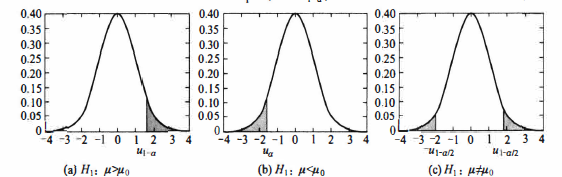
\includegraphics{figures/fig721.png}
\end{figure}
下面我们讲述用p值进行检验的方法.
类似于7.1.3节的讲述,对给定的样本观测值,可以计算出相应的检验统计量$\mu$的值,记$u_{0}=\frac{\sqrt{n}\left(\overline{x}-\mu_{0}\right)}{\sigma_{0}}$这里的$\overline{x}$是样本观测值.因在$\mu=\mu_{0}$时,$u$是服从标准正态分布的随机变量,令
\begin{equation}p_{1}=P(u\geq u_{0})=1-\Phi(u_{0})\end{equation}
此即说明$u_{0}=u_{1-p_{1}}$,于是由正态分布函数的反函数的单调性有如下结论:
\begin{itemize}
    \item 当$p_{1}\leqslant\alpha$时,$u_{1-\alpha}\leq u_{_0}$,于是观测值落在拒绝域里,应拒绝原假设。
    \item 当$p_{1}>\alpha$时,$u_{1-\alpha}>u_{0}$,于是观测值不在拒绝域里,应接受原假设.
\end{itemize}
由此可以看出,上式计算出的值就是该检验的$p$值.

对检验问题(7.2.2)所示的单侧检验问题2的讨论是完全类似的,仍选用$\mu$作为检验统计量,考虑到(7.2.2) 的备择假设$H_1$在左侧,其拒绝域为
\begin{equation}
    W_{2}=\{u\leq u_{_\alpha}\}.
\end{equation}
而检验的p值为
\begin{equation}p_{2}=P(u\leq u_0)=\Phi(u_0),\end{equation}
对检验间题(7.2.3)所示的双侧检验问题3,也可类似进行讨论,只不过检验的$p$值稍有不同仍选用$\mu$作为检验统计量,考虑到(7.2.3)的备择假设几分散在两侧,故其拒绝域亦应在两侧,即拒绝域应有如下形式
$$W_3=\{|u|\geqslant c\}$$
对给定的显著性水平$\alpha (0<\alpha<1)$,由$P_{\mu_{0}}(|u\mid\geq c)=\alpha $可定出$c=\mu_{1-\alpha/2}$最后的拒绝域为
\begin{equation}
    W_3=\{|u|\geqslant \mu_{1-\alpha/2}\}
\end{equation}
下面介绍双侧检验的$p$值的计算.在检验统计量分布对称场合,双侧检验的$p$值的计算与单侧检验是类似的,不对称场合我们在后面介绍.

仿上,令
\begin{equation}P_{3}=P(|u|\geqslant|u_{_0}|)=2(1-\Phi(|u_{_0}|)),\end{equation}
此即说明$|u_{_0}|=\mu_{1-p_{3}/2}$,这里要用到$\mu_0$的绝对值是因为对双侧假设检验,观测值可能为正,也可能为负,二者机会相同,于是有类似的结论:
\begin{itemize}
    \item 当$p_3 \leq \alpha$时,$\mu_{1-\alpha/2} \leq |\mu_0|$,于是观测值落在拒绝域里,应拒绝原假设.
    \item 当$p_3 > \alpha$时,$\mu_{1-\alpha/2} > |\mu_0|$,于是观测值不在拒绝域里,应接受原假设.
\end{itemize}

\paragraph{二、$\sigma$未知时的$t$检验}~{}

对检验问题I,由于$\sigma$ 未知,无法使用(7.2. 4)式作检验.一个自然的想法是将(7.2.4)式中未知的$\sigma$替换成样本标准差$s$,这就形成$t$检验统计量
\begin{equation}
    t = \frac{\sqrt{n}(\bar{x}-\mu_0)}{s}
\end{equation}
由推论5.4.2知,在$\mu=\mu_0$时,$t\sim t(n-1)$,从而检验问题1的拒绝域为
\begin{equation}
    W_1 = \{t \geqslant t_{1-\alpha}(n-1)\}
\end{equation}
检验的$p$值是类似的,对给定的样本观测值,可以计算出相应的检验统计量$t$的值,记为$t_0=\frac{\sqrt{n}(\bar{x}-\mu_0)}{s}$,,这里的$\bar{x},s$可由样本观测值算得.因$t$服从自由度是$n-1$的$t$分布的随机变量,则
\begin{equation}
    p_1 = P(t \geqslant t_0)
\end{equation}
对另两组检验问题的讨论是完全类似于上一小节的,罗列结果如下:检验问题2
的拒绝域为
\begin{equation}
    W_2 = \{t \leqslant t_{\alpha}(n-1)\}
\end{equation}
$p$值为
\begin{equation}
    p_2 = P(t \leqslant t_0)
\end{equation}
检验问题3的拒绝域为
\begin{equation}
    W_3 = \{|t| \geqslant t_{1-\alpha/2}(n-1)\}
\end{equation}
$p$值为
\begin{equation}
    p_3 = P(|t| \geqslant |t_0|)
\end{equation}



\begin{table}[H]
    \caption{单个正态总体均值的假设检验}
    \centering
    \begin{tabular}{cccccc}
        \toprule[1.5pt]
        检验法 & $H_0$            & $H_1$              & 检验统计量 & 拒绝域                               & $p$值                  \\
        \midrule[1pt]
        \multirow{3}{*}{\makecell{$u$检验                                                                                 \\($\sigma = \sigma_0$已知)}} & $\mu \leq \mu_0$  & $\mu > \mu_0$  & \multirow{3}{*}{$u=\frac{\overline{x}-\mu_0}{\sigma_0 / \sqrt{n}}$}  & $\{u \geq u_{1-\alpha}\}$  & $1-\Phi(u_0)$  \\
            & $\mu \geq \mu_0$ & $\mu_1 < \mu_0$    &       & $\{u \leq u_{\alpha}\}$           & $\Phi(u_0)$           \\
            & $\mu = \mu_0$    & $\mu_1 \neq \mu_0$ &       & $\{|u|\geq u_{1-\alpha /2}\}$     & $2(1-\Phi(|u_0|))$    \\
        \addlinespace % 插入一行空白
        \multirow{3}{*}{\makecell{$t$检验                                                                                 \\($\sigma$未知)}} & $\mu \leq \mu_0$ & $\mu > \mu_0$ & \multirow{3}{*}{$t=\frac{\overline{x}-\mu_0}{s /\sqrt{n}}$ }& $\{ t\geq t_{1-\alpha}(n-1)\}$ & $P(t\geqslant t_{0})$\\
            & $\mu \geq \mu_0$ & $\mu < \mu_0$      &       & $\{ t\leq t_{\alpha}(n-1)\}$      & $P(t\leqslant t_{0})$ \\
            & $\mu = \mu_0$    & $\mu \neq \mu_0$   &       & $\{|t|\geq t_{1-\alpha/2}(n-1)\}$ & $P(|t|\geq |t_0|)$    \\
        \bottomrule
    \end{tabular}
\end{table}
注:$u_0=\sqrt{n}(\overline{x}-\mu_0)/\sigma_0,t_0=\sqrt{n}(\overline{x}-\mu_0)/s,u$是服从$N(0,1)$的随机变量,$t$是服从$t(n-1)$的随机变量.

\subsection{假设检验与置信区间的关系}
细心的读者可能会发现,这里用的检验统计昼与6.6.3节中置信区间所用的枢轴
量很相似,这不是偶然的,两者之间存在非常密切的关系,现以标准差未知场合为例叙述如下.
设$x_{1},x_{2},\cdots,x_{n}$是来自正态总体$N(\mu,\sigma^2)$的样本,现讨论在$\sigma$未知场合关于均值$\mu$的检验问题.分三种情况:

首先考虑双侧检验问题3,显著性水平为$\alpha$的检验的接受域为
$$\overline{W}_3=\{| \overline{x}-\mu_{0}| \leq\frac{s}{\sqrt{n}}t_{1-\alpha/2}(n-1)\}$$
它可以改写为
$$
    \bar{W} = \{ \bar{x}-\frac{s}{\sqrt{n}}t_{1-\alpha/2}(n-1) \leq \mu_0 \leq \bar{x} +\frac{s}{\sqrt{n}}t_{1-\alpha/2}(n-1) \}
$$
这里$\mu$并无限制,若让$\mu_0$在$(-\infty,\infty)$内取值,就可得到$\mu$的$1-\alpha$置信区间$\left[\overline{x}\pm\frac{s}{\sqrt{n}}t_{1-a/2}(n-1)\right]$。反之,若有一个如上的$1-\alpha$置信区间,也可获得关于$H_0:\mu=\mu_0$的显著性水平为$\alpha$的显著性检验。所以,“正态均值$\mu$的$1-\alpha$置信区间”与“ 关于$H_0:\mu=\mu_0 \quad vs \quad H_1:\mu \neq \mu_0$的双侧检验问题的显著性水平为$\alpha$的检验”是一一对应的。

类似地考虑单侧检验问题I,显著性水平为$\alpha$的检验的接受域为
$$\overline{W}_{1}=\left\{\overline{x}-\mu_{0}\leqslant\frac{s}{\sqrt{n}}t_{1-\alpha}(n-1)\right\}=\left\{\mu_{0}\geqslant\overline{x}-\frac{s}{\sqrt{n}}t_{1-\alpha}(n-1)\right\}$$这就给出了参数$\mu$的$1-\alpha$置信下限.反之,对上述给定的$\mu$的$1-\alpha$置信下限,我们也可以得到关于$H_0:\mu\leq \mu_0$的单侧检验问题的显著性水平为$\alpha$的检验,它们之间也是一一
对应的同样,对单侧检验问题2,其显著性水平为$\alpha$的检验与参数$\mu$的$1-\alpha$置信上限也是一一对应的.
\subsection{两个正态总体均值差的假设检验}
设$x_{1},x_{2},\cdots,x_{m}$是来自正态总体$N(\mu_1,\sigma_1^2)$的样本,$y_{1},y_{2},\cdots,y_{n}$是来自另一个正态总体$N(\mu_2,\sigma_2^2)$的样本,两个样本相互独立考虑如下三类检验问题:
\begin{align}
    H_{0}:\mu_{1}-\mu_{2} \leq 0 \quad vs \quad H_{1}:\mu_{1}-\mu_{2}>0.      \\
    H_{0}:\mu_{1}-\mu_{2}\geqslant 0  \quad vs \quad H_{1}:\mu_{1}-\mu_{2}<0. \\
    H_{0}:\mu_{1}-\mu_{2}=0 \quad vs \quad H_{1}:\mu_{1}-\mu_{2}\neq0.
\end{align}
\paragraph{一、$\sigma_1,\sigma_2$已知时两样本$\mu$的检验}~{}

此时$\mu_1-\mu_2$的点估计$\bar{x}-\bar{y}$的分布完全已知,
$$\overline{x}-\overline{y}-N\left(\mu,-\mu_{2},\frac{\sigma_{1}^{2}}{m}+\frac{\sigma_{2}^{2}}{n}\right).$$
由此可采用u检验方法,检验统计量为
$$u=\frac{\overline{x}-\overline{y}}{\sqrt{\frac{\sigma_{1}^{2}}{m}+\frac{\sigma_{2}^{2}}{n}}}.$$
在$\mu_1=\mu_2$时,$\mu\sim N(0,1)$。检验的拒绝域取决于备择假设的具体内容.对(7.2.19)所示的检验问题1,检验的拒绝域与$p$值分别为
$$W_{1}=\{ u\geq u_{1-\alpha}\},\quad p_{1}=1-\Phi(u_{0})$$
其中$u_{0}=\frac{\overline{x}-\overline{y}}{\sqrt{\frac{\sigma_{1}^{2}}{m}+\frac{\sigma_{2}^{2}}{n}}}$是由样本计算得到的检验统计量的值.对(7.2.20)所示的检验问题2,检验的拒绝域与$p$值分别为
$$W_{2}=\{ u\leq u_{\alpha}\},\quad p_{2}=\Phi(u_{0})$$
对(7.2.21)所示的检验问题3,检验的拒绝域与$p$值分别为
$$W_{3}=\{ |u|\geq u_{1-\alpha/2}\},\quad p_{3}=2(1-\Phi(|u_{0}|))$$

\paragraph{二、$\sigma_1=\sigma_2=\sigma$但未知的两样本$t$检验}~{}

在$\sigma_1=\sigma_2=\sigma$但未知时,首先
$$\bar{x}-\bar{y}\sim N\left(\left.\mu_1-\mu_{2},\left(\frac{1}{m}+\frac{1}{n}\right)\sigma^{2}\right.\right)$$
其次,由于
$$\frac1{\sigma^2}\sum_{i=1}^m{(x_i-\overline{x})^2}\quad\sim{\mathcal X}^2(m-1),\quad\frac1{\sigma^2}\sum_{i=1}^n{(y_i-\overline{y})^2}\quad\sim{\mathcal X}^2(n-1)$$
故$\frac{1}{\sigma^{2}}(\sum(x_{i}-\overline{x})^{2}+\sum(y_{i}-\overline{y})^{2})-\chi^{2}(m+n-2)$,记
$$s_{w}^{2}=\frac{1}{m+n-2}\Big[\sum_{i=1}^{m}(x_{i}-\overline{x})^{2}+\sum_{i=1}^{n}(y_{i}-\overline{y})^{2}\Big]$$
于是有
$$t=\frac{(\overline{x}-\overline{y})-(\mu_{1}-\mu_{2})}{s_{w}\sqrt{\frac{1}{m}+\frac{1}{n}}}\sim t(m+n-2)$$
当$\mu_1=\mu_2$时,检验统计量为
$$t=\frac{\overline{x}-\overline{y}}{s_{_w}\sqrt{\frac1m+\frac1n}}$$
对检验问题1,检验的拒绝域与$p$值分别为
$$W_{1}= \{ t\geqslant t_{1-\alpha}(m+n-2)\},\quad p_{1}=P(t\geqslant t_{0})$$
其中$t_0=\frac{\overline{x}-\overline{y}}{s_{_w}\sqrt{\frac1m+\frac1n}}$是由样本计算得到的检验统计量的值,$t$是服从自由度是$n+m-2$的$t$分布的随机变量.对检验问题2,检验的拒绝域与$p$值分别为
$$W_{2}=\{ t\leq t_{\alpha}(m+n-2)\},\quad p_{2}=P(t\leq t_{0}).$$
对检验问题3,检验的拒绝域与$p$值分别为
$$W_{3}=\{ |t|\geq t_{1-\alpha/2}(m+n-2)\},\quad p_{3}=P(|t|\geq |t_{0}|).$$


\begin{table}[H]
    \caption{两个正态总体均值的假设检验}
    \centering
    \begin{tabular}{cccccc}
        \toprule[1.5pt]
        检验法 & $H_0$              & $H_1$              & 检验统计量 & 拒绝域                                 & $p$值                      \\
        \midrule[1pt]
        \multirow{3}{*}{\makecell{$u$检验                                                                                         \\($\sigma_1,\sigma_2$已知)}} & $\mu_1 \leq \mu_2$  & $\mu_1 > \mu_2$  & \multirow{3}{*}{$u=\frac{\overline{x}-\overline{y}}{\sqrt{\frac{\sigma_{_1}^2}m+\frac{\sigma_{_2}^2}n}}$}  & $\{u \geq u_{1-\alpha}\}$  & $1-\Phi(u_1)$  \\
            & $\mu_1 \geq \mu_2$ & $\mu_1 < \mu_2$    &       & $\{u \leq u_{\alpha}\}$             & $\Phi(u_1)$               \\
            & $\mu_1 = \mu_2$    & $\mu_1 \neq \mu_2$ &       & $\{|u|\geq u_{1-\alpha /2}\}$       & $2(1-\Phi(|u_1|))$        \\
        \addlinespace % 插入一行空白
        \multirow{3}{*}{\makecell{$t$检验                                                                                         \\($\sigma_1=\sigma_2$未知)}} & $\mu_1 \leq \mu_2$ & $\mu_1 > \mu_2$ & \multirow{3}{*}{$t=\frac{\overline{x}-\overline{y}}{s_{w}\sqrt{\frac1m+\frac1n}}$ }& $\{ t\geq t_{1-\alpha}(m+n-2)\}$ & $P(T_{1}\geqslant t_{1})$\\
            & $\mu_1 \geq \mu_2$ & $\mu_1 < \mu_2$    &       & $\{ t\leq t_{\alpha}(m+n-2)\}$      & $P(T_{1}\leqslant t_{1})$ \\
            & $\mu_1 = \mu_2$    & $\mu_1 \neq \mu_2$ &       & $\{|t|\geq t_{1-\alpha/2}(m+n-2)\}$ & $P(|T_1|\geq |t_1|)$      \\
        \bottomrule
    \end{tabular}
\end{table}

\begin{table}[H]
    \caption{两个正态总体均值的假设检验\label{tab:experiment1}}
    \centering
    \begin{tabular}{cccccc}
        \toprule[1.5pt]
        检验法 & $H_0$              & $H_1$              & 检验统计量 & 拒绝域                             & $p$值                      \\
        \midrule[1pt]
        \multirow{3}{*}{\makecell{大样本$u$检验                                                                                  \\($m,n$充分大)}} & $\mu_1 \leq \mu_2$  & $\mu_1 > \mu_2$  & \multirow{3}{*}{$u=\frac{\overline{x}-\overline{y}}{\sqrt{\frac{s_x^2}m+\frac{s_y^2}n}}$}  & $\{u \geq u_{1-\alpha}\}$  & $1-\Phi(u_2)$  \\
            & $\mu_1 \geq \mu_2$ & $\mu_1 < \mu_2$    &       & $\{u \leq u_{\alpha}\}$         & $\Phi(u_2)$               \\
            & $\mu_1 = \mu_2$    & $\mu_1 \neq \mu_2$ &       & $\{|u|\geq u_{1-\alpha /2}\}$   & $2(1-\Phi(|u_2|))$        \\
        \addlinespace % 插入一行空白
        \multirow{3}{*}{\makecell{近似$t$检验                                                                                   \\($m,n$不很大)}} & $\mu_1 \leq \mu_2$ & $\mu_1 > \mu_2$ & \multirow{3}{*}{$t=\frac{\overline{x}-\overline{y}}{\sqrt{\frac{s_x^2}{m}+\frac{x_y^2}{n}  }}$ }& $\{ t\geq t_{1-\alpha}(l)\}$ & $P(T_{1}\geqslant t_{2})$\\
            & $\mu_1 \geq \mu_2$ & $\mu_1 < \mu_2$    &       & $\{ t\leq t_{\alpha}(l)\}$      & $P(T_{1}\leqslant t_{2})$ \\
            & $\mu_1 = \mu_2$    & $\mu_1 \neq \mu_2$ &       & $\{|t|\geq t_{1-\alpha/2}(l)\}$ & $P(|T_1|\geq |t_2|)$      \\
        \bottomrule
    \end{tabular}
\end{table}
注:$u_{1}=\frac{\overline{x}-\overline{y}}{\sqrt{\frac{\sigma_{1}^{2}}{m}+\frac{\sigma_{2}^{2}}{n}}}$,$u_{2}=\frac{\overline{x}-\overline{y}}{\sqrt{\frac{s_{x}^{2}}{m}+\frac{s_{y}^{2}}{n}}}$,$t_{1}=\frac{\overline{x}-\overline{y}}{s_{w}\sqrt{\frac{1}{m}+\frac{1}{n}}}$,$t_{2}=\frac{\overline{x}-\overline{y}}{\sqrt{\frac{s_{x}^{2}}{m}+\frac{s_{y}^{2}}{n}}}$,$T_1$是服从自由度为$n+m-2$的$t$分布的随机变量, $T_2$是服从自由度为$l$的$t$分布的随机变量, $l$与$s_w$的表达式见6.6.6 节
\subsection{成对数据检验}
在对两个总体均值进行比较时, 有时数据是成对出现的,此时若采用二样本t检验所得出的结论有可能是不对的,下面看一个例子.
\subsection{正态总体方差的检验}
\paragraph{一、单个正态总体方差的$\chi^2$检验}~{}
设$x_{1},x_{2},\cdots,x_{m}$是来自正态总体$N(\mu,\sigma^2)$的样本,对方差亦可考虑如下三个检验问题:
\begin{align}
    H_{0}:\sigma^{2}\leq\sigma_{0}^{2} \quad vs \quad H_{1}:\sigma^{2}>\sigma_{0}^{2}. \\
    H_{0}:\sigma^{2}\geq\sigma_{0}^{2} \quad vs \quad H_{1}:\sigma^{2}<\sigma_{0}^{2}. \\
    H_{0}:\sigma^{2}=\sigma_{0}^{2} \quad vs \quad H_{1}:\sigma^{2}\neq\sigma_{0}^{2}.
\end{align}
其中$\sigma_0$是已知常数。此处通常假定$\mu$未知,它们采用的检验统计量是相同的,均为
\begin{equation}\mathcal {X}^{2}=\left({n-1}\\ \right)s^{2}/\sigma_{0}^{2}.\end{equation}
在$\sigma^2=\sigma_0^2$时,$\chi^2\sim \chi^2(n-1)$,于是,若取显著性水平为$\alpha$,则对应三个检验间题的显著性水平为$\alpha$的检验的拒绝域依次为
$$
    \begin{aligned}
        W_{1} & =\{\chi^{2}\geq\chi_{1-\alpha}^{2}(n-1)\},                                                           \\
        W_{2} & =\{\chi^{2}\leq\chi_{\alpha}^{2}(n-1)\},                                                             \\
        W_{3} & =\{\chi^{2}\leq\chi_{\alpha/2}^{2}(n-1)\quad\text{or}\quad\chi^{2} \geq \chi_{1-\alpha/2}^{2}(n-1)\}
    \end{aligned}
$$

我们亦可给出检验的$p$值.对单侧检验,想法是类似的,记 ${\mathcal X}_{0}^{2}=(n-1)s^{2}/\sigma_{0}^{2}$是由样本计算得到的检验统计量的值,$\chi^2$表示服从自由度为$n-1$的$\chi^2$分布的随机变量,则检
验问题1, 2的$p$值分别为$p_1=P(\chi^2 \geq \chi_0^2)$,$p_2 = P(\chi^2 \leq \chi_0^2)$。对双侧检验则稍稍复杂一
点,事实上,双侧检验的拒绝域在两侧,用$\chi_0^2$可算得两个尾概率$P(\chi^2 \leq \chi_0^2)$和$P(\chi^2 \geq \chi_0^2)$,其和为1 ,其中必有一个$\leq 0.5$.检验的注意力总放在拒绝域上,故应从中选一个小
的与$\alpha / 2$比较,从而检验问题3的$p$值为
\begin{equation}
    p_3 = 2\min\{P(\chi^2 \leq \chi_0^2),P(\chi^2 \geq \chi_0^2)\}
\end{equation}
对这样定义的p值,不难发现下述结论仍然是成立的:


\begin{itemize}
    \item 当$p_3 \leq \alpha$时,应拒绝原假设
    \item 当$p_3 > \alpha$时,应接受原假设
\end{itemize}

\paragraph{二、两个正态总体方差比的$F$检验}~{}

设$x_{1},x_{2},\cdots,x_{m}$是来自$N(\mu_1,\sigma_1^2)$的样本,$y_{1},y_{2},\cdots,y_{n}$是来自$N(\mu_2,\sigma_2^2)$的样本,考虑如下三个假设检验问题:
\begin{align}
    H_{0}:\sigma_{1}^{2} \leq \sigma_{2}^{2} \quad vs \quad H_{1}:\sigma_{1}^{2}>\sigma_{2}^{2}. \\
    H_{0}:\sigma_{1}^{2} \geq \sigma_{2}^{2} \quad vs \quad H_{1}:\sigma_{1}^{2}<\sigma_{2}^{2}. \\
    H_{0}:\sigma_{1}^{2}=\sigma_{2}^{2} \quad vs \quad H_{1}:\sigma_{1}^{2}\neq\sigma_{2}^{2}.
\end{align}
此处$\mu_1,\mu_2$均未知,记$s_x^2,s_y^2$分别是由$x_1,x_2,\cdots,x_m$算得的$\sigma^1$的无偏估计和由$y_1,y_2,\cdots,y_n$算得的$\sigma^2$的无偏估计,即(两个都是样本方差),则可建立如下的检验统计量:
\begin{equation}
    F = \frac{s_x^2}{s_y^2}
\end{equation}
当$\sigma_1=\sigma_2$时,$F\sim F(m-1,n-1)$,由此给出三个检验问题对应的拒绝域依次为:
$$
    \begin{aligned}
        W_{1} & =\{F\geq F_{1-\alpha}(m-1,n-1)\},                                                 \\
        W_{2} & =\{F\leq F_{\alpha}(m-1,n-1)\},                                                   \\
        W_{3} & =\{F\leq F_{\alpha/2}(m-1,n-1)\quad\text{or}\quad F\geq F_{1-\alpha/2}(m-1,n-1)\}
    \end{aligned}
$$
此时检验的$p$值的讨论与前述$\chi^2$是相似的,记$F_0=s_x^2/s_y^2$,是由样本计算得到的检验统计量的值,$F$表示服从$F(m-1,n-1)$分布的随机变量,则检验问题1,2,3的$p$值分别为
$$
    \begin{aligned}
        p_1 & =P(F\geq F_0),                      \\
        p_2 & =P(F\leq F_0),                      \\
        p_3 & =2\min\{P(F\geq F_0),P(F\leq F_0)\}
    \end{aligned}
$$

\begin{table}[H]
    \caption{正态总体方差的假设检验}
    \centering
    \begin{tabular}{cccccc}
        \toprule[1.5pt]
        检验法                         & $H_0$                        & $H_1$                        & 检验统计量                                                   & 拒绝域                                              & $p$值                      \\
        \midrule[1pt]
        \multirow{3}{*}{$\chi^2$检验} & $\sigma^2 \leq \sigma_0^2$   & $\sigma^2 > \sigma_0^2$      & \multirow{3}{*}{$\chi^2=\frac{(n - 1)s^2}{\sigma_0^2}$} & $\chi^2 \geq \chi_{1-\alpha}^2(n-1)$             & $P(\chi^2 \geq \chi_0^2)$ \\

                                    & $\sigma^2 \geq \sigma_0^2$   & $\sigma^2 < \sigma_0^2$      &                                                         & $\chi^2 \leq \chi_{\alpha}^2(n-1)$               & $P(\chi^2 \leq \chi^2_0)$ \\

                                    & $\sigma^2 = \sigma_0^2$      & $\sigma^2 \neq \sigma_0^2$   &                                                         & \makecell{$\chi^2 \leq \chi_{\alpha /2}^2(n-1)$或                             \\$\chi^2 \geq \chi_{1-\alpha /2}^2(n-1) $} &\makecell{$2\min\{P(\chi^{2}\leq \chi_{0}^{2}),$\\$P(\chi^{2}\geq \chi_{0}^{2})\}$}\\
        \midrule
        \multirow{3}{*}{$F$检验}      & $\sigma_1^2 \leq \sigma_2^2$ & $\sigma_1^2 > \sigma_2^2$    & \multirow{3}{*}{$F=\frac{s_x^2}{s_y^2}$}                & $F \geq F_{1-\alpha}(m-1,n-1)$                   & $P(F \geq F_0)$           \\

                                    & $\sigma_1^2 \geq \sigma_2^2$ & $\sigma_1^2 < \sigma_2^2$    &                                                         & $F \leq F_{\alpha}(m-1,n-1)$                     & $P(F \leq F_0)$           \\

                                    & $\sigma_1^2 = \sigma_2^2$    & $\sigma_1^2 \neq \sigma_2^2$ &                                                         & \makecell{$F\leq F_{\alpha/2}(m-1,n-1)$或                                     \\$F \geq F_{1-\alpha/2}(m-1,n-1)$} &\makecell{$2\min\{P(F\leq F_0),$\\ $P(F \geq F_0)\}$} \\
        \bottomrule
    \end{tabular}
\end{table}
\section{其他分布参数的假设检验}
\subsection{指数分布参数的假设检验}
指数分布是一类重要的分布,有广泛的应用.设$x_1,x_2,\cdots,x_n$是来自指数分布$Exp(1/\theta)$的样本,$\theta$为其均值,现考虑关于$\theta$的如下检验问题:
\begin{equation}
    H_0:\theta \leq \theta_0 \quad vs \quad H_1:\theta > \theta_0
\end{equation}
为寻找检验统计量, 我们考察参数$\theta$的充分统计量$\bar{x}$,在$\theta=\theta_0$时,$n \bar{x}=\sum_{i=1}^nx_i\sim Ga(n,1/\theta_0)$,由伽马分布性质可知
\begin{equation}
    \chi^2=\frac{2n\bar{x}}{\theta_0}\sim \chi^2(2n)
\end{equation}
于是可用$\chi^2$作为检验统计量并利用$\chi^2(2n)$的分位数建立检验的拒绝域,对检验问题(7.3. l),拒绝域形式为$W_1=\{\chi^2 \geq c\}$,对给定的显著性水平$\alpha$,可由$P(W_1)=\alpha$获得拒绝域如下:
\begin{equation}
    W_1=\{\chi^2 \geq \chi_{1-\alpha}^2(2n)\}
\end{equation}
类似本章前面关于检验的$p$值的讨论,记${\mathcal X}_{0}^{2}=\frac{2n\overline{x}}{\theta_{0}}$为由样本算得的检验统计量值,$\chi^2$表示服从$\chi^2(2n)$分布的随机变量,则检验的$p$值为$p_1=P(\chi^2 \geq \chi_0^2)$

关于0的另两种检验间题处理方法类似.对检验问题
$$
    2\quad H_0:\theta \geq \theta_0 \quad vs \quad H_1:\theta < \theta_0 \quad \text{and} \quad 3 \quad H_0:\theta = \theta_0 \quad vs \quad H_1:\theta \neq \theta_0
$$
检验统计量不变,拒绝域以及检验的$p$值分别为
$$
    \begin{aligned}
        W_2 & = \{\chi^2 \leq \chi_{\alpha}^2(2n)\}, \quad p_2 = P(\chi^2 \leq \chi_0^2)                                                                                              \\
        W_3 & = \{\chi^2 \leq \chi_{\alpha/2}^2(2n) \quad \text{or} \quad \chi^2 \geq \chi_{1-\alpha/2}^2(2n)\}, \quad p_3 = 2\min\{P(\chi^2 \geq \chi_0^2),P(\chi^2 \leq \chi_0^2)\}
    \end{aligned}
$$

\begin{table}[H]
    \caption{指数分布均值$\theta$的假设检验}
    \centering
    \begin{tabular}{cccccc}
        \toprule[1.5pt]
        检验法                         & $H_0$                        & $H_1$                        & 检验统计量                                                   & 拒绝域                                              & $p$值                      \\
        \midrule[1pt]
        \multirow{3}{*}{$\chi^2$检验} & $\theta \leq \theta_0$   & $\theta > \theta_0$      & \multirow{3}{*}{$\chi^2=\frac{2n \overline{x}}{\theta_0}$} & $\chi^2 \geq \chi_{1-\alpha}^2(2n)$             & $P(\chi^2 \geq \chi_0^2)$ \\

        & $\theta \geq \theta_0$   & $\theta< \theta_0$      &                                                         & $\chi^2 \leq \chi_{\alpha}^2(2n)$               & $P(\chi^2 \leq \chi^2_0)$ \\

        & $\theta= \theta_0$      & $\theta \neq \theta_0$   &                                                         & \makecell{$\chi^2 \leq \chi_{\alpha /2}^2(2n)$或 \\
        $\chi^2 \geq \chi_{1-\alpha /2}^2(2n) $} &\makecell{$2\min\{P(\chi^{2}\leq \chi_{0}^{2}),$\\$P(\chi^{2}\geq \chi_{0}^{2})\}$}\\
        \bottomrule
    \end{tabular}
\end{table}
\subsection{比率p的检验}
比率$p$可看作某事件发生的概率,即可看作二点分布$b(1,p)$中的参数,作$n$次独立试验,以$x$记该事件发生的次数,则$x \sim b(n,p)$。我们可以根据$x$检验关于$p$的一些假设。考虑如下单边假设检验问题:
\begin{equation}
    1 \quad H_0:p \leq p_0 \quad vs \quad H_1:p > p_0
\end{equation}
直观上看,一个显然的检验方法是取如下的拒绝域$W=\{x\geq c\}$,由于$x$只取整数值,故$c$可限制在非负整数中然而,一般情况下对给定的$\alpha$,不一定能正好取到一个c,使得
\begin{equation}
    P(x \geq c;p_{_0}) = \sum_{i=c}^{n}\tbinom{n}{i}p_{_0}^i(1-p_{_0})^{n-i} = \alpha
\end{equation}
能恰巧使得(7.3 .5)成立的$c$值是罕见的.这是在对离散总体作假设检验中普遍会遇到的问题,在这种情况下,较常见的是找一个$C_0$,使得
$$\sum_{i=c_0}^n\binom{n}{i}p_0^i(1-p_0)^{n-i}>\alpha>\sum_{i=c_0+1}^n\binom{n}{i}p_0^i(1-p_0)^{n-i}.$$
于是,可取$c=c_{_0}+1$此时相当于把显著性水平由$\alpha$降低到$\sum_{i=c_0+1}^n{\binom ni}p_0^i(1-p_0)^{n-i}$因为它可保证(7.3 .5)的左侧不大于$\alpha$,从而是显著性水平为$\alpha$的检验.

事实上,在离散场合使用$p$值作检验较为简便, 这时可以不用找$C_{_0}$,而只需根据观测值$x=x_{_0}$计算检验的$p$值,即
$$
    p = P(x \geq x_0)
$$

对另两个检验问题的处理是类似的.检验问题2$H_0:p \geq p_0 \quad vs H_1:p<p_0$以及检验问题3$H_0:p=p_0 \quad vs \quad H_1:p \neq p_0$的$p$值分别为
$$
    p_2 = P(x \leq x_0),
    p_3 = 2\min\{P(x \leq x_0),P(x \geq x_0)\}
$$


\begin{table}[H]
    \centering
    \caption{小样本比例$p$的假设检验}
    \begin{tabular}{@{}ccc@{}}
    \toprule
   $H_0$ & $H_1$ &$p$值\\ 
   \midrule
   $p \leq p_0$  &  $p \geq p_0$ & $P(x \geq x_0)$ \\
   $p \geq p_0$ &  $p \leq p_0$ & $P(x\leq x_0)$ \\ 
   $p = p_0$&  $p \neq p_0$&$ 2 \min \{P(x\leq x_0),P(x \geq x_0)\}$ \\
   \bottomrule
    \end{tabular}
\end{table}
\subsection{大样本检验}
在实际使用中,如果样本量较大,人们还经常采用渐近正态分布构
造检验统计量,获得大样本检验.其一般思路如下:设$x_1,x_2,\cdots,x_n$是来自某总体$F(x;\theta)$的样本,又设该总体均值为$\theta$,方差为$\theta$的函数,记为$\sigma^2(\theta)$.对二点分布$b(1,\theta)$,其方差$\sigma^2(\theta)=\theta(1-\theta)$,现要对下列三类假设检验问题:
\begin{align}
    1\quad H_0:\theta \leq \theta_0 \quad vs \quad H_1:\theta > \theta_0 \\
    2\quad H_0:\theta \geq \theta_0 \quad vs \quad H_1:\theta < \theta_0 \\
    3\quad H_0:\theta = \theta_0 \quad vs \quad H_1:\theta \neq \theta_0
\end{align}
寻找大样本检验方法. 在样本容量$n$充分大时,利用中心极限定理知$\bar{x} \dot\sim N(\theta,\sigma^2(\theta)/n)$,故在$\theta=\theta_0$时,可采用如下检验统计量:
\begin{equation}
    u=\frac{\sqrt{n}\left(\overline{x}-\theta_{0}\right)}{\sqrt{\sigma^{2}(\hat{\theta})}}\dot{\sim}N(0,1)
\end{equation}
其中$\hat{\theta}$为$\theta$的$MLE$,并由此可近似地确定拒绝域. 对应上述三类检验问题的拒绝域依次为
$$
    \begin{aligned}
        W_1 & = \{u \geq u_{1-\alpha}\},      \\
        W_2 & = \{u \leq u_{\alpha}\},        \\
        W_3 & = \{|u| \geq u_{1- \alpha /2}\}
    \end{aligned}
$$
检验的近似的$p$值也是可以计算的,与单样本正态总体场合完全一样,此处从略.


\begin{table}[H]
    \centering
    \caption{大样本比例$p$的假设检验}
    \begin{tabular}{@{}cccc@{}}
    \toprule
   $H_0$ & $H_1$ &拒绝域 &$p$值\\ 
   \midrule
   $p \leq p_0$  &  $p > p_0$&  $\{u\geq u_{1-\alpha} \}$& $1-\Phi(u_0)$ \\
   $p \geq p_0$ &  $p < p_0$ &$\{ u \leq u_{\alpha}\} $& $\Phi(u_0) $ \\ 
   $p = p_0$&  $p \neq p_0$&$\{ |u| \geq u_{1-\alpha/2} \}$ &$ 2(1-\Phi(|u_0|)) $ \\
   \bottomrule
    \end{tabular}
\end{table}
\section{似然比检验与分布拟合检验}
\subsection{似然比检验的思想}
\begin{definition}
    设$x_{1},x_{2},\cdots,x_{n}$为来自密度函数为$p(x;\theta),\theta \in \Theta$的总体的样本,考虑如下检验问题:
    \begin{equation}
        H_{0}:\theta \in \Theta_{0} \quad vs \quad H_{1}:\theta \in \Theta_{1}=\Theta-\Theta_0
    \end{equation}
    令
    \begin{equation}
        \Lambda(x_{1},x_{2},\cdots,x_{n})=
        \frac{\sup_{\theta\in\theta}p(x_{1},x_{2},\cdots,x_{n};\theta)}
        {\sup_{\theta\in\theta_{0}}p(x_{1},x_{2},\cdots,x_{n};\theta)}
    \end{equation}
    则我们称统计量$\Lambda(x_{1},x_{2},\cdots,x_{n})$为假设(7.4.1)的似然比(likelihood ratio),有时也称之为\textbf{广义似然比}
\end{definition}
(7.4.2)式的$\Lambda(x_{1},x_{2},\cdots,x_{n})$也可以写成如下形式:
\begin{equation}
    \Lambda(x_{1},x_{2},\cdots,x_{n})=
    \frac{p(x_{1},x_{2},\cdots,x_{n};\hat{\theta})}
    {p(x_{1},x_{2},\cdots,x_{n};\hat{\theta_0})}
\end{equation}
其中$\hat{\theta}$表示在全参数空间$\Theta$上$\theta$的最大似然估计,$\hat{\theta_0}$表示在子空间$\Theta_0$上$\theta$的最大似然估计。也就是说$\Lambda(x_{1},x_{2},\cdots,x_{n})$的分子表示没有假设时的似然函数最大值, 分母表示在原假设成立条件下的似然函数最大值,不难看出,如果$\Lambda(x_{1},x_{2},\cdots,x_{n})$的值很大,则说明$\theta \in \Theta_0$的可能性要比$\theta \in \Theta_1$的可能性小,于是,我们有理由认为$H_0$不成立。这样,我们有如下的似然比检验。

\begin{definition}
    当采用(7.4. 3)式的似然比统计量$\Lambda(x_{1},x_{2},\cdots,x_{n})$作为检验问题(7.4.1) 的检验统计蜇,且取其拒绝域为$W=\{\Lambda(x_1,x_2,\cdots,x_n)\geq c\}$,其中临界值$c$满足
    \begin{equation}
        P_{\theta}(\Lambda(x_{1},x_{2},\cdots,x_{n})\geq c) \leq \alpha,\quad \forall \theta \in \Theta_0
    \end{equation}
\end{definition}
则称此检验为显著性水平$\alpha$的似然比检验(likelihood ratio test) ,简记为LRT.
\subsection{分类数据的\texorpdfstring{$ \chi^2$}{χ2}拟合优度检验}
我们对总体分布的形式建立假设并进行检验,这一类检验问题统称为分布的拟合检验,它们是一类非参数检验问题。

\begin{example}
    在19世纪, 孟德尔(Mendel)按颜色与形状把豌豆分为四类:黄圆、绿圆、黄皱和绿皱.孟德尔根据遗传学原理判断这四类的比例应为$9:3:3:1$为做验证,孟德尔在一次豌豆实验中收获了$n= 556$个豌豆,其中这四类豌豆的个数分别为$315,108,101,32$该数据是否与孟德尔提出的比例吻合?
\end{example}
这一例子是属于分类数据的检验问题,它的一般情形为:根据某项指标,总体被分成$r$类:$A_1,A_2,\\ \cdots,A_r$此时我们最关心的是关于各类元素在总体中所占的比率的假设

\begin{equation}
    \label{eq:7.4.5}
    H_0:A_i \text{所占比率是}p_{i0},i=1,2,\cdots,r
\end{equation}
其中$p_{i0}$已知。$\sum_{i=1}^{r} p_{i0}=1$.记$x_1,x_2,\cdots,x_n$为从此总体抽出的样本,且以$n_i$记这$n$个样本中属于$A_i$的样本个数。由于当$H_0$成立时,在$n$个样本中属于$A_i$类的"理论个数"
或”"期望个数"为$np_{i0}$而我们实际观测到的值为$n_i$,,故当$H_0$成立时,$n_i$与$np_{i0}$应相差不大.于是,k.皮尔逊提出用统计量
\begin{equation}
    \label{eq:7.4.6}
    {\mathcal X}^{2}=\sum_{i=1}^{r}\frac{(n_{i}-np_{i0})^2}{np_{i0}}.
\end{equation}
来衡量"理论个数"与实际个数间的差异.
在\eqref{eq:7.4.6}式中,分子$(n_{i}-np_{i0})^2$是实际观测数与期望观测数的偏差的平方,而$\frac{(n_{i}-np_{i0})^2}{np_{i0}}$可以看成是$(n_{i}-np_{i0})^2$的规范化,所以\eqref{eq:7.4.6}式提供了实际观测数与期望观测数接近程度的一个度量,当$H_0$为真时, 它的值应该比较小,所以,其拒绝域为$\{{\mathcal X}^{2} \geq c\}$,其中$c$为待定的临界值

为了控制上述检验的第一类错误,我们必须知道此检验统计量在原假设成立下的分布,为此,k.皮尔逊证明了如下定理:
\begin{theorem}
    \label{th:7.4.1}
    在前述各项假定下,在$H_0$成立时,对\eqref{eq:7.4.6}式的检验统计量有$${\mathcal X}^{2} \xrightarrow{L} {\mathcal X}^{2}(r-1).$$
\end{theorem}
根据定理\ref{th:7.4.1},对于假设\eqref{eq:7.4.5},我们可以采取如下的显著性水平近似为$\alpha$的显著性检验:检验统计量如\eqref{eq:7.4.6}所示,拒绝域为
$$
    W = \{{\mathcal X}^{2}\geq {\mathcal X}^{2}_{1-\alpha}(r-1) \}
$$
这就是K皮尔逊提出的最早的一个检验方法,通常称之为皮尔逊${\mathcal X}^{2}$拟合优度检验.

顺便指出,在某些场合,我们也可从似然比检验得到皮尔逊${\mathcal X}^{2}$拟合优度检验统计量事实上,此时样本联合分布为
$$P_{\theta}(X_{1}=x_{1},X_{2}=x_{2},\cdots,X_{n}=x_{n})=p_{1}^{n_{1}}p_{2}^{n_{2}}\cdots p_{n}^{n_r}=\prod_{i=1}^{r}p_{i}^{n_{i}},$$
由此可求得
$$
    \begin{aligned}
        \sup_{\theta \in \Theta}P_{\theta}(X_{1}=x_{1},X_{2}=x_{2},\cdots,X_{n}=x_{n})     & =\prod_{i=1}^{r}\left(\frac{n_{i}}{n}\right)^{n_{i}}, \\
        \sup_{\theta \in \Theta_{0}}P_{\theta}(X_{1}=x_{1},X_{2}=x_{2},\cdots,X_{n}=x_{n}) & =\prod_{i=1}^{r}p_{i0}^{n_{i}}
    \end{aligned}
$$
于是,其似然比统计量为
$$\Lambda(x_{1},x_{2},\cdots,x_{n})=\prod_{i=1}^{r}\left(\frac{n_{i}}{n p_{i0}}\right)^{n_{i}}.$$
有
$$2\ln A(x_{1},x_{2},\cdots,x_{n})\approx\sum_{i=1}^{r}\frac{(n_{i}-np_{i0})^{2}}{np_{i0}},$$
由单调性,此处似然比检验与皮尔逊引进的${\mathcal X}^2$拟合优度检验等价.

关于皮尔逊统计量的进一步应用,有下面几点值得注意:
\begin{enumerate}
    \item 在上面的讨论中,我们假定第$i$类$A_i$,出现的概率为$p_{i0}$都是已知的,但是,在实际问题中,有时诸$p_{i0}$还依赖于$k$个未知参数,而这$k$个未知参数需要利用样本来估计,这种情况下,k.皮尔逊建立的定理7.4.1不再成立.不过,1924年费希尔证明了,在同样的条件下,可以先用最大似然估计方法估计出这$k$个未知参数,然后再算出$p_{i0}$的估计值$\hat{p_i}(i=1,2,\cdots,r)$.这时,类似于\eqref{eq:7.4.6}式的统计量
          \begin{equation}
              \label{eq:7.4.7}
              {\mathcal X}^{2}=\sum_{i=1}^{r}\frac{(n_{i}-n \hat{p_{i}})^2}{n \hat{p_{i}}}.
          \end{equation}
          当$n \to \infty$时,还是渐近服从${\mathcal X}^2$分布,不过自由度为$r-k-1$.
    \item 无论是\eqref{eq:7.4.6}式还是\eqref{eq:7.4.7}式,因为用的是渐近分布,所以,对样本大小$n$有一定要求因此,这种${\mathcal X}^2$检验法主要用于大样本场合.这一要求体现在实际应用中,一般要求各类的观测数均不小于$5$,因此,往往需要把一些相邻的类合并达到要求.
    \item 上述拟合优度检验就是在大样本场合的多项分布检验,但对其他分布亦可提供一种分布检验方法.
\end{enumerate}

\subsection{分布的\texorpdfstring{$ \chi^2$}{χ2}拟合优度检验}
设$x_1,x_2,\cdots,x_n$是来自总体$F(x)$的样本,有时,需要检验的原假设是
$$
    H_{0}:F(x)=F_{0}(x),
$$
其中$F_0(x)$称为理论分布,它可以是一个完全已知的分布,也可以是一个仅依赖于有限个实参数且分布形式已知的分布函数.这个分布检验问题就是检验观测数据是否与理论分布相符合.在样本容量较大时,这类问题可以用$ \chi^2$拟合优度检验来解决.

\paragraph{一 总体X为离散分布}~{}

设总体$X$为取有限或可列个值$a_1,a_2,...$的离散随机变量,我们把相邻的某些$a_i$合并为一类,使得$a_1,a_2,...$被分为有限个类$A_1,A_2,...,A_r$,并使得样本观测值$x_1 ,x_2,\cdots,x_n$落入每一个$A_i$内的个数 $n_i$不小于$5$.记 $P(X\in A_i)=p_i(i=1,2,\cdots,r)$ ,那么,假设$H_{0}:$总体分布$F(x)=F_{0}(x)$就转化为如下假设:
$$
    H_{0}:A_{i}\text{所占的比例为}p_{i}(i=1,2,\cdots,r).
$$
这样,离散分布的拟合检验与前述分类数据的检验问题就完全一样了.

\paragraph{二 总体X为离散分布}~{}
设总体$X$为连续随机变量,分布函数为$F_0(x)$,这种情况略为复杂一些.一般采用下列方法:选$r-1$个实数$a_1<a_2<\cdots<a_{r-1}$,将实数族分为$r$个区间

$$
    (-\infty,a_1],(a_1,a_2],\cdots,(a_{r-1},\infty]
$$
当观测值落人第$i$个区间内,就把它看作属于第$i$类,因此,这$r$个区间就相当于$r$个类.在$H_{0}$为真时,记
$$
    p_i = P(a_{i-1} < X \leq a_i) = F_0(a_i)-F_0(a_{i-1}) ,i=1,2,\cdots,r
$$
其中$a_0=-\infty,a_r=\infty$,以$n_i$表示样本的观测值$x_1,x_2,\cdots,x_n$落入区间$(a_{i-1},a_i]$内的个数$(i=1,2,...,r)$,接下来的做法就与总体只取有限个值的情况一样了。
\subsection{列联表的独立性检验}
一般,若总体中的个体可按两个属性$A$与$B$分类,$A$ 有$r$个类$A_1,A_2,\cdots,A_r,B$ 有 $c$ 个类$B_1,B_2,\cdots,B_{c}$,从总体中抽取容量大小为$n$ 的样本,设其中有$n_{ij}$个个体既属于类$A_i$ 又属于类$B_j,n_{ij}$称为频数,将$r\times c$个$ n_{ij}$排列为一个$r$行$c$列的二维列联表,简称$r\times c$列联表.


列联表分析的基本问题是,考察各属性之间有无关联,即判别两属性是否独立.如在前例中,问题是:色盲与其性别是否有关? 在$r \times c$列联表中,若以$p_{i\cdot},\cdots,p_{\cdot j},i=1,2,\cdots,r,j=1,2,\cdots,c$和$p_{ij}$分别表示总体中的个体仅属于$A_{i}$,仅属于$B_{j}$和同时属于$A_i$ 与$B_j$的概率,可得一个二维离散分布表(表 7.4.4) ,则“$A$ ,$B$ 两属性独立"的假设可以表述为
$$
    H_{0}:p_{ij}=P_{i \cdot} P_{\cdot j},\quad i=1,2,\cdots,r,j=1\:,2,\cdots,c.
$$
这里诸$p_{ij}$共有$rc$个参数,在原假设$H_0$成立时, 这$rc$个参数$p_ij$由$r+c$个参数$p_{1\cdot},\cdots,p_{r\cdot}$和$p_{\cdot 1},\cdots,p_{\cdot c}$决定。在这后$r+c$个个参数中存在两个约束条件:$\sum_{i=1}^{r} p_{i \cdot }=1,\sum_{j=1}^{c} p_{\cdot j}=1$
所以,此时$p_{ij}$实际上由$r + c-2$个独立参数所确定。据此,检验统计量为
$$
    \chi^{2}=\sum_{i=1}^{r}\sum_{j=1}^{c}\frac{(n_{ij}-n\hat{p}_{ij})^{2}}{n\hat{p}_{ij}}
$$

% \section{正态性检验}
% \subsection{正态概率图}
% \subsection{W检验}
% \subsection{EP检验}
% \section{非参数检验}
% \subsection{游程检验}
% \subsection{符号检验}
% \subsection{秩和检验}
\chapter{方差分析与回归分析}
% \section{方差分析}
% \section{多重比较}
% \section{方差性检验}
\setcounter{section}{3}
\section{一元线性回归}
\subsection{变量间的两类关系}
回归分析处理的是变量与变量间的关系.变蜇间常见的关系有两类:一类称为\textbf{确定性关系}:这些变量间的关系是完全确定的,可以用函数$y=f(x)$来表示,$x$ (可以是向量)给定后,$y$的值就唯一确定了.另一类称为\textbf{相关关系}: 变量间有关系,但是不能用函数来表示.
\subsection{一元线性回归模型}
设$y$与$x$间有相关关系,称$x$为自变量(预报变量),$y$为因变量(响应变量),在知道$x$取值后,$y$的取值并不是确定的,它是一个随机变量,因此有一个分布,这个分布是在知道$x$的取值后$Y$的条件密度函数$p(y|x)$,我们关心的是$y$的均值$E(Y|x)$,它是$x$的函数,这个函数是确定性的:
\begin{equation}
    f(x)=E\left(Y|x\right)=\int_{-\infty}^{\infty}yp(y|x)\mathrm{d}y.
\end{equation}
这便是$y$关于$x$的回归函数一条件期望,也就是我们要寻找的相关关系的表达式.

以上的叙述是在$x$与$y$均为随机变量场合进行的,这是一类回归问题.实际中还有第二类回归问题,其自变量$x$是可控变量(一般变量),只有$y$是随机变量,它们之间的相关关系可用下式表示:
$$
    y = f(x)+\varepsilon
$$
其中$\varepsilon$是随机误差,一般假设$\varepsilon \sim N(0,\sigma^2)$.由于$\varepsilon$的随机性,导致$y$是随机变量.

常用的一元线性回归的统计模型

\begin{equation}
    \begin{cases}
        y_i=\beta_0+\beta_1x_i+\varepsilon_i,\quad i=1,2,\cdots,n, \\
        \text{各 }\varepsilon_i\text{独立同分布},\text{其分布为}N(0,\sigma^2).
    \end{cases}
\end{equation}
由数据$(x_{i},y_{i})(i=1,2,\cdots,n)$可以获得$\beta_0,\beta_1$的估计$\hat{\beta}_0,\hat{\beta}_1$,称
\begin{equation}
    \hat{y}=\hat{\beta}_0+\hat{\beta}_1x
\end{equation}
为$y$关于$x$的经验回归函数,简称为回归方程,其图形称为回归直线.给定$x_0$后,称$\hat{y}_0=\hat{\beta}_0+\hat{\beta}_1x_0$为回归值.

\subsection{回归系数的最小二乘估计}
\subsection{回归方程的显著性检验}
在使用回归方程以前,首先应对问归方程是否有意义进行判断.什么叫回归方程有意义呢?我们知道,建立回归方程的目的是寻找$y$的均值随$x$变化的规律,即找出回归方程$E(y)=\beta_0+\beta_1x$.如果$\beta_1=0$,那么不管$x$如何变化,$E(y)$ 不随$x$的变化作线性变化,那么这时求得的一元线性回归方程就没有意义,或称回归方程不显著.如果$\beta_{1}\neq 0$,那么当$x$变化时,$E(y)$随$x$的变化作线性变化,那么这时求得的回归方程就有意义, 或称回归方程是显著的.

综上,对回归方程是否有意义作判断就是要对如下的检验问题作出判断:
\begin{equation}
    \label{eq:8.4.10}
    H_0:\beta_1=0\quad \text{vs}\quad H_1:\beta_1\neq 0.
\end{equation}
拒绝$H_0$表示回归方程是显著的.

\paragraph{一、F检验}
采用方差分析的思想,我们从数据出发研究各$y_i$不同的原因.首先引入记号并称$\hat{y}_{i}=\hat{\beta}_{_0}+\hat{\beta}_{1}x_{i}$为$x_i$处的回归值,又称$y_i-\hat{y}_i$为$x_i$处的\textbf{残差}。

数据总的波动用\textbf{总偏差平方和}
$$S_{T}=\sum(y_{i}-\overline{y})^{2}=l_{yy},$$
表示.引起各$y_i$不同的原因主要有两类因素:其一是$H_0$可能不真,即$\beta_1 \neq 0$,从而$E(y)=\beta_0+\beta_1 x$随$x$变化而变化,即在每一个$x$的观测值处的回归值不同,其波动用\textbf{回归平方和}
\begin{equation}
    S_R = \sum (\hat{y}_i - \overline{y})^2
\end{equation}
表示。其二是其他一切因素,包括随机误差、$x$对$E(y)$的非线性影响等,这样在得到回归值以后,$y$的观测值与回归值之间还有差距,这可用\textbf{残差平方和}
\begin{equation}
    S_e = \sum (y_i - \hat{y}_i)^2
\end{equation}
表示。


平方和分解式:
\begin{equation}
    S_T = S_R + S_e
\end{equation}

\begin{theorem}
    设$y_1,y_2,\cdots,y_n$相互独立,且$y_i\sim N(\beta_0+\beta_1x_i,\sigma^2),i=1,2,\cdots,n$,则在上述记号下,有
    \begin{enumerate}
        \item $S_{e}/\sigma^{2} \sim \chi^{2}( n-2)$;
        \item 若$H_{0}$成立,则有$S_{R}/\sigma^{2} \sim \chi^{2}(1)$
        \item $S_R$与$S_e,\bar{y}$独立(或$\hat{\beta}_1$与$S_e,\bar{y}$独立).
    \end{enumerate}

\end{theorem}
如同方差分析那样,我们可以考虑采用如下$F$作为检验问题\eqref{eq:8.4.10}的检验统计量:
$$F=\frac{S_{R}}{S_{e}/(n-2)}.$$

在$\beta_{1}=0$ 时,$F\sim F(f_{R},f_{e})$,其中$f_{R}=1,f_{e}=n-2$.对于给定的显著性水平$\alpha$,其拒绝域为
$$
F\geq F_{1-\alpha}(1,n-2).
$$
整个检验也可列成一张方差分析表,检验也可用$p$值进行,

% \subsection{估计与预测}

% \section{一元非线性回归}


% \addcontentsline{toc}{section}{Reference}


% \end{sloppypar}
\end{document} 